%%]dvipdfm
\expandafter\def\csname CTEX@spaceChar\endcsname{\hspace{1em}}
%\documentclass[master]{NJUthesis}
\documentclass[oneside, master, review]{NJUthesis}
% 可选参数:
%   review 审阅模式,激活后个人、导师与学校信息均被隐去
%   oneside/twoside 单面/双面打印
%   phd/master 博士/硕士论文
% 下面三个选一个:
% dvi2pdf 使用 dvi2pdf(x) 生成最终的 PDF 文档 (缺省设置,不建议修改)
% dvips 使用 dvips 生成最终的 PS 文档
% pdftex 使用 pdfLaTeX 生成最终的 PDF 文档

%%%%%%%%%%%%%%%%%%%%%%%%%%%%%%
%% 导言区
%%%%%%%%%%%%%%%%%%%%%%%%%%%%%%

% 小节标题靠左对齐
\CTEXsetup[format+={\flushleft}]{section}

% 设置链接颜色
\hypersetup{
% pdf 属性
            pdftitle={LaTeX Thesis Template of Nanjing University}, %
            pdfauthor={Wenyuan Xu}
}

% 表格
\usepackage{longtable, multirow}
% 英文使用 Times 字体
\usepackage{times}
% 源代码
\usepackage{fancyvrb}
% 自定义列表样式
\usepackage{enumitem}
\usepackage{url}
\usepackage{amsmath}
\usepackage{amssymb}
\usepackage{moreverb}
\usepackage{txfonts}
\usepackage{mathcomp}
\usepackage{graphicx}
\usepackage{subfigure}
\usepackage[linesnumbered,boxed,ruled,vlined]{algorithm2e}
\usepackage{array}
\usepackage{multirow}

%%	added by Jiang
\usepackage{extarrows}	%使用长箭头
\usepackage{nomencl}	%与术语表有关的包
\usepackage{booktabs}
\usepackage{ccmap}
\usepackage{listings}
\usepackage{lmodern}
\usepackage{caption}
\usepackage{float}

\newcommand{\PreserveBackslash}[1]{\let\temp=\\#1\let\\=\temp}
\newcolumntype{C}[1]{>{\PreserveBackslash\centering}p{#1}}
\newcolumntype{R}[1]{>{\PreserveBackslash\raggedleft}p{#1}}
\newcolumntype{L}[1]{>{\PreserveBackslash\raggedright}p{#1}}

\CTEXsetup[format+={\flushleft}]{section}
\CTEXsetup[format+={\flushleft}]{subsection}
\CTEXsetup[format+={\flushleft}]{subsubsection}

\lstset{numbers=left,
    basicstyle=\linespread{0.8}\ttfamily\footnotesize\linespread{0.8},
    keywordstyle=\bfseries,
    numbersep=5pt,
    breaklines,
    columns=flexible,
    frame=single,
    framexleftmargin=15pt
    %numberbychapter=false
}
\renewcommand{\lstlistingname}{代码}

\makeatletter
%preamble
\ifNJUT@review%
    \newcommand\snum{}
\else%
    \newcommand\snum{MF1832200}
\fi%  
\makeatother

%% added by lhy
%%取消默认楷书命令
\let\kaishu\relax 
%% 配置新的楷书命令,粗体用方正粗楷简体,普通用方正楷体简体
%% 这里其实是可选的,如果有什么更合适的楷体字体,可以自行替换
\setCJKfamilyfont { bfkt }[BoldFont=FZCKJT.ttf]{FZKTJT.ttf}
%% 添加新的字体命令kaishu,中文用方正楷体,英文用times
\NewDocumentCommand \kaishu { } { \CJKfamily { bfkt } \fontspec{Times New Roman}}
%% 全文所有英文默认使用Times英文字体
\setmainfont{Times New Roman}

\makenomenclature

\setcounter{topnumber}{5}

\theoremstyle{plain}
\newtheorem{definition}{\hspace{2em}定义}[chapter]
\newtheorem{lemma}{\hspace{2em}引理}[chapter]
\newtheorem{theorem}{\hspace{2em}定理}[chapter]
\newtheorem{property}{\hspace{2em}性质}[chapter]
\newtheorem{example}{\hspace{2em}例}[chapter]
\newtheorem{myrule}{\hspace{2em}规则}[chapter]


\newcommand{\tabincell}[2]{\begin{tabular}{@{}#1@{}}#2\end{tabular}}% 表格内换行
\renewcommand{\footnoterule}{%脚注线
  \kern -3pt
  \hrule width 2.3in height 0.4pt
  \kern 2pt
}


\begin{document}
%%%%%%%%%%%%%%%%%%%%%%%%%%%%%%
%% 封面部分
%%%%%%%%%%%%%%%%%%%%%%%%%%%%%%

% 国家图书馆封面内容字符串
% 仅博士需要填写并保证模板参数选择了 phd
\classification{}
\confidential{}
\UDC{}
\titlelinea{南京大学学位论文}
\titlelineb{~\LaTeX{}~模板}
\titlelinec{}
\advisorinfo{南京大学~软件学院}
\chairman{XXX 教授}
\reviewera{某某某某 副研究员}
\reviewerb{XXX 教授}
\reviewerc{XXX 教授}
\reviewerd{XXX 教授}
\nlcfootdate{~年~~月~~日}

% 南大中文封面内容字符串
\title{基于机器学习的 Java 静态漏洞扫描系统的设计与实现}
\author{徐文远}
\studentnum{\snum}
\grade{2018}
\advisor{\kaishu 房春荣~~讲师}

\major{\kaishu 工程硕士(软件工程领域)}
\researchfield{\kaishu 软件工程}
\footdate{\kaishu 2020~年~x~月}
\submitdate{\kaishu 2020~年~x~月~xx~日}
\defenddate{\kaishu 2020~年~x~月~xx~日}



% 英文封面内容字符串
\englishtitle{The Design and Implementation of Static Code Analysis System based on Machine Learning for Java}
\englishauthor{Wenyuan Xu}
\englishadvisor{Lecturer }
\englishadvisor{Chunrong Fang}
\englishinstitute{Software Institute}
\englishdegree{Master of Engineering}
\englishmajor{Software Engineering}
\englishdate{May 2020}


% 制作封面命令
\maketitle

%\makechinesetitle

% 制作英文封面命令
\makeenglishtitle


%%%%%%%%%%%%%%%%%%%%%%%%%%%%%%
%% 前言部分
%%%%%%%%%%%%%%%%%%%%%%%%%%%%%%
\frontmatter

\begin{abstract}
    
随着软件系统应用领域不断扩大,对于软件和信息系统的攻击日益增多,人们对软件安全的要求不断提升。为此,在软件开发和测试过程中,工程师使用静态代码分析系统对软件代码进行安全性扫描,并评估分析报告,只有通过安全性评估的软件才可以部署至线上运行。然而,传统代码分析往往是保守的,为了不遗漏安全风险,系统往往会抛出大量误报,这些误报增加了安全工程师工作量,进而对软件开发进度产生影响。随着机器学习领域的发展,学术界已将机器学习算法运用于代码分析以发现漏洞或降低误报,然而这些工作只适用于小规模程序,对于在大规模应用还存在着种种问题。

本系统旨在将学术研究成果应用于工业界实际项目中,面向 Web 开发常用的 Java 语言,利用污点分析、程序切片和 BLSTM 为开发或安全工程师提供更准确的代码扫描服务,进而减轻用户工作量,保证软件开发进度和质量。在污点分析方面,本系统利用 Find Security Bugs 的大量规则,保证低漏报的同时,对该工具的输出进行改进,使之反馈更详细的污点传播路径,增强报告可解释性;接着,本系统利用程序切片技术,对每一个漏洞实例进行代码切片,为了保证切片效率和稳定性,本文针对实际 Jar 包对切片器进行优化并提出分段切片思想,对于一个漏洞报告,将其对应的污点传播路径分解为小的污染流片段集合,再对每一个片段进行后向程序切片;最后,系统通过BLSTM模型,对预处理后的漏洞的切片集合做预测,根据切片的预测结果推导漏洞实例本身是否为误报。

本系统目前已代替传统的污点传播分析引擎在线上部署,同时实验结果表明,本系统可以在可接受的扫描时间下,取得更加准确的扫描结果。在效率上,本系统优化了传统切片,每个项目的整体扫描时间不超过 1 小时,在准确性上,本系统的误报预测精确率达 90.53 \%,即相对于单纯的污点传播,本系统在遗漏少量真实漏洞的前提下,排除了 25.44 \% 误报,大大减轻了安全运营人员的代码审计工作量,从而在整体上加快了软件开发过程。


\keywords{静态代码分析,污点分析,程序切片,BLSTM}

\end{abstract}

% 英文摘要
\begin{englishabstract}
    
As the application area of software systems continues to expand, attacks on software and information systems are increasing. So nowadays people pay more and more attention on software security. During software development and testing, engineers often scan software codes with static code analysis systems. Only software that has passed the security testing can be deployed online. While traditional static code analysis is often conservative. In order not to miss any security risks, they often give a large number of false positives. These false positives not only increase the workload of security engineers, but also delay the progress of software development. With the development of  machine learning, researchers have applied machine learning on code analysis to discover vulnerabilities or reduce false positives. However, their works are only applicable to small-scale programs. 

This system aims to apply academic research to the real world. For one of the most commonly languages in Web development, Java, this system utilizes taint analysis, program slicing, and BLSTM to provide more accurate code analysis services for development or security engineers. In terms of taint analysis, the system uses a large number of rules in Find Security Bugs to ensure low false negatives. In addition, it can give taint propagation paths to make the report more readable. Then, the system slices each vulnerability instance. In order to ensure slicing efficiency and stability, this system optimizes the slicer for the actual Jar package and proposes an idea called ​​segmented slicing. For a taint vulnerability, its taint paths are divided into small set of taint flow fragments, then the system uses backward program slicing to slice each taint flow. Finally, the system uses the BLSTM model to predict vulnerability's slicing set which have been pre-processed, and infer whether the vulnerability instance is false positive based on the slice prediction.

This system has replaced the traditional taint analysis engine online. The experimental results show that the system can obtain more accurate scanning results within an acceptable scanning time. In terms of efficiency, the system optimizes traditional slicing to ensure that the scan time of each project does not exceed 1 hour. For accuracy,  the system's precision rate reaches 90.53\%. In other words, compared to Find Security Bugs, the system has eliminated 25.44\% false positives, which greatly reduced the code audit work.

\englishkeywords{SCA, Taint Analysis, Program Slicing,BLSTM}
\end{englishabstract}

% 生成目录命令(目录中不包含目录本身)
\addtocontents{toc}{\protect\setcounter{tocdepth}{-1}}
\tableofcontents
\addtocontents{toc}{\protect\setcounter{tocdepth}{3}}


% 以下两个目录可根据具体情况注释掉(将表格目录和图形目录重命名后加入目录)
% 生成表格目录命令
\renewcommand*{\listtablename}{表~~目~~录}
\listoftables
\addcontentsline{toc}{chapter}{表~~目~~录}
% 生成插图目录命令
\renewcommand*{\listtablename}{图~~目~~录}
\listoffigures
\addcontentsline{toc}{chapter}{图~~目~~录}

%生成术语表命令
%\include{chapter/Nomenclatures}
%\def\nomname{缩略语对照表}
%\printnomenclature[5em]

%%%%%%%%%%%%%%%%%%%%%%%%%%%%%%
%% 正文部分
%%%%%%%%%%%%%%%%%%%%%%%%%%%%%%
\mainmatter

\chapter{引言}

这是章节标题。
注:一般而言,标题不要比小节标题更小,即不要出现1.2.3.4这种标题(本模板支持此类标题,即Subsubsection)。

\section{项目背景和意义}

\section{研究现状}
\subsection{传统静态安全扫描应用现状}
\subsection{基于机器学习的静态安全扫描研究现状}

\section{本文主要研究工作}


\section{本文组织结构}

\chapter{相关技术综述}
本章主要介绍时下常用的漏洞挖掘技术,以及本系统将要用到的技术、工具和开发框架。

\section{漏洞挖掘技术}
漏洞挖掘指用自动化或半自动化技术对软件进行本身进行静态、动态分析,检测其是否存在安全漏洞的过程~\cite{liujian2018}。随着软件规模扩大,软件功能种类多样化,安全漏洞其种类也在不断增多,不同漏洞的产生原因不同,利用方式也不同,一种漏洞挖掘技术不能适用于所有漏洞,因此在实践中,人们会在软件开发的各个阶段应用不同类型的技术,本文将这些技术的应用场景主要分为三类:
\begin{itemize}
    \item  白盒测试:也称为静态测试,通常发生在软件编码阶段,对应用程序的源代码或对源码编译产生的二进制文件进行安全性审计,从而发现漏洞。该场景下的技术由于获取了源代码信息,也被称为源码扫描或静态扫描,其可以获得较高的代码覆盖率,发现更多的漏洞,但由于无法运行而产生大量误报,它也是本文系统的应用场景。
    \item 黑盒测试:通常发生在软件测试和运行阶段,对应用程序动态运行,并输入数据,分析程序反馈从而发现漏洞。适用于该场景的技术可以在程序只暴露接口的情况下展开测试,因此应用广泛,同时动态运行程序使其具有更低的误报,甚至产生漏洞利用报告,但由于如今应用程序复杂,自动化测试技术往往无法覆盖所有的代码逻辑。
    \item 灰盒测试:介于白盒和黑盒之间的一种测试,这一场景下的技术往往通过软件插桩或是逆向工程,不但关注程序输入输出信息,还可以了解部分程序内部逻辑。因此具备上述两种测试的优点,许多黑白盒测试技术稍加改造也可以变为灰盒测试技术,但由于其终究还是需要获取程序本身,以及需要动态运行,使用比纯黑百盒测试更为复杂。
\end{itemize}

在漏洞挖掘技术发展早期,每一种技术往往只能应用于一种特定场景,但随着研究者的不断完善和改进,如今一种技术也可以适用于多种场景,并且技术本身也产生了相互组合,对其正交分类较为困难,本章就目前常用的漏洞挖掘技术进行粗略分类并分别进行简要介绍~\cite{liujian2018,meihong2009}。


% 需要写java的常见漏洞吗?
\subsection{基于代码分析的漏洞挖掘技术}
这一类漏洞挖掘技术侧重于对程序代码本身进行分析,同时对漏洞产生原理进行建模,将程序分析结果结合漏洞模型发掘漏洞,主要用于白盒测试场景。主要有词法分析技术、数据流分析技术、形式化分析技术和符号执行技术。\\
\vspace{1cm}
\subsubsection{词法分析技术}
词法分析技术是最简单的一类漏洞挖掘技术,其主要思想是将代码文本与归纳好的缺陷模式进行匹配,以此发现漏洞。由于其不深入分析程序结构和语义,往往只能挖掘较为简单的一类漏洞,并且存在相当高的误报率,在实际场景下应用较少,但由于其思想简单,适用性很广,目前也还存在类似工具,如:MobSF~\footnote{\url{https://github.com/MobSF/Mobile-Security-Framework-MobSF}},Cobra~\footnote{\url{https://github.com/WhaleShark-Team/cobra}}。\\

\subsubsection{数据流和控制流分析技术}
数据流分析是一种按程序执行路径模拟数据流动的一种分析技术,其原本用于进行程序优化~\cite{Kildall1973},安全研究者们发现后将其运用于漏洞挖掘中,如今该技术在白盒,灰盒和黑盒测试都有应用~\cite{Shastry2016}。

在数据流分析过程中,存在过程内分析和过程间分析,过程内分析主要对函数内分析,而过程间的分析主要处理跨函数分析。
对于过程内分析,根据其对程序路径的分析精度,可分为流不敏感分析,流敏感分析和路径敏感分析。流不敏感的数据流分析只是按代码行号从上而下进行分析;流敏感分析会首先产生程序的控制流图(CFG, Control Flow Graph),再按照CFG的拓扑排序正向或逆向的分析;路径敏感信息不仅考虑到语句的先后顺序,还会考虑语句的可达性,即会沿实际可执行到路径进行分析。
过程间分析首先构造程序的调用图(CG, Call Graph),接着遍历图中的函数进行过程内分析,当遇到其他函数时,若已分析过,则直接使用分析结果向下分析,若未分析过,则跟进该函数,再次进行过程内分析,并且将分析结果保存。

数据流分析能够一定程度上理解程序语义,是一种比词法分析技术更为精确的一类分析技术,其关键在于准确的计算程序的数据流,此外,本文使用的污点分析技术作为数据流分析的一种特例,作为本系统所使用的技术之一,将在下文单独一章进行介绍。\\

\subsubsection{形式化方法分析技术}
形式化方法分析主要思想是将软件代码性质进行形式化描述,再判断该描述是否满足漏洞特征的一类分析方法~\cite{B:automatedTheoremProving},其中定理证明技术是形式化代码分析技术的主要代表。

%https://firmianay.gitbooks.io/ctf-all-in-one/doc/5.0_vulnerability.html
%Automated Theorem Proving in Software Engineering
%https://github.com/leanprover/lean2
定理证明技术将漏洞存在(或不存在)定义为一定理,再将源程序代码特征转化为数学表达形式,最后对数学表达进行逻辑推理,若定理存在性得以证明,则漏洞存在(或不存在),即漏洞挖掘过程类似于数学上的定理证明过程。主要代表性工具有 infer~\footnote{\url{https://fbinfer.com/}}~\cite{atp:infer}、 ESC/Java~\cite{atp:escjava} 和 saturn~\cite{atp:saturn}。

该技术作为一种使用严格的数理逻辑推理作为检测手段的技术,具有极低的误报率,但由于其需要针对特定漏洞构建数学条件,需要大量的人工参与,有的漏洞甚至难以用数学结构表达,导致其适用于死循环、资源泄露和空指针等问题,对新漏洞的扩展性不高,同时,如何将大规模程序应用于形式化方法分析也成为工业界亟待解决的问题。 \\

\subsubsection{符号执行技术}
符号执行技术是一种将程序执行可达性问题转化为约束求解问题,并以此进行漏洞挖掘的技术~\cite{sym:sum},代表性工具有angr~\footnote{\url{http://angr.io/}},DART~\cite{sym:dart}, CUTE~\cite{sym:cute}, EXE~\cite{sym:exe}和KLEE~\cite{sym:klee}。
% https://www.youtube.com/watch?v=mffhPgsl8Ws
% https://blog.csdn.net/wcventure/article/details/86773290
%Symbolic Execution for Software Testing: Three Decades Later

具体来说,符号执行包含一个符号状态表$\sigma$和一个符号路径约束$PC$,开始时,$\sigma=\varnothing, PC=true$,每读取一条语句,就将变量抽象为约束求解中的变量、常量或他们的表达式放入$\sigma$中,特别的,当遇到条件判断$if(e)$时,将if分支的$PC$更新为$PC \wedge \sigma(e)$,将else分支的$PC'$更新为$PC\wedge \neg\sigma(e)$,随后使用约束求解器求解$PC$和$PC'$,如果约束不满足,则停止对该分支的解析(因为该分支不可达)。当符号执行遇到程序崩溃、预先定义的漏洞语句、或是程序正常退出时,整个分析停止,同时可以计算可以到达停止点的输入。

符号执行可以分析程序中的控制流、覆盖更多的代码,同时也有效降低了误报率,但传统符号执行严重依赖于约束求解器的能力,例如,若约束求解器不能处理非线性计算,或是整个程序中存在无法分析的第三方库,那么整个分析将无法继续。为解决这些问题,研究者们提出了动态符号执行的想法~\cite{sym:dart,sym:cute,sym:exe,sym:klee},但其在实际应用中仍不是很广泛,主要原因在于其需要大量计算资源,甚至在处理大规模程序时,出现的路径爆炸问题会导致约束求解无法产生结果。\\

\subsection{基于模糊测试的漏洞挖掘技术}
模糊测试是一种通过构造大量非预期输入,同时观察软件运行反馈来发现软件漏洞的方法~\cite{fuzzingstateofart}。

由于其不需要了解程序内部具体实现,不论是Web应用还是二进制程序,其都是一种非常受欢迎的技术。
该技术的关键在于如何构造能够引发软件漏洞的输入,对于Web应用来说,扫描器会针对每个漏洞(如SQL注入,XSS等)准备若干个(或若干组)可能会引发漏洞的输入模式,接着爬虫程序会爬取网站所有URL(或是将URL也作为模糊输入的一部分),将输入模式整合进HTTP报文中并发送给服务器,若服务器返回符合漏洞特征(也被称为测试断言,Test Oracle),则报告程序存在漏洞,主要的工具有AWVS~\footnote{\url{https://www.acunetix.com/vulnerability-scanner/}},Netsparker~\footnote{\url{https://www.netsparker.com/}}和ZAP~\footnote{\url{https://www.zaproxy.org/}}。

学术界更热衷于对二进制程序的模糊测试技术进行改进~\cite{artoffuzz},为了构造能够到达更深层代码的输入,研究者们提出了基于变异的模糊测试和基于生成的模糊测试~\cite{Zou2018},基于变异的模糊测试通过当前模糊测试结果反馈和结合程序特征,对输入进行各类变异,以此指导测试方向,该方向主要有:代码覆盖率制导的模糊测试技术,如 AFL~\footnote{\url{http://lcamtuf.coredump.cx/afl/}}和libFuzzer~\footnote{\url{https://llvm.org/docs/LibFuzzer.html}};由符号执行制导的模糊测试技术,如 Driller~\cite{Driller}和由信息流制导的模糊测试技术,如 VUzzer~\cite{VUzzer}。基于生成的模糊测试技术适用于输入具有一定模式的场景,例如 PDF 阅读器,程序编译器或解析器等,例如 CodeAlchemist~\cite{CodeAlchemist} 即设计了一套 JavaScript 代码生成工具,以此发现 JavaScript 解释器的漏洞。

模糊测试作为一种能够得到漏洞利用输入的漏洞挖掘技术,在黑盒和灰盒场景下应用广泛,但由于目前程序日益复杂,该漏洞挖掘技术很难测试隐藏在复杂状态已经条件分支下的代码块,导致程序覆盖率不高,即其具有低误报,高漏报的特点。

\section{污点分析}
%https://www.k0rz3n.com/2019/03/01/%E7%AE%80%E5%8D%95%E7%90%86%E8%A7%A3%E6%B1%A1%E7%82%B9%E5%88%86%E6%9E%90%E6%8A%80%E6%9C%AF/
%https://github.com/firmianay/CTF-All-In-One/blob/master/doc/5.5_taint_analysis.md
%http://www.jos.org.cn/html/2017/4/5190.htm
%http://www.jos.org.cn/html/2019/2/5581.htm
污点分析属于数据流分析的变种,通过判断关键操作的数据(如调用危险函数的参数)是否可被用户操控,推测程序是否存在 安全性漏洞~\cite{taint:wanglei}。由于其了解程序上下文,并且有较强的可解释性——安全工程师可以通过跟踪污点传播过程判断是否存在安全问题,因此其也成为了挖掘 Web 或 Android 漏洞较为常用的技术,也被很多开源或商用白盒扫描器使用,如:Pixy~\cite{pixy}、Find Security Bugs ,Fortify~\footnote{\url{https://www.microfocus.com/en-us/solutions/application-security}}和LGTM~\footnote{\url{https://lgtm.com/}}。\\

\subsection{污点分析原理}

\subsubsection{污点分析三要素}
污点分析主要有三个组成要素:污点信息的产生点(source)、污点信息的汇聚点(sink)和污点信息的清洁点(clean),它们通常需要富有经验的安全工程师手动设置。

\begin{itemize}
	\item 产生点(source):污点的产生点往往是用户输入的数据,比如Web应用中读取URL参数的函数,顾名思义,这些函数调用后的返回值被标记为污点——攻击者可以操控的数据点。
	\item 汇聚点(sink):检查点是程序的一些敏感操作,如调用数据库查询语句,或是将数据返回到网页,如果这些操作的操作数据是污点,那么意味着操作可被攻击者利用,即程序存在漏洞。
	\item 清洁点(clean):清洁点通常是对污点进行消除的一类操作,如SQL注入、XSS中的过滤函数。清洁点是污点传播准确性的重要保证,不能识别清洁点即会引发污点过污染问题。
\end{itemize}


\subsubsection{污点分析过程}         
污点分析分为静态污点分析和动态污点分析,两者区别在于静态污点分析只使用程序代码模拟污点传播过程,而动态污点传播则通过程序的实际运行进行传播,由于本文关注于白盒测试情景,故只介绍静态污点传播方法,而在下一子章节会介绍动态传播的优劣势。

在定义好三要素之后,污点分析法会与数据流分析一样,对程序进行过程内分析和过程间分析。

过程内分析包括了显式流分析和隐式流分析,显示流分析即通过分析变量的数据依赖关系进行污点传播,而隐式分析则是指考虑控制依赖进行污点传播。

\begin{figure}[!htbp]
	\centering
	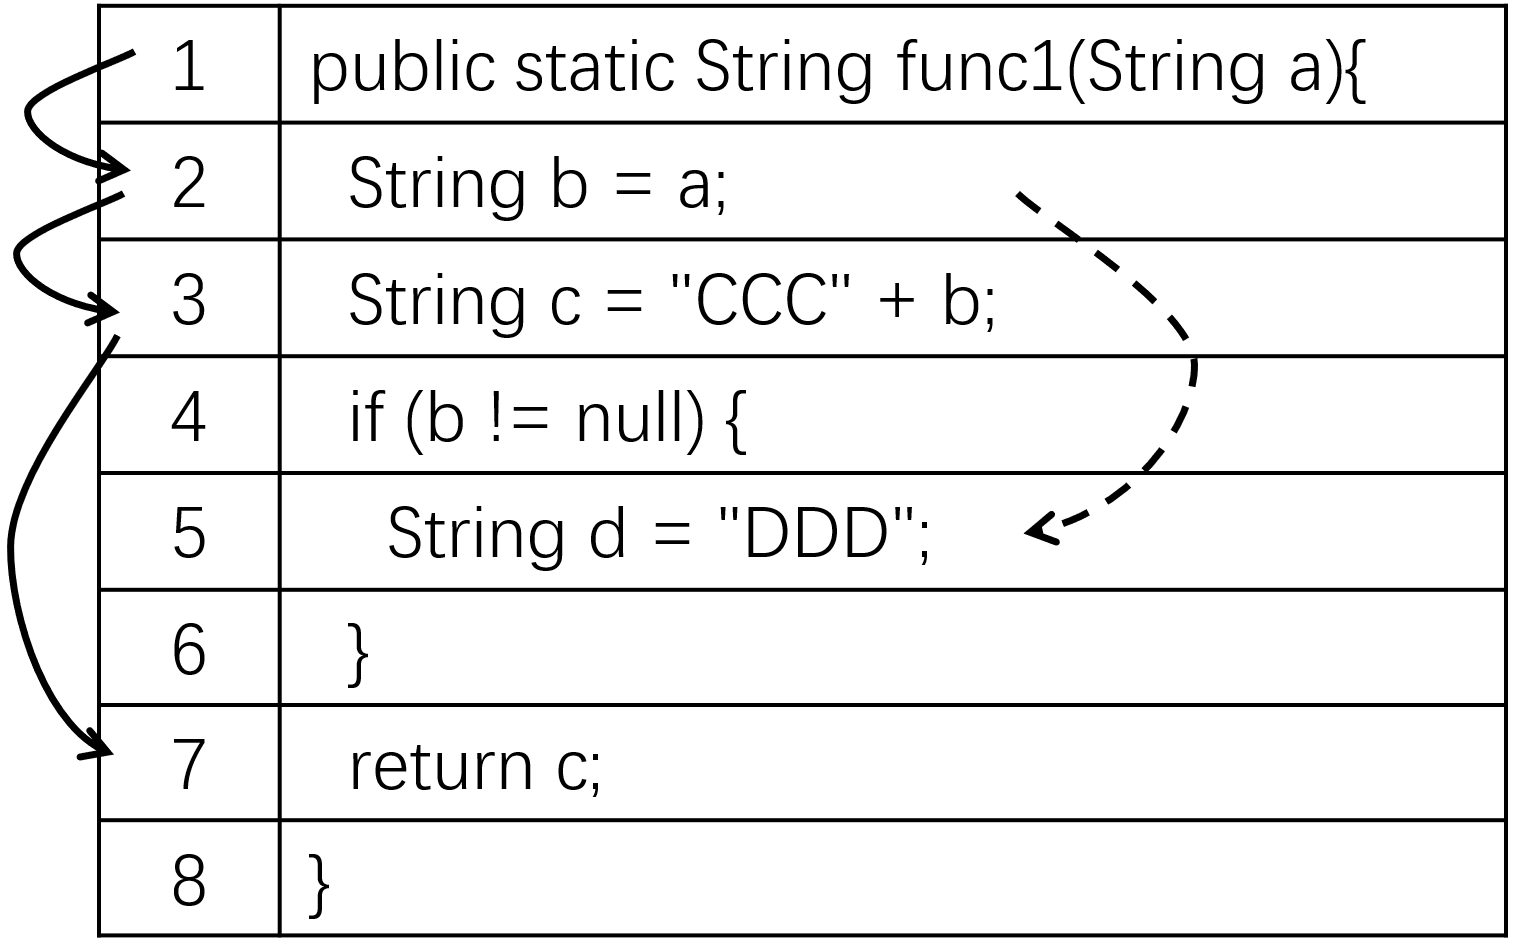
\includegraphics[width=0.5\linewidth]{FIGs/chapter2/internal_taintflow.png}
	\caption{过程内污点分析}\label{internalflow}
\end{figure}

如图~\ref{internalflow}所示,首先假设变量$a$为污点变量,实线箭头表示了显示污点传播路径,而虚线箭头表示了隐式污点传播路径,同时该图也说明了过程内污点传播基本思想,即从上至下遍历数据流图,若未标记的变量依赖于污点变量,则新变量也被标记为污点变量。虽然攻击者确实可以利用控制依赖操作数据进行攻击,但由于其分析复杂且会产生大量误报,在工程领域常常只做数据流依赖的显示分析,因此本文主要讨论显式流分析。

现代程序存在着复杂的函数调用,除了进行过程内分析,还需要进行过程间分析。其分析首先构造函数调用图(Call Graph),接着搜索存在产生点的函数,对于每一个存在产生点的函数,自顶向下分析(也可以自底向上分析)。遇到函数调用时,跟进被调函数,进行过程内污点分析,将分析结果表达为$\left\langle f, S, r\right\rangle$的函数摘要,其中$f$包含函数本身摘要信息(类名方法名和函数签名),$S$指调用过该函数后被污染的变量集合,$r$取值0或1,标记函数返回值是否被污染;接着根据函数摘要,再进行过程内分析,如此往复直至分析完函数所有代码块或是污点传播至汇聚点,报告漏洞。

\begin{figure}[!htbp]
	\centering
	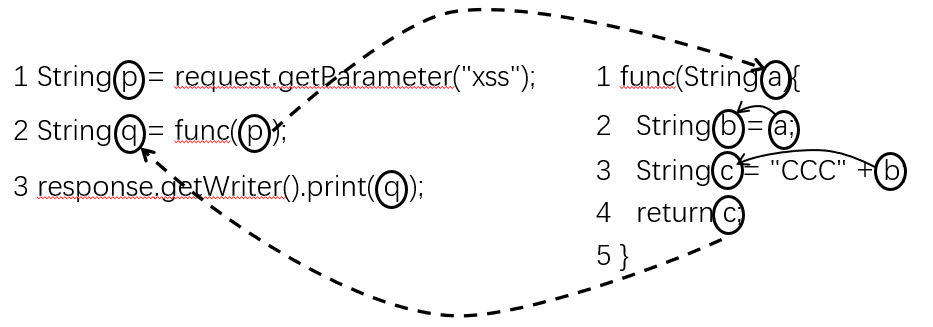
\includegraphics[width=0.7\linewidth]{FIGs/chapter2/external_taintflow.png}
	\caption{过程间污点分析}\label{externalflow}
\end{figure}

如图~\ref{externalflow}所示,分析过程从左侧函数开始,因为其找到了一处产生点——\textit{request.getParameter("xss")},于是将污点传递到变量\textit{p},接着调用函数\textit{func(p)},于是对函数\textit{func}做过程内分析,得到其函数摘要,$\left\langle func, \left\{a, b, c\right\}, 1\right\rangle$,于是回到调用者的函数内,变量\textit{q}被标记为污点,又因为第三行存在一处汇聚点——\textit{response.getpriter.print()},并且参数为污点,于是报告此处有漏洞,并且根据汇聚点可以判断该漏洞是一个 XSS 漏洞。\\

\subsection{污点分析的优势和不足}
污点分析能够对程序上下文有一定理解,往往能产生误报率相对较低以及可解释的漏洞报告,其方法对 Web 类型的安全漏洞覆盖率较高,而污点类型的漏洞普遍具有较高的危害性~\cite{taintStyle,aletheia},因此该方法已被很多工业界、学术界的安全静态扫描工具所使用~\cite{taintStyle,taint:taj,pixy},本文也选择该技术产生初步的漏洞扫描结果。

然而,污点传播仍有可能发生误报,以下通过简单示例来说明。

\begin{figure}[!htbp]
	\centering
	\subfigure[污点传播难以处理容器类型]{
		\label{taintcase1}
		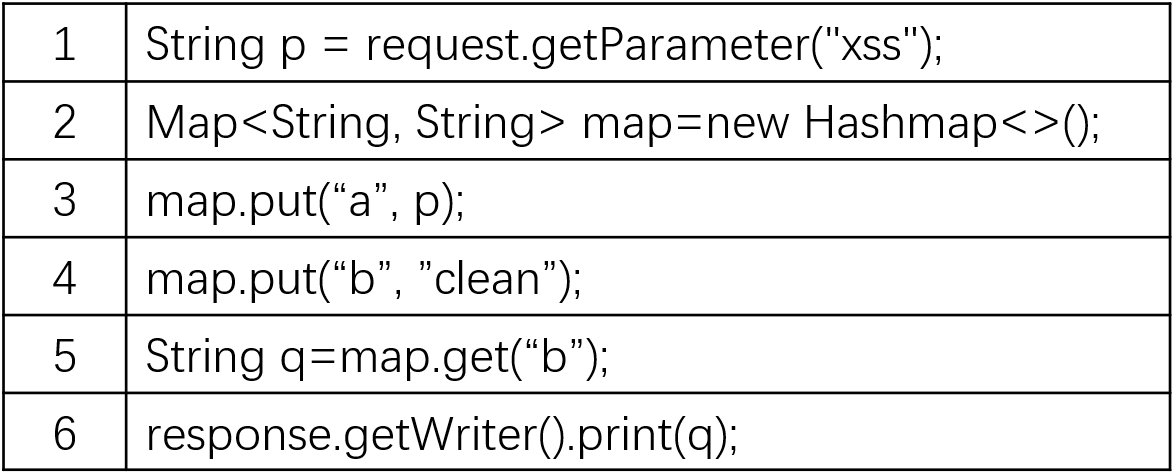
\includegraphics[width=0.4\textwidth]{FIGs/chapter2/tpcase1.png}}
	% \hspace{0.1in}
	\subfigure[污点传播难以分析控制流]{
		% \label{fig:subfig:b} %% label for second subfigure
		\label{taintcase2}
		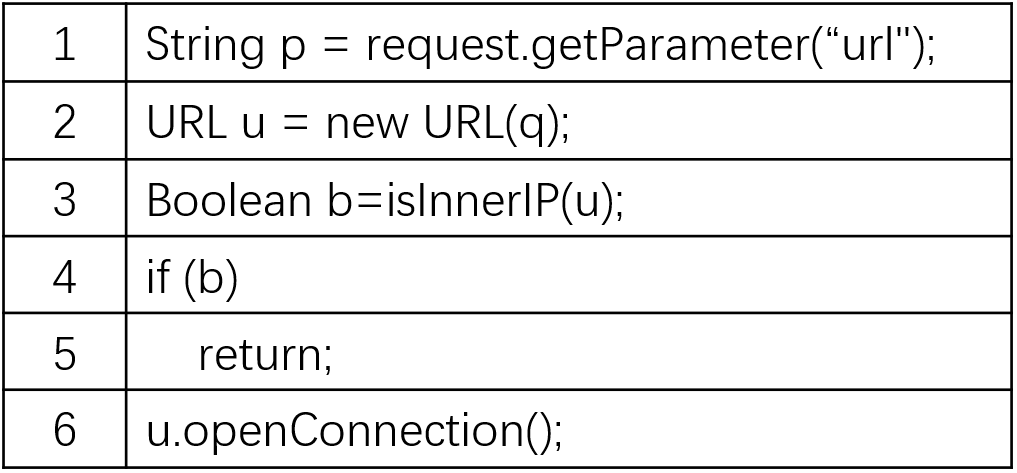
\includegraphics[width=0.4\textwidth]{FIGs/chapter2/tpcase2.png}}
	\subfigure[污点传播难以处理特殊污染条件]{
		% \label{fig:subfig:b} %% label for second subfig ure
		\label{taintcase3}
		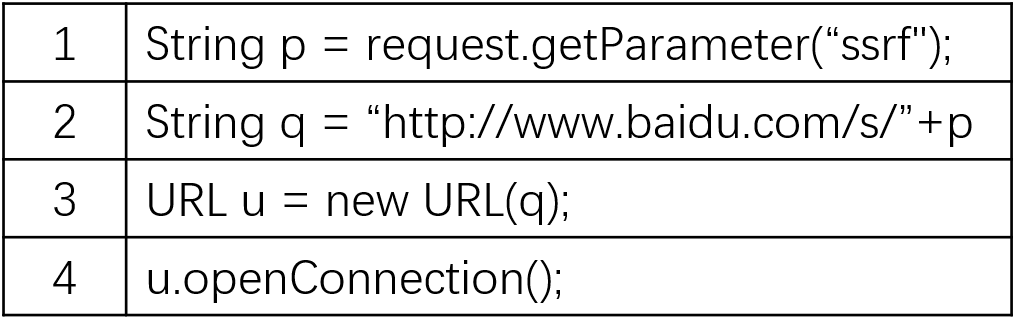
\includegraphics[width=0.4\textwidth]{FIGs/chapter2/tpcase3.png}}
	\subfigure[污点传播难以分析清洁函数]{
		% \label{fig:subfig:b} %% label for second subfigure
		\label{taintcase4}
		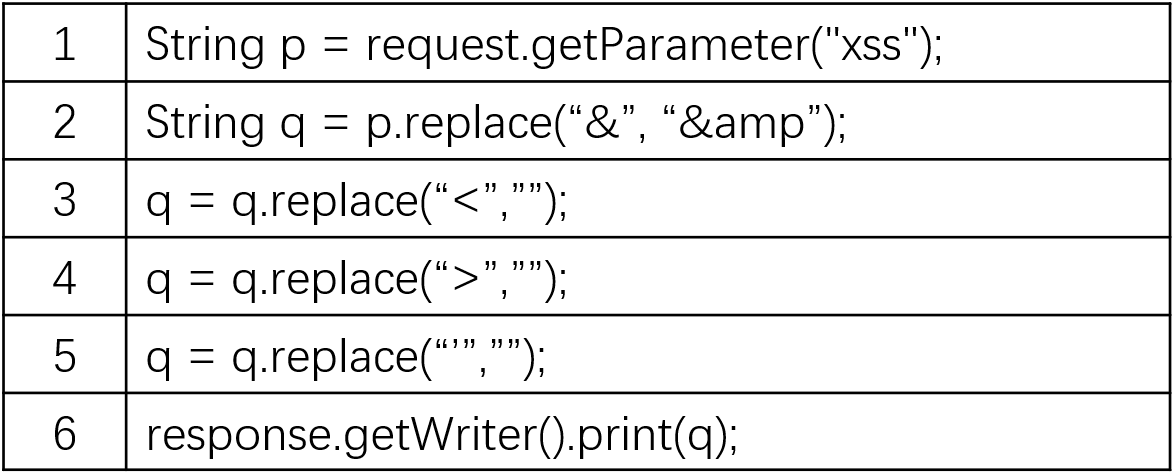
\includegraphics[width=0.4\textwidth]{FIGs/chapter2/tpcase4.png}}
	\caption{污点传播的不足}
	\label{fig:rq3} %% label for entire figure
\end{figure}
首先,污点传播对容器类型无法做很好处理,如图~\ref{taintcase1}所示,当污点传入容器类型时(在此例子中为\textit{map}),静态污点传播只能将这类变量的传播规则设为传播/不传播污点,从而造成过污染/欠污染,就如图所示,若设为\textit{map}传播污点,由于案例实际从容器中取出的是没有污点的变量,即过污染,而若设为不传播,若\textit{q}取出了参数\textit{p},那么又导致了欠污染。动态污点传播虽然解决了这一问题,但是由于其使用条件复杂,且无法用于静态分析,本文暂不讨论。

此外,静态污点传播对控制流没法做很好的处理,如图~\ref{taintcase2}所示,在第三行,程序已经对可能产生的 SSRF 漏洞进行了处理,即如果是内部地址的话则直接返回,但是不论是考虑显式流还是隐式流,污点传播都不能避免这一类误报。

再者,对于特殊触发条件的漏洞,污点传播无法很好处理,如图~\ref{taintcase3}所示,在第二行,因为 SSRF 要求攻击者能够操控主机名,所以即使用户输入的污点变量拼接在了一个正常网站之后,程序也不会出现 SSRF 的问题,而按照污点传播分析法,毫无疑问它会报告这段程序存在SSRF漏洞。

最后,不论是动态污点传播还是静态污点传播,其对污点清洁点的识别能力几乎为零,如图~\ref{taintcase4}所示,程序已经对潜在的XSS攻击做出的处理——即在第2$\sim$5行对用户输入的特殊符号进行替换和过滤,但是污点传播并不能识别这些清洁点,导致误报。    

正是因为存在这些不足,本文将在下文引入程序切片技术和 BLSTM 来降低误报率。\\

\subsection{Java污点分析工具选型}
Java上的污点分析工具有很多,如 Find Security Bugs,TAJ~\cite{taint:taj}。但对于安全扫描工具来说,除了污点传播引擎,针对漏洞定义好大量的入口点和汇聚点是扫描低漏报的重要保证。Find Security Bugs 作为较为经典的扫描工具,前人已经为预先定义了大量的污点传播入口点和汇聚点,并且支持自定义新的入口点和汇聚点,非常适合二次开发。

本系统保证准确性的手段在于利用机器学习对污点传播的误报进行改进,而不是定义大量污点传播规则,因此本文使用 Find Security Bugs 进行污点传播分析。此外,本系统解决了原版 Find Security Bugs 不能展示传播路径的问题,使其更加易用。\\

\section{程序切片技术}
\subsection{程序切片定义}
% https://www.cnblogs.com/maifengqiang/archive/2013/05/21/3090739.html
% https://hacpai.com/article/1555083057303
% 前向切片与后向切片之间关系的研究.pdf
程序切片技术是一种通过对程序分析,抽取程序中与关注点相关的一组语句集合的技术,目前广泛运用于程序调试,程序测试,优化,安全分析等领域。

该技术首次由Mark Weiser在其博士论文中提出~\cite{slices:weiser1979},他将程序切片做了如下定义:

将程序抽象为图$G\langle N,E\rangle$,$N$为程序中的语句集合,$E$为$\left\langle n,m \right\rangle$的集合,其中$n$为数据流的上一条语句,m为数据流的下一条语句。

\begin{definition}[程序状态序列(state trajectory)]
    
    若程序$P$中有长度为$k$的程序状态序列$T$,则:
    $$T=\left\langle \left\langle n_{1},s_{1} \right\rangle, \left\langle n_{2},s_{2} \right\rangle , \cdots , \left\langle n_{k},s_{k} \right\rangle \right\rangle$$
    其中$n_{i} \in N$,$s_i$为一个单射函数,记录所有变量到具体值的映射。
\end{definition}

\begin{definition}[切片准则(Slicing citerion)]
    
    若对于程序$P$有切片准则$C$,则$C=\left\langle i, V \right\rangle$,其中$i$指关注点,通常是指一条程序语句,$V$表示程序$P$中的变量子集(通常为$i$上的变量集合)。
    
\end{definition}

该切片准则决定了一个投影函数$Proj_C$:
$$
\operatorname{Proj}_{\langle i, V\rangle}(T)=\langle\operatorname{Proj}_{(i, V)}^{\prime}\left(t_{1}\right) , \cdots, \operatorname{Proj}_{\langle i, V\rangle}^{\prime}\left(t_{n}\right) \rangle
$$
其中:
$$
\operatorname{Proj}_{\langle i, V\rangle}^{\prime}(\left\langle n, s \right\rangle)=\begin{cases}
{\lambda} & {\text { if } n \neq i} \\
{\langle n, s | V \rangle} & {\text { if } n=i}
\end{cases}
$$


其中$\lambda$指空字符串,$s|V$指$V$中变量的单射函数。上式的含义是指,切片准则让我们只考虑$V$中变量的状态序列,并且只有当语句是关注点时,函数才返回状态序列,否则返回空字符。

\begin{definition}[程序切片]
    
    切片$S$为一组源程序语句的子集,它由不停地删除零条或多条原程序语句得到,同时保证$\operatorname{Proj}_{C}(T)=\operatorname{Proj}_{C^{\prime}}\left(T^{\prime}\right)$其中$T'$指切片中的状态序列,而$C'=\langle succ(i), V \rangle$,$succ(i)$指最靠近关注点$i$的语句(如果V不是$i$上的变量集合)或者就是$i$本身(如果$ V $是$i$上的变量集合)。
    
\end{definition}

按照定义,可以知道Mark Weiser实际上定义的是后向切片(backward slices),即切出对关注点造成影响的所有语句和谓词集合。对其改进后也出现了前向切片(forward slices),即切出被关注点影响的其他语句和谓词集合。\\

\subsection{程序切片技术}
%https://www.cnblogs.com/maifengqiang/archive/2013/05/21/3090739.html
程序切片技术自诞生以来,也经历了多个阶段~\cite{slices:xu2005brief},起初为Mark Weiser的概念阶段,主要通过控制流来进行程序切片;随后发展为基于依赖图的切片阶段,Ottenstein等人~\cite{slices:ottenstein1984program}首先提出了运用程序依赖图(PDG,Program Dependence Graph)进行切片,主要思想是首先对程序建立程序依赖图,再通过对程序依赖图的可达性计算进行后向切片,程序依赖图是一种反应语句数据依赖和控制依赖的一种程序中间表达形式,图中的点为单条程序语句,而图中的边则表示语句之间存在数据依赖关系,例如图~\ref{internalflow}的代码中,第三行与第二行就存在数据依赖关系,第七行与第四行则存在控制依赖关系。PDG只适用于单个函数的切片,horwitz等人~\cite{slices:horwitz1990}提出了系统依赖图(SDG, System Dependence Graph)的概念,在 PDG 的基础上,额外增加了两种边,一种边表示调用函数和被调用的直接依赖关系,另一种边描述由于边的依赖而引发的间接依赖关系,同时,前向切片也在此阶段产生;第三阶段为面向对象程序切片阶段,研究者提出将接受对象作为一个隐藏参数,结合多态解析手段,将面向对象切片问题转换为一般切片问题,使程序切片可以运用于面向对象语言。

目前已有很多工具可以对java程序进行切片,例如WALA(T.J. Watson Libraries for Analysis)~\footnote{\url{http://wala.sourceforge.net/wiki/index.php/Main_Page}}和Joana~\footnote{\url{https://pp.ipd.kit.edu/projects/joana/}}。WALA原本由IBM T.J. Watson 研究中心作为DOMO项目的一部分进行开发,在2006年,IBM将改软件转赠给社区。其主要功能包括Java类型系统和类层次分析,过程间数据流分析、指针分析和调用图构造以及上下文相关的切片等。Joana是由卡尔斯鲁厄理工学院推出,基于WALA 的一些分析手段构造的另一款 Java 切片工具,其包含指针分析,异常分析和PDG构图等复杂功能,并且其切片结果中能够更清晰的看到函数调用时实参的值,而对于污点传播类型中的自定义过滤函数,实参的值是一个很重要的特征(见图~\ref{fig:sliceresult}),因此本文选择Joana作为程序的切片器。\\
\begin{figure}[!htbp]
	\centering
	\subfigure[目标程序]{
		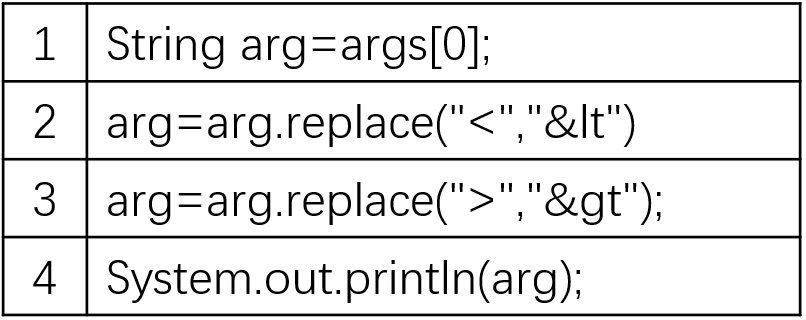
\includegraphics[width=0.42\textwidth]{FIGs/chapter2/slicetarget.png}}
	% \hspace{0.1in}
	\subfigure[Joana程序切片结果]{
		% \label{fig:subfig:b} %% label for second subfigure
		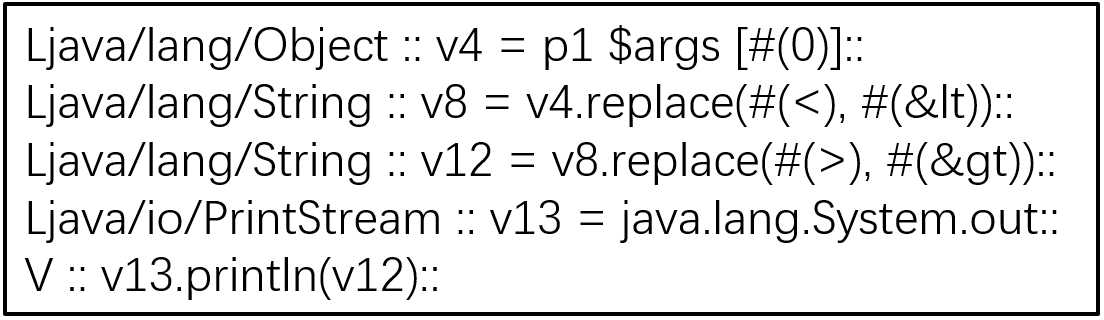
\includegraphics[width=0.42\textwidth]{FIGs/chapter2/joanaslice.png}}
	\subfigure[WALA程序切片结果]{
		% \label{fig:subfig:b} %% label for second subfigure
		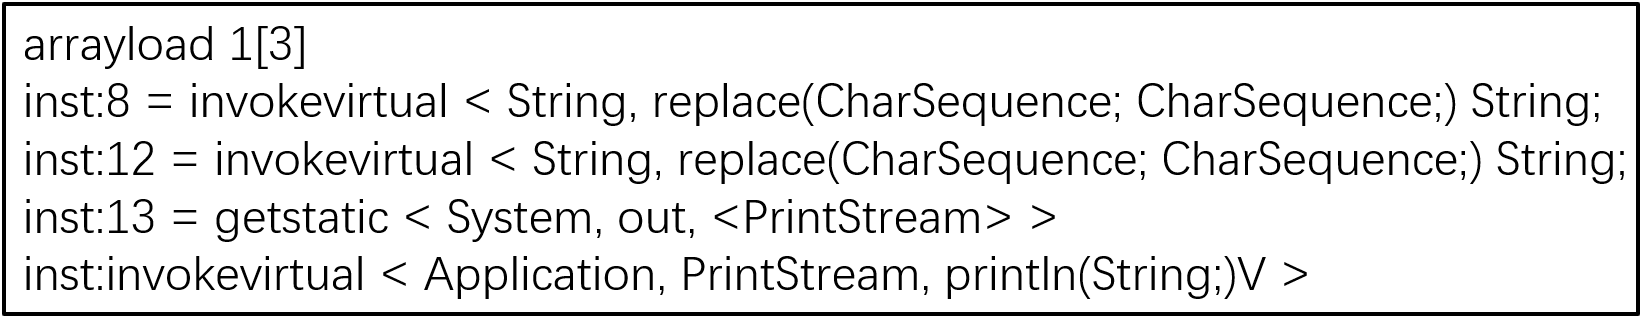
\includegraphics[width=0.85\textwidth]{FIGs/chapter2/walaslice.png}}
	\caption{Joana和WALA程序切片示例}
	\label{fig:sliceresult} %% label for entire figure
\end{figure}

\subsection{后向程序切片的优势与不足}
程序切片能够得到影响关注点的程序语句,在有效缩短了程序上下文、降低被分析代码量的同时,还能有效保留控制流的信息,在程序调试,软件度量或是软件安全中已经得到了很广泛的应用。

由于污点传播已经对程序由上而下的进行了分析,通过对汇聚点和污点值进行后向程序切片,可以从反方向分析漏洞代码,暴露先前没有考虑的控制语句,同时通过进一步的特征处理,可以作为神经网络的输入,弥补污点传播对控制流分析不足的缺陷,因此本文采用该技术作为特征处理的基础工作,另外由于程序切片属于较为传统的技术,在java语言上已有较为成熟的工具,考虑到 Java 漏洞的特征与函数参数强相关这一特性,本文选择 Joana 进行程序切片。

然而,传统后向程序切片也存在不足,目前最大的挑战在于当程序规模变大时,后向程序切片效率低下;此外原生 Joana 并不支持在缺失程序依赖下对其程序进行切片,而在 SCA 的输入中,缺失依赖的程序又是非常常见的,针对以上问题本文做出了分段切片、限制调用图切片和无依赖切片的技术调整,具体细节将在第三四章节详细说明。\\

\section{BLSTM算法}
双向长短期记忆网络(BLSTM,Bidirectional Long Short-Term Memory)是一种特殊的循环神经网络(RNN,Recurrent neural network),主要改进有双向读取和增加记忆门两方面,是一种在自然语言处理上应用广泛的神经网络~\cite{lstm:translate}。\\

\subsection{LSTM原理介绍}
为了保证在不同的序列数据上,相同数据点有不同输出结果,人们将其记忆体加入神经网络之中,从而产生了RNN,然而RNN在处理较长文本时,存在着梯度爆炸或梯度消失的问题~\cite{lstm:gradient},Hochreiter和Schmidhuber于1997年在记忆体中加入写入、输出和遗忘门,而改进后的神经网络也被成为长短期记忆网络(LSTM,Long Short-Term Memory)~\cite{lstm:1997}。

\begin{figure}[htb]
	\centering
	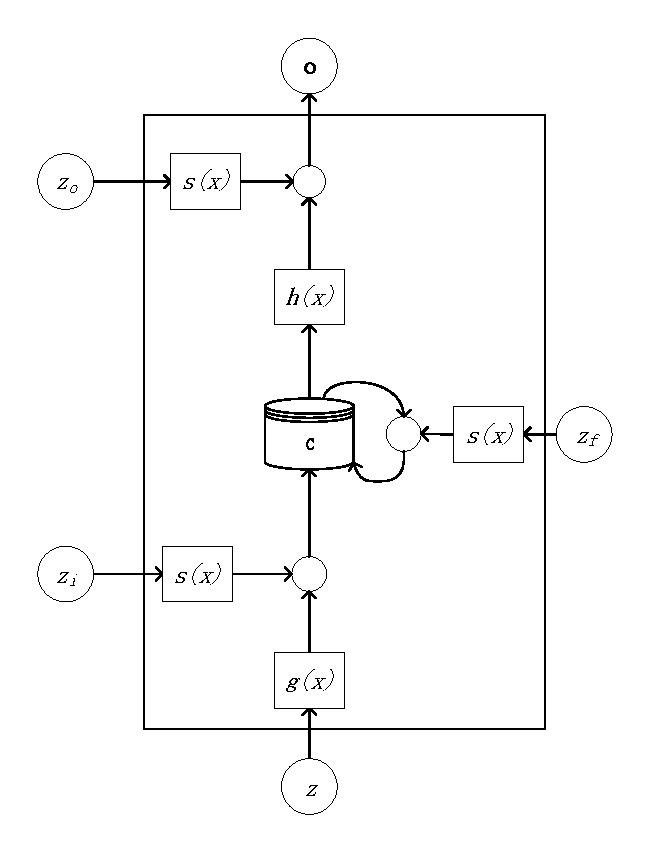
\includegraphics[width=0.4\linewidth]{FIGs/chapter2/lstm_cell.pdf}
	\caption{LSTM的神经元}\label{lstmcell}
\end{figure}
如图~\ref{lstmcell}所示,一个LSTM的神经元有四个输入:$z$表示原输入,$z_i$表示输入门,$z_f$表示遗忘门,$z_o$表示输出门,以及有一个输出$o$,神经元内有一记忆体$C$,在下一时刻的输入进入神经元时,记忆体下一时刻的值$C'=g(z)*s(z_i)+C*f(z_f)$,$g(z)$为输入值的激活函数,$s(z)$为门限的激活函数,通常取sigmoid函数,从公式可以看出,首先输入门控制了输入数据本身是否可以输入进神经元,接着遗忘门控制了记忆体中旧数据是否会保留,最后输出$a=tanh(c')*f(z_o)$,显然,$z_o$控制了记忆体是否向外输出。

\begin{figure}[htb]
	\centering
	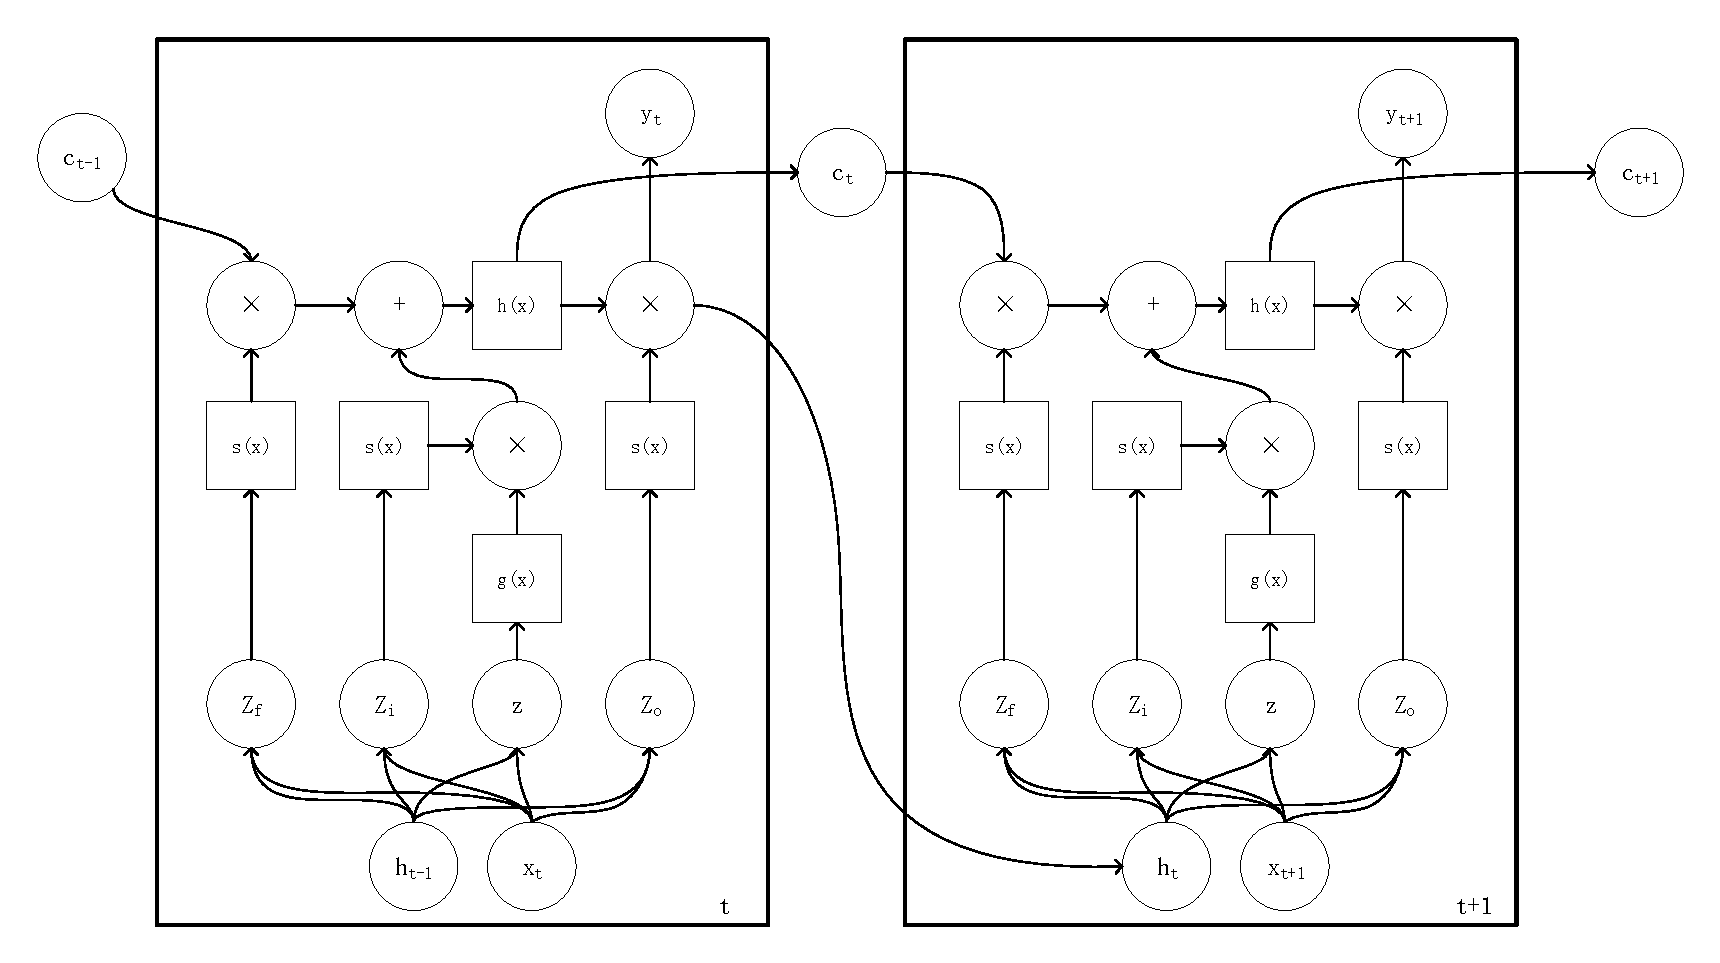
\includegraphics[width=0.8\linewidth]{FIGs/chapter2/lstm_time.pdf}
	\caption{LSTM的处理时序数据示意图}\label{lstmtime}
\end{figure}

利用LSTM处理时序数据情况如图~\ref{lstmtime}所示,对于任意时刻$t$,有$h_{t-1}$和$c_{t-1}$($t_0$时为随机值),$h_{t-1}$和$x_t$通过线性变换得到$z_f$、$z_i$、$z$和$z_o$,例如,$z_f=W_{f}\times [h,x]+b_{f}$。$z_f$、$z_i$、$z$和$z_o$均为以为向量,其长度等于该层LSTM神经元的个数,按上文所述,这4组向量输入神经元,结合神经元内的记忆体$c_{t-1}$计算得到输出$y_t$,同时$y_t$的值也作为下一轮输入的一部分,即$h_t$。$h_t$和$x_t+1$作为下一时刻的输入,输入下一时刻的神经元。在自然语言处理领域,人们通常利用最后一个时刻的输出对自然语言分类。\\

\subsection{双向读取——BLSTM}
早在RNN时期,就有研究者提出双向RNN提升拟合或预测准确性的思想,而LSTM作为RNN的一种,自然也可以运用该思想对其进行优化。

\begin{figure}[htb]
	\centering
	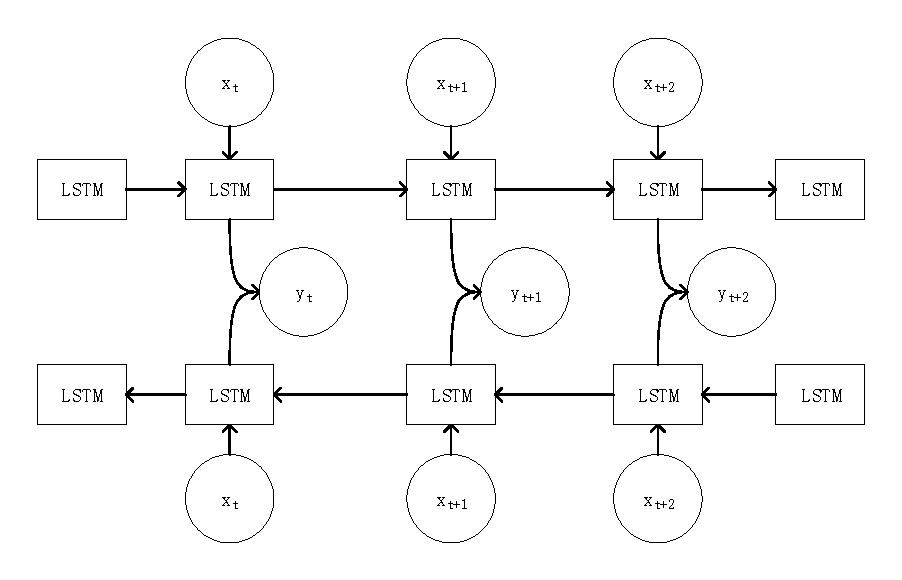
\includegraphics[width=0.8\linewidth]{FIGs/chapter2/blstm.pdf}
	\caption{BLSTM处理时序数据示意图}\label{blstm}
\end{figure}
如图~\ref{blstm}所示,对于一组时序数据$X=\left\{ x_0,\dots,x_t,x_{t+1},\dots,x_{k} \right\}$,训练两个LSTM网络,第一个网络正向读取数据(如图上方所示),第二个网络逆向读取数据(如图下方所示),在同一时刻,结合两个方向的网络输出值作为该时刻的输出(如果用于分类问题,通常结合正向$t_k$的输出和逆向$t_0$的输出)。


\subsection{BLSTM 的优势}

BLSTM的优势在于,单向LSTM在$x_t$时刻的输出实际上只被$x_0, x_1, \dots, x_t$影响,即其只能考虑截止到当前时刻的数据,而BLSTM的在某一时刻的输出值不仅受到该时刻正向数据的影响,还能受到该时刻后向数据的影响,因此有纵观全局的能力。\\

LSTM 增加了门限机制,解决了RNN 梯度爆炸或梯度消失的问题,而 BLSTM 通过双向传播机制,能够综合正向时序和逆向时序信息,是时序数据的分类和拟合问题(如自然语言处理问题)较为合适的算法。而目前已有很多利用自然语言处理和该模型进行程序分析的研究~\cite{naturalSoftware,lstm:recognize,lstm:repo,vuldeepecker,Koc2017,Koc2019}。所以本系统采用 BLSTM 作为污点传播预测算法,将污点传播的切片作为上下文敏感的自然语言数据,通过训练集训练 BLSTM 参数将其保存,在给定污点传播的切片输入时,系统调用训练好的模型对其进行预测。

\section{Django 框架}
\subsection{Django 框架简介}
Django 是一个高级的 Python Web 开发框架~\footnote{\url{https://www.djangoproject.com/}},它使开发者能够对 Web 应用进行简洁实用的设计并对其进行快速开发。Django 由一群有经验的开发者开发,其框架和内部设计避免了很多 Web 开发的问题,帮助开发者只关心于他们Web应用本身的逻辑而不需要重新开发通用组件。

Django 采用模型视图模板(MVT,Model-View-Template)模式,在模型层,其有一套高效的对象关系映射(ORM,Object Relational Mapping)框架和一些常用对象,比如用户对象,管理员对象等;在视图层,Django 阶级了基于正则表达式的URL分派系统,能够让用户灵活的处理自己的 URL 路由,并且内置的 Request,Response 对象能够让开发者快速的获取和返回数据;在模板层,Django 有自己的原生模板引擎,类似于 Jinja2,同时支持用户更换第三方引擎,保证用户充分自由的展现其数据。除此之外,Django 还内置了一个用户管理后台和各类安全保障模块,使大大加速了开发者的开发过程。\\

\subsection{Django 框架优势}
本系统的后台主要是对机器学习模型的操作,因此自然选择了 Python 开发语言,而 Django 作为 Python 语言上应用最为广泛的Web开发框架之一,自然也成为了本系统后台的首选技术。
利用 Django 的灵活性,本系统利用其 URL 分派系统接受客户端传来的预测、训练、标记等请求并对其处理,通过 ORM 框架将程序切片、模型训练数据快速本地化,以完成对系统后台的快速开发。

\section{本章小结}
本章首先介绍了目前流行的漏洞挖掘技术,并对其优劣势进行了说明,接着介绍了本系统使用的技术、工具和框架,并分别说明了使用这些技术、工具和框架的原因。在技术角度,本章依次介绍了污点分析技术、程序切片技术和 BLSTM 神经网络并对其优缺点进行了总结,分析了使用后向程序切片和 BLSTM 对污点传播会使污点分析更精确的原因;在工具角度,本章指出了使用 Find Security Bugs 进行污点分析,使用 Joana 进行程序切片的原因及本系统对其进行的优化改进;最后简单介绍了Django框架以及其优点。

\chapter{Java静态安全扫描工具需求分析与设计}
\section{系统整体概述}
Java语言通常用于Web服务和Android程序开发,其中的大量安全漏洞类型可以通过污点传播分析法进行扫描,然而随着漏洞种类和开发方式不断丰富,污点分析存在失误,因此产生了大量误报,为此安全工程师不得不修改污点传播规则,以增加漏报为代价换取低误报,或是人工对大量误报漏洞判断,这两种做法无疑会增加潜在安全风险。

本系统旨在提供对于Java代码的更精确的漏洞静态扫描功能,在源代码开发阶段进行代码安全扫描。相对于传统污点传播扫描工具,本系统结合了程序切片和BLSTM,从已有的误报漏洞片段进行分析,降低污点传播误报率。系统总体架构如图~\ref{overview}所示,系统主要分为前端和后端两大部分,前端部分运行在用户端,包含污点分析模块、程序切片模块、部分预测模块,而在扫描系统后端运行在服务器端,包含预处理模块,另一部分预测模块和数据库。

污点分析模块对开源的find-sec-bugs做改进,使之能够输出污点传播树,为误报预测提供基础数据;程序切片模块分析污点传播树,将其拆分为子污点传播流,利用Joana生成SDG并进行切片;数据预处理模块将切片模块的输出数据进行泛化和向量化处理,使之可以输出预测模块;误报预测模块利用切片模块的子污点传播流和其对应切片,通过BLSTM进行切片预测,从而对漏洞进行预测。本系统采用客户端采用Java进行开发,管理后台和程序预测服务由Python和Django开发。

\begin{figure}[htb]
	\centering
	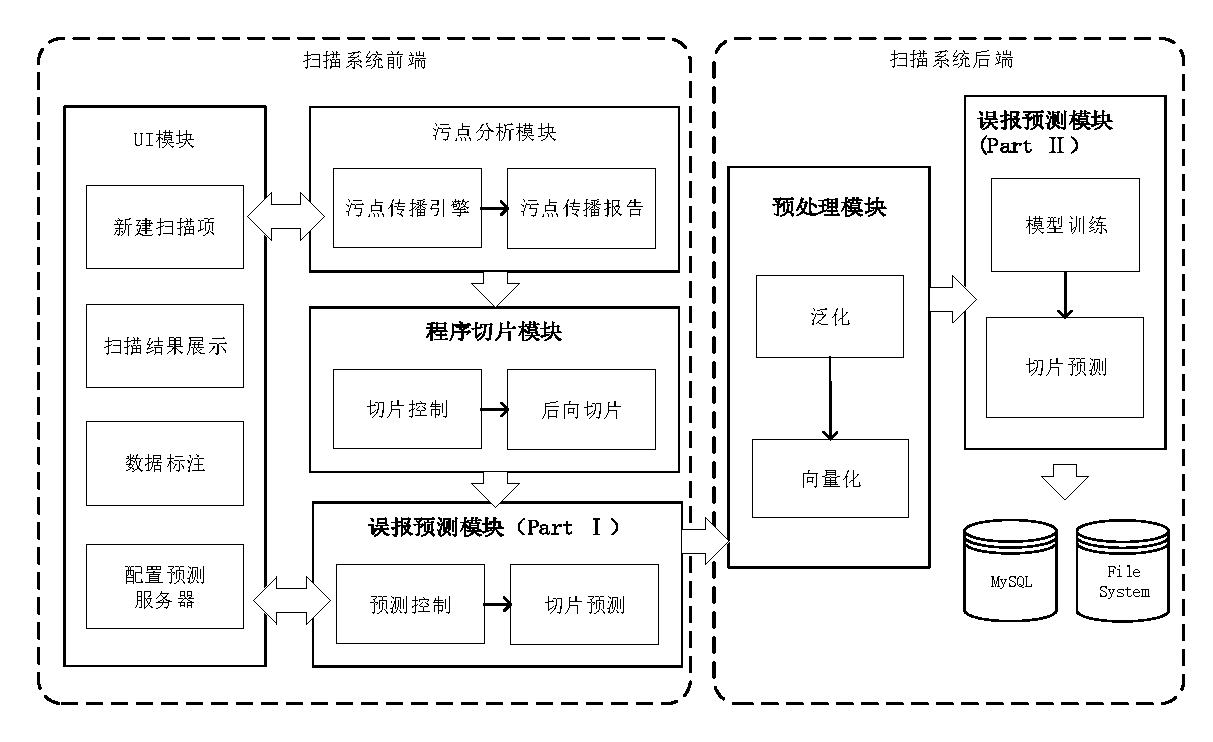
\includegraphics[width=5in]{FIGs/chapter3/system-architecture.pdf}
	\caption{系统总体架构图}\label{overview}
\end{figure}

\section{系统需求分析}
\subsection{功能性需求}
本系统功能性需求分析按污点分析模块,程序切片模块,预处理模块和误报预测模块四个方面进行。

污点分析模块由污点分析引擎对用户提交的jar文件进行扫描,产生初步结果,该模块所涉及的功能性需求如表~\ref{dmd:taint}所示,其主要功能为污点分析,而对于用户来说,系统需要友好的展现污点分析结果,即存在构造污点传播树和查看分析结果的需求,污点传播树由污点传播图构造而来,因此存在构造污点传播图需求,此外,污点分析是一项耗时操作,用户(尤其是开发工程师)可能会对一次污点分析结果进行保存,交给安全工程师进行漏洞验证,因此系统最好还需有保存分析结果和读取分析结果功能。
\begin{table}[!htbp]\footnotesize %label table
	\centering
	\caption{污点分析模块功能性需求列表}
	\vspace{2mm}
	% l - left, r - right, c - center. | means one vertical line 这里声明的是表格单元中的内容如何对齐
	\begin{tabular}{L{1.3cm}L{2.5cm}L{6.8cm}L{1.5cm}}
		\toprule
		\textbf{需求编号}&\textbf{需求名称}&\textbf{需求内容}&\textbf{优先级}\\
		\midrule
		R1	& 污点分析 				& 对于用户上传的代码进行污点分析,包括了过程内分析和过程间分析 & 高 \\
		R2  & 构造污点传播图 	 & 对于代码中存在的汇聚点,构造其污点传播图 & 高 \\
		R3  & 构造污点传播树	 & 对于一个污点传播类型的分析结果,用户最终看到一棵或多课污点传播树,其由污点传播图构造,一张污点传播图可能有多棵传播树,一个传播树上清晰标注有一个产生点和一个汇聚点 & 高 \\
		R4  & 查看分析结果	 & 对于一个污点传播类型的分析结果,用户最终看到一棵或多课污点传播树,对于树上的叶子节点,用户能够知晓其代码位置 & 高 \\
		R5  & 保存分析结果	   &用户可以对当前代码的漏洞分析详情进行保存,其中关键点在于对污点传播树进行序列化 & 中 \\
		R6  & 读取分析结果 	   &用户可以对保存后的分析结果文件进行读取,二次查看漏洞详情,其中关键点在于对污点传播树结构的反序列化 & 中 \\
		\bottomrule
	\end{tabular}
	\label{dmd:taint}
\end{table}

程序切片模块对污点分析结果进行切片处理,该模块所涉及的功能性需求如表~\ref{dmd:slice}所示,该模块的主要功能是根据污点分析模块的分析结果进行后向程序切片,将其拆解,得到四个子需求,首先其需要污点分析的结果进行处理,接着对污点传播树进行拆分,对于每一个污点传播流,其包含有若干个子污染流,下一步对这些需求进行后向切片,最后将切片结果转换为有一定结构的文本。

\begin{table}[!htbp]\footnotesize %label table
	\centering
	\caption{程序切片模块功能性需求列表}
	\vspace{2mm}
	% l - left, r - right, c - center. | means one vertical line 这里声明的是表格单元中的内容如何对齐
	\begin{tabular}{L{1.3cm}L{2.5cm}L{6.8cm}L{1.5cm}}
		\toprule
		\textbf{需求编号}&\textbf{需求名称}&\textbf{需求内容}&\textbf{优先级}\\
		\midrule
		R7	 & 处理污点分析结果 & 对污点分析的结果进行处理,对于每一个漏洞实例,反序列化的污点传播树并转化为适用于切片的传播树表达形式 & 高 \\
		R8	 & 污点传播树拆分 & 将每一个传播树拆分为多个子污点传播流,每一个污点传播流包含若干个<函数入口点,关注点>对(其为一个切片的单位) & 高 \\
		R9   & 后向程序切片 & 对于每一个<函数入口点,关注点>, 结合用户上传的Jar包,进行后向程序切片 & 高 \\
		R10 & 输出切片结果	 & 对于切片,程序能将其表示为文本,即对切片结构体序列化 & 高 \\
		\bottomrule
	\end{tabular}
	\label{dmd:slice}
\end{table}

预处理模块对切片结果进行预处理,该模块所涉及的功能性需求如表~\ref{dmd:preprocessing}所示,该模块的主要功能是对切片文本进行泛化和向量化,在泛化需求主要保证一个切片能代表一类代码片段;随后进行向量化,对于切片的单词序列进行token标记,从而产生字典和切片向量,即BLSTM模型的输入。此外,一个较低优先级的需求为根据字典,将切片向量还原为切片的单词序列。

\begin{table}[!htbp]\footnotesize %label table
	\centering
	\caption{预处理模块功能性需求列表}
	\vspace{2mm}
	% l - left, r - right, c - center. | means one vertical line 这里声明的是表格单元中的内容如何对齐
	\begin{tabular}{L{1.3cm}L{2.5cm}L{6.8cm}L{1.5cm}}
		\toprule
		\textbf{需求编号}&\textbf{需求名称}&\textbf{需求内容}&\textbf{优先级}\\
		\midrule
		R11   & 泛化 & 对于每一个切片进行泛化处理,包括抽象数值、字符串、类名和方法名等 & 高 \\
		R12 & 向量化	 & 对于一个切片的单词序列,生成单词与整形值的字典并按字典对其向量化 & 高 \\
		R13 & 反向量化	 & 对于一个单词序列的向量,根据字典将其还原为切片的单词序列 & 低 \\
		\bottomrule
	\end{tabular}
	\label{dmd:preprocessing}
\end{table}

误报预测模块是对保障漏洞报告准确性的核心模块,包括客户端、后端和Web前端部分,该模块所涉及的功能性需求如表~\ref{dmd:predict}所示,该模块的需求主要为对给定漏洞实例进行预测,标记以及模型训练。预测依赖后端服务,因此有设置后端服务器的需求;预测分为预测切片安全性需求和预测漏洞真实性需求,分别由后端服务和客户端实现;标记分为对切片安全性标记和漏洞真实性标记,当漏洞标记为误报时,用户需指定安全的污染流;同时,管理员有训练预测模型的需求;此外,由于预测过程并不是很占用资源,对保存预测结果的需求程度较低;最后用户可以清空标记和预测结果。

\begin{table}[!htbp]\footnotesize %label table
	\centering
	\caption{误报预测模块功能性需求列表}
	\vspace{2mm}
	% l - left, r - right, c - center. | means one vertical line 这里声明的是表格单元中的内容如何对齐
	\begin{tabular}{L{1.3cm}L{2.5cm}L{6.8cm}L{1.5cm}}
		\toprule
		\textbf{需求编号}&\textbf{需求名称}&\textbf{需求内容}&\textbf{优先级}\\
		\midrule
		R14 & 预测切片安全性 & 对于一个切片向量,预测该切片是否是安全的(污染流无法传播) & 高 \\
		R15 & 标记切片安全性	 & 对切片向量,标记其是否安全 & 高 \\
		R16 & 预测漏洞真实性 & 用户在客户端可以查看预测结果,即该漏洞是否真实存在,需要结合切片预测需求 & 高 \\
		R17 & 标记漏洞真实性	 & 用户在客户端可以对于一个漏洞,标记漏洞是否存在,不存在时用户需提供理由(指出安全的污染流) & 高 \\
		R18 & 训练预测模型	 & 管理员可以在Web页面发起训练模型任务,或是安排定时器定期更新模型 & 高 \\
		R19 & 保存预测结果	 & 用户在客户端可以保存漏洞预测结果 & 低 \\
		R20 & 清空标记和预测结果	 & 用户在客户端可以清空标记和预测结果,以便重新预测 & 低 \\
		R21 & 设置预测服务器	 & 用户在客户端设置远程服务器 & 中 \\
		\bottomrule
	\end{tabular}
	\label{dmd:predict}
\end{table}


\subsection{非功能性需求}
本系统旨在为开发者和安全工程师提供Java代码安全扫描功能,考虑到系统功能性质、使用场景和所属领域,系统的非功能性需求主要有高效率,健壮性,保密性,安全性和扩展性五点。

首先,本系统的功能点在于对Java代码进行安全扫描,其使用场景位于软件开发至测试阶段,因此扫描过程要保证一定的效率和健壮性,如果一次扫描等待时间过长,或是扫描过程中途崩溃,那么开发过程就会受到影响,甚至影响整个服务的可用性,因此本系统需要是高效且健壮的。

其次,本系统涉及软件安全领域,很可能是恶意攻击者的首要攻击对象,因此自身需要具备保密性和安全性,这里的保密性是指保证用户提交的Java代码和Jar包的数据安全,安全性是指扫描服务本身经过充分安全性测试,不出现安全漏洞。

最后,很多企业目前已经拥有了适用于自身特点的基于污点传播的扫描器,为此,系统需要保证一定的扩展性,如将污点传播的解析抽象为接口,保证其可以基于任意污点传播工具进行预测。\\

\subsection{系统用例描述}\label{sec:case}
%用例图
本系统的主要用户为软件开发工程师和软件安全运营人员,根据对系统需求的分析,得到系统用例如图~\ref{fig:case}所示, 软件开发工程师和运营人员均有基于污点分析的静态扫描、扫描结果切片和预测、漏洞实例标记这三个用例,其中基于污点分析的静态扫描存在两例扩展用例,即保存污点分析结果和读取分析结果,漏洞实例标记实际包含了标记正报结果和标记误报结果用例,安全运营人员还多出模型训练和发放客户端口令的用例。

\begin{figure}[!htbp]
	\centering
	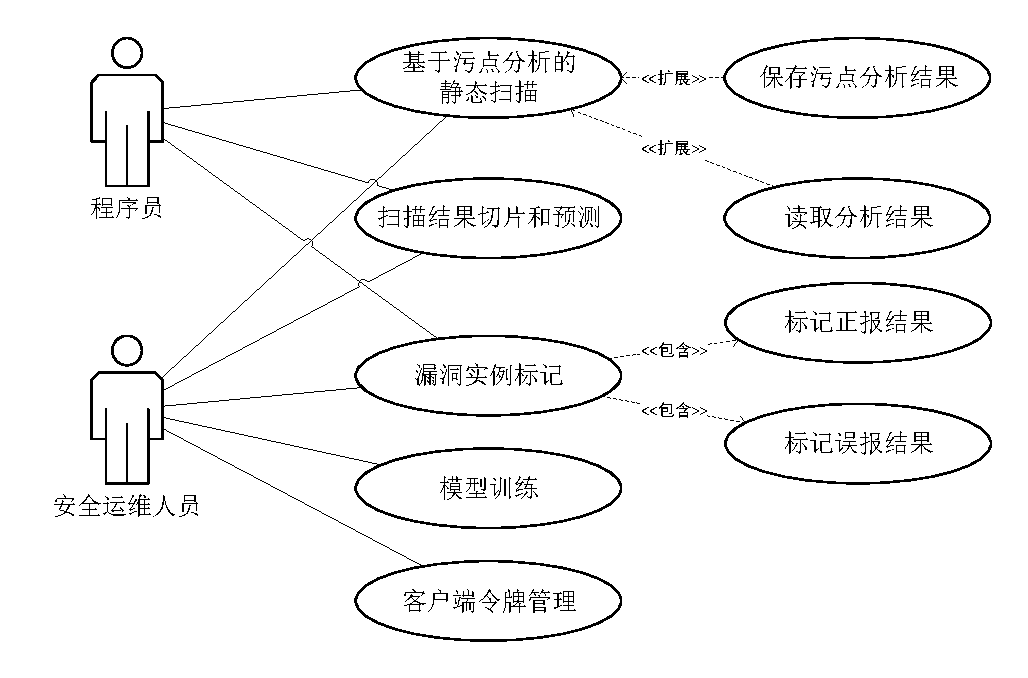
\includegraphics[width=5in]{FIGs/chapter3/case.pdf}
	\caption{系统用例图}\label{fig:case}
\end{figure}

\newcounter{caseCounter}
\setcounter{caseCounter}{1}

基于污点分析进行程序的静态扫描是本系统的基本功能,同样也是漏洞预测的基础。其用例描述如表~\ref{case:taint}所示,安全工程师或软件工程师(下面统称“用户”)对将开发好的项目进行构建,新建项目时将源代码和构建得到的Jar/War包添加到项目中,随后系统对其进行污点分析,并返回给用户潜在的安全漏洞。
% 1基于污点分析的静态扫描
\begin{table}[!htb]\footnotesize %label table
	\centering
	\caption{基于污点分析的静态扫描用例描述}
	\vspace{2mm}
	% l - left, r - right, c - center. | means one vertical line 这里声明的是表格单元中的内容如何对齐
	\begin{tabular}{L{3cm}L{10cm}}
		\toprule
		\textbf{描述项}&\textbf{说明}\\
		\midrule
		用例编号 & C\arabic{caseCounter}\stepcounter{caseCounter} \\
		用例名称 & 基于污点分析的静态扫描用例 \\
		对应功能需求编号  & R1, R2, R3, R4 \\ 
		参与者 & 用户 \\
		前置条件 & 用户已开发好项目并已构建的Jar/War包 \\
		后置条件 & 无\\
		正常流程 & \tabincell{l}{
							1. 用户选择“文件”,“新建项目”,打开新建项目会话框\\
							2. 用户输入项目名称,选择需要分析的包文件以及源文件所在目录\\
							3. 用户点击“分析”按钮,程序开始对其进行基于污点分析的静态扫描\\
							4. 用户在界面上看到漏洞列表,点击一个污点传播类型的漏洞\\
							5. 用户在界面上看到该漏洞的污点传播树\\
							6. 用户点击任意污点传播树的叶子节点,在界面上看到对应的源代码
					}\\
		异常流程 & 2. 若出现异常,则弹出异常会话框并显示异常信息\\
		\bottomrule
	\end{tabular}
	\label{case:taint}
\end{table}

% 2保存分析结果
污点分析后,用户可以对其分析结果进行保存,其用例描述见表~\ref{case:taintsave},用户点击保存按钮后,系统将污点传播树的每一节点序列化漏洞注解,并将含有一组注解的一系列漏洞保存为本地文件。

\begin{table}[!htb]\footnotesize %label table
	\centering
	\caption{保存污点分析结果用例描述}
	\vspace{2mm}
	% l - left, r - right, c - center. | means one vertical line 这里声明的是表格单元中的内容如何对齐
	\begin{tabular}{L{3cm}L{10cm}}
		\toprule
		\textbf{描述项}&\textbf{说明}\\
		\midrule
		用例编号 & C\arabic{caseCounter}\stepcounter{caseCounter}  \\
		用例名称 & 保存污点分析结果用例 \\
		对应功能需求编号  & R5 \\ 
		参与者 & 用户  \\
		前置条件 & 用户已创建项目且进行了基于污点分析的静态扫描 \\
		后置条件 & 用户指定位置出现保存好的分析报告\\
		正常流程 & \tabincell{l}{
			1. 用户选择“文件”,“另存为”,打开另存为对话框\\
			2. 用户输入保存文件名、文件类型和保存位置,点击保存按钮,分析结果\\被保存
		}\\
		异常流程 & 2. 若出现异常,则弹出异常会话框并显示异常信息\\
		\bottomrule
	\end{tabular}
	\label{case:taintsave}
\end{table}

% 3读取分析结果
对于以保存的分析结果,用户可以加载它们重新分析漏洞结果,程序对分析结果反序列化后在界面显示先前分析结果,如表~\ref{case:taintload}所示。

\begin{table}[!htb]\footnotesize %label table
	\centering
	\caption{读取分析结果用例描述}
	\vspace{2mm}
	% l - left, r - right, c - center. | means one vertical line 这里声明的是表格单元中的内容如何对齐
	\begin{tabular}{L{3cm}L{10cm}}
		\toprule
		\textbf{描述项}&\textbf{说明}\\
		\midrule
		用例编号 & C\arabic{caseCounter}\stepcounter{caseCounter}  \\
		用例名称 & 读取分析结果用例 \\
		对应功能需求编号  & R6 \\ 
		参与者 & 用户  \\
		前置条件 & 用户磁盘中已有一份污点分析报告 \\
		后置条件 & 无\\
		正常流程 & \tabincell{l}{
			1. 用户选择“文件”,“打开”,显示打开文件对话框\\
			2. 用户在打开文件对话框中选择报告文件,点击“打开”按钮,程序\\加载并在界面上显示污点分析报告中的内容
		}\\
		异常流程 & 2. 若出现异常,则弹出异常会话框并显示异常信息息\\
		\bottomrule
	\end{tabular}
	\label{case:taintload}
\end{table}

% 4设置预测服务器
对于客户端来说,对漏洞进行标记或者预测前提需要设置远程服务器,设置预测服务器的用例描述如表~\ref{case:setserver}所示,用户通过管理员发放的token和服务器地址设置远端服务器。
\begin{table}[!htb]\footnotesize %label table
	\centering
	\caption{设置预测服务器用例描述}
	\vspace{2mm}
	% l - left, r - right, c - center. | means one vertical line 这里声明的是表格单元中的内容如何对齐
	\begin{tabular}{L{3cm}L{10cm}}
		\toprule
		\textbf{描述项}&\textbf{说明}\\
		\midrule
		用例编号 & C\arabic{caseCounter}\stepcounter{caseCounter}  \\
		用例名称 & 设置预测服务器用例 \\
		对应功能需求编号  & R21 \\ 
		参与者 & 用户  \\
		前置条件 & 管理员已向用户发放token \\
		后置条件 & 无\\
		正常流程 & \tabincell{l}{
			1. 用户选择“AI”,“Set Server”,显示服务器设置对话框\\
			2. 用户服务器对话框汇中设置服务器地址以及token信息\\
			3. 用户点击“验证”按钮,检查配置是否正确\\
			4. 用户点击“应用”按钮,完成服务器配置
		}\\
		异常流程 & 2. 若出现异常,则弹出异常会话框并显示异常信息\\
		\bottomrule
	\end{tabular}
	\label{case:setserver}
\end{table}

% 5扫描结果预测
扫描结果切片和预测功能是本系统的最核心功能,程序首先对污点传播结果分析,拆解为污点传播片段并分别切片,再由服务端预测每一个切片是否为清洁片段,最后得出漏洞实例是否为真实漏洞。涉及的用例描述如表~\ref{case:predict}所示。

\begin{table}[!htbp]\footnotesize %label table
	\centering
	\caption{扫描结果切片和预测用例描述}
	\vspace{2mm}
	% l - left, r - right, c - center. | means one vertical line 这里声明的是表格单元中的内容如何对齐
	\begin{tabular}{L{3cm}L{10cm}}
		\toprule
		\textbf{描述项}&\textbf{说明}\\
		\midrule
		用例编号 & C\arabic{caseCounter}\stepcounter{caseCounter}  \\
		用例名称 & 扫描结果切片和预测用例 \\
		对应功能需求编号  & R7, R8, R9, R10, R14, R16 \\ 
		参与者 & 用户  \\
		前置条件 & 用户已完成远程服务器配置并且已有污点分析结果 \\
		后置条件 & 预测所需所有切片信息发送至服务器\\
		正常流程 & \tabincell{l}{
			1. 用户选择“AI”点击“Slice and Predict”,程序开始对污点分析结\\果进行切片和预测\\
			2. 用户等待切片和预测完成时,可以在弹出的会话框中观察预测进度,\\并随时取消预测\\
			3. 用户在程序主界面看到每一漏洞预测结果,预测为误报的漏洞由灰色\\图标标识且在漏洞列表标注为“(P: FP)”,预测结果为正报的漏洞图标\\不变,文字标注为“(P: TP)”\\
			4. 用户在点击一个漏洞,在污点传播图上可以看到预测解释,当预测结果\\为误报时,所有与预测为安全的污点传播流相关的叶子节点由“(*)”标\\注。
		}\\
		异常流程 & 2. 若出现异常,则弹出异常会话框并显示异常信息\\
		\bottomrule
	\end{tabular}
	\label{case:predict}
\end{table}

% 6标记正报结果
若漏洞实例被安全工程师判断为真实存在的,工程师可以对该漏洞标记为正报,此时所有污染流片段均自动标记为不安全,并且发送给服务端。标记正报结果用例描述如表~\ref{case:labeltp}所示。

\begin{table}[!htbp]\footnotesize %label table
	\centering
	\caption{标记正报结果用例描述}
	\vspace{2mm}
	% l - left, r - right, c - center. | means one vertical line 这里声明的是表格单元中的内容如何对齐
	\begin{tabular}{L{3cm}L{10cm}}
		\toprule
		\textbf{描述项}&\textbf{说明}\\
		\midrule
		用例编号 & C\arabic{caseCounter}\stepcounter{caseCounter}  \\
		用例名称 & 标记正报结果用例 \\
		对应功能需求编号  & R15, R17 \\ 
		参与者 & 用户  \\
		前置条件 & 用户已经对污点分析结果进行了切片和预测 \\
		后置条件 & 用户指定漏洞的所有污染流片段均标记为不安全且发送至服务器\\
		正常流程 & \tabincell{l}{
			1. 用户右键点击需要标记的正报漏洞实例,弹出标记菜单\\
			2. 用户点击“Labeled as True Positive”,该漏洞被标记为正报,漏洞说\\明内容被显示为“[L: TP]”
		}\\
		异常流程 & 2. 若出现异常,则弹出异常会话框并显示异常信息\\
		\bottomrule
	\end{tabular}
	\label{case:labeltp}
\end{table}

% 7标记误报结果
若漏洞实例被用户判断为不存在,用户可以对该漏洞标记为误报,此时用户需要指定一条最短的污染流,并且在该污染流中污点消失,同时,这段“安全的污染流”被发送至服务端。标记误报结果用例描述如表~\ref{case:labelfp}所示。

\begin{table}[!htb]\footnotesize %label table
	\centering
	\caption{标记误报结果用例描述}
	\vspace{2mm}
	% l - left, r - right, c - center. | means one vertical line 这里声明的是表格单元中的内容如何对齐
	\begin{tabular}{L{3cm}L{10cm}}
		\toprule
		\textbf{描述项}&\textbf{说明}\\
		\midrule
		用例编号 & C\arabic{caseCounter}\stepcounter{caseCounter}  \\
		用例名称 & 标记误报结果用例 \\
		对应功能需求编号  &  R15, R17 \\ 
		参与者 & 用户  \\
		前置条件 & 用户已经对污点分析结果进行了切片、预测或标记 \\
		后置条件 & 无\\
		正常流程 & \tabincell{l}{
			1. 用户右键点击需要标记的误报漏洞实例,弹出标记菜单\\
			2. 用户点击“Labeled Safe Flow”,弹出误报标记会话框\\
			3. 用户选择一条最短的安全污染流,同时看到该污染流的哈希和切片信\\息,点击确定后完成标记\\
			4. 用户看到其所标记的漏洞被标注为“[L: FP]”,并且在污染传播树中,\\所有与被用户标记的那段污染流相关的叶子节点由“[*]”标记。
		}\\
		异常流程 & 2. 若出现异常,则弹出异常会话框并显示异常信息\\
		\bottomrule
	\end{tabular}
	\label{case:labelfp}
\end{table}

% 8清空切片、标记和预测结果
由于切片、预测是复杂操作,系统会将其放入缓存,同时标记结果用户也会有想清空的情况,因此本系统提供一键清除切片、标记和预测结果的功能。其用例描述如表~\ref{case:clean}所示。
\begin{table}[!htb]\footnotesize %label table
	\centering
	\caption{清空切片、标记和预测结果用例描述}
	\vspace{2mm}
	% l - left, r - right, c - center. | means one vertical line 这里声明的是表格单元中的内容如何对齐
	\begin{tabular}{L{3cm}L{10cm}}
		\toprule
		\textbf{描述项}&\textbf{说明}\\
		\midrule
		用例编号 & C\arabic{caseCounter}\stepcounter{caseCounter}  \\
		用例名称 & 清空切片、标记和预测结果用例 \\
		对应功能需求编号  & R20 \\ 
		参与者 & 用户  \\
				前置条件 & 用户已经对污点分析结果进行了切片和预测 \\
		后置条件 & 用户指定漏洞的最短安全污染流被标记为安全且发送至服务器\\
		正常流程 & \tabincell{l}{
			1. 用户选择“AI”点击“Clean DB”,程序清空切片、预测和标记数据,\\并在漏洞的预测标签上显示“(P: UNK)”,在标记标签上显示“[L: UNK]”
		}\\
		异常流程 & 无\\
		\bottomrule
	\end{tabular}
	\label{case:clean}
\end{table}

% 9模型训练
模型训练的用例描述如表~\ref{case:train}所示,管理员通过在Web后端发起模型训练请求,系统会进行异步调用,通过消息队列,训练程序会根据选择的训练配置进行模型训练,并将训练模型保存,供预测时调用,用户也可以设置定时任务,是系统按时自动训练模型。
\begin{table}[!htb]\footnotesize %label table
	\centering
	\caption{模型训练用例描述}
	\vspace{2mm}
	% l - left, r - right, c - center. | means one vertical line 这里声明的是表格单元中的内容如何对齐
	\begin{tabular}{L{3cm}L{10cm}}
		\toprule
		\textbf{描述项}&\textbf{说明}\\
		\midrule
		用例编号 & C\arabic{caseCounter}\stepcounter{caseCounter}  \\
		用例名称 & 模型训练用例 \\
		对应功能需求编号  & R11, R12, R18 \\ 
		参与者 & 用户(这里特指安全运营人员)  \\
		前置条件 & 数据库中已存在用于训练的切片和标记数据 \\
		后置条件 & 数据库中记录已经训练好的模型\\
		正常流程 & \tabincell{l}{
			1. 用户登录 Web 控制台\\
			2. 用户在控制台中点击“Model Config”进入模型配置页面,查看或新\\建模型配置\\
			3. 用户在控制台中点击“Periodic Tasks”,进入任务页面,在任务页面\\
			中选择模型训练任务,并设置任务类型(定时任务或单次执行任务)并\\且指定时间,以及训练指定的模型配置,系统到规定时间后自动训练模\\型
		}\\
		异常流程 & \tabincell{l}{4. 若模型训练中遇到错误,将错误信息返回到任务结果表中,\\供用户查看}\\
		\bottomrule
	\end{tabular}
	\label{case:train}
\end{table}

客户端令牌管理的用例描述如表~\ref{case:train}所示,管理员通过在Web后端对客户端令牌进行管理,即对其进行增删改查操作。
\begin{table}[!htb]\footnotesize %label table
	\centering
	\caption{客户端令牌管理用例描述}
	\vspace{2mm}
	% l - left, r - right, c - center. | means one vertical line 这里声明的是表格单元中的内容如何对齐
	\begin{tabular}{L{3cm}L{10cm}}
		\toprule
		\textbf{描述项}&\textbf{说明}\\
		\midrule
		用例编号 & C\arabic{caseCounter}\stepcounter{caseCounter}  \\
		用例名称 & 客户端令牌管理用例 \\
		对应功能需求编号  & R21 \\ 
		参与者 & 安全运营人员  \\
		前置条件 & 无 \\
		后置条件 & 无 \\
		正常流程 & \tabincell{l}{
			1. 用户登录 Web 控制台\\
			2. 用户在控制台中点击“Client Token”进入客户端令牌管理页面,对客\\户端令牌进行增加,修改,删除等操作。
		}\\
		异常流程 & 无 \\
		\bottomrule
	\end{tabular}
	\label{case:token}
\end{table}

\section{系统总体设计}
本系统的框架图已在本节第一章图~\ref{overview}展示,下面将对系统设计的模块从逻辑视图、开发视图、进程视图、物理视图和场景视图五个方面~\cite{4+1view}详细介绍系统总体设计。% The 4+1 View Model of Architecture,Philippe Kruchten 

% 逻辑视图=UML类
本系统的逻辑视图如图~\ref{view:logic}所示,该视图主要反应了本系统的对象设计,图中 AbstractTaintDetector 是污点传播分析类的抽象类,与之相关的类有MethodDescriptor 和 Location ,其分别表示函数摘要和代码位置;
AbstractIncjectionDetector 是注入类型漏洞分析器的抽象类,继承自 AbstractTaintDetector,相对于 AbstractTaintDetector 其主要增加了具有输出漏洞报告的功能,目前几乎所有污点传播漏洞类都继承该类;
与 AbstractIncjectionDetector 相关的有 InjectionSink 类,该类表示污点汇聚点,其记录汇聚点可产生污点传播图,即 TaintFlowGraph 类;
与 TaintFlowGraph 相关的有 TaintTreeGenerator ,即污点传播树生成类,其用于生成污点传播树,树上节点为 TreeNode 类;
NodeAnnotation 是树节点注解类,用于在用户界面上显示一个污点传播树的叶子节点;
若干棵污点传播树共同构成了一个漏洞实例——BugInstance类;若干个BugInstance类组合产生BugCollection,即一个项目的漏洞集合类;
SliceRunner 为切片控制类,其首先调用报告翻译器对漏洞报告进行翻译,产生污点项目类——TaintProject,接着调用切片器对程序进行切片,最终产生切片项目类——SliceProject;Parser 和 Slicer 分别为翻译器和切片器的接口;
SpotbugsReportParser 为 Spotbugs 的报告翻译器,实现了翻译器接口,负责筛选 FindSecBugs 的污点传播类型漏洞并进行翻译;
JoanaSlicer 为基于 Joana 的切片器,实现切片器接口;
切片项目中包含切片的集合,切片类为 Slice;
PredictRunner 为预测控制类其依赖预测器接口——Predictor 对漏洞实例进行预测,返回为预测项目类——PredictProject 的实例;
BLSTMRemotePredictor 为远程调用服务端预测接口的预测器,实现 Predictor 接口;
后端服务器的所有服务表示为 Service 类,其中包含对 BLSTM 模型的控制类 ModelController;
表示预处理的类有 Preprocessing 类,该类中有对切片的各类泛化操作,以及 Tokenizer 类,其中包含对切片的向量化和反向量化操作;
最后模型类表示为 BLSTM 类;其通过数据集 Dataset 类进行训练。

\begin{figure}[!htb]
	\centering
	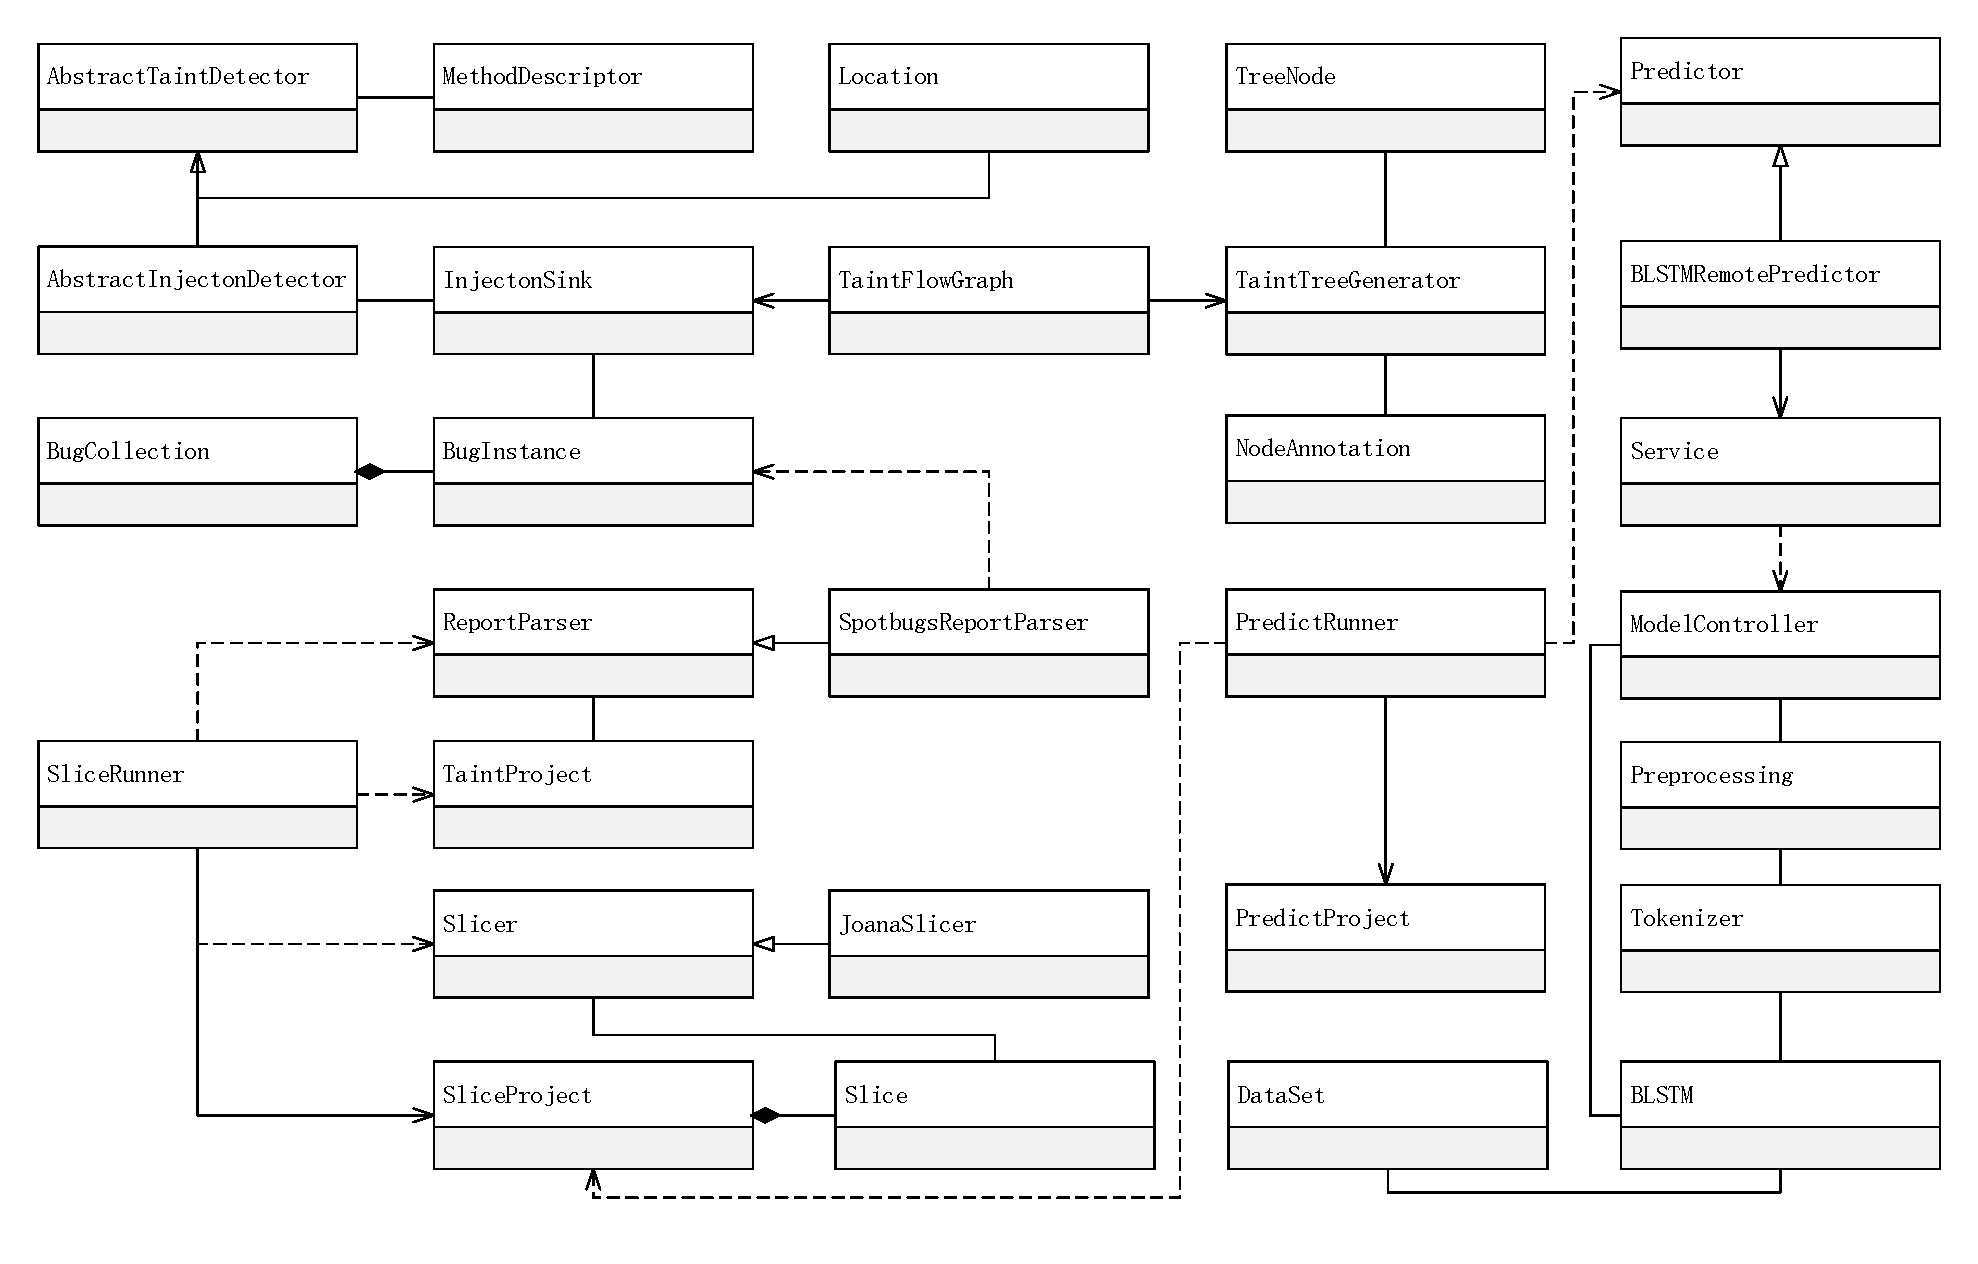
\includegraphics[width=5in]{FIGs/chapter3/viewlogic.pdf}
	\caption{系统逻辑视图}\label{view:logic}
\end{figure}

本系统的开发视图如图~\ref{view:dev}所示,该视图以开发者角度描述了模块的静态组织结构,具体来说本系统分为用户界面(UI),服务(Service)和第三方依赖包(Third-part Dependency)组成。

UI主要包括了客户端包和管理员Web端包;Service中存在污点分析(TaintAnalysis)包,切片(Slice)包,Joana切片器(Joana)包,预处理(Preprocessing)包,预测模块客户端包(PredictCli)和服务端(PredictSrv)包,以及用于表示各种数据的 Data 包;第三方依赖包中主要有 Spotbugs 和 FindSecBugs,Spotbugs 包含了基本GUI界面和数据流分析框架,FindSecBugs包括了基本污点分析引擎,Joana 为本系统选用的切片器,Pytorch 用于构建 BLSTM 模型,Django 框架用于构建后端服务,Celery 和 Redis 用于训练请求的异步调用。

\begin{figure}[!htb]
	\centering
	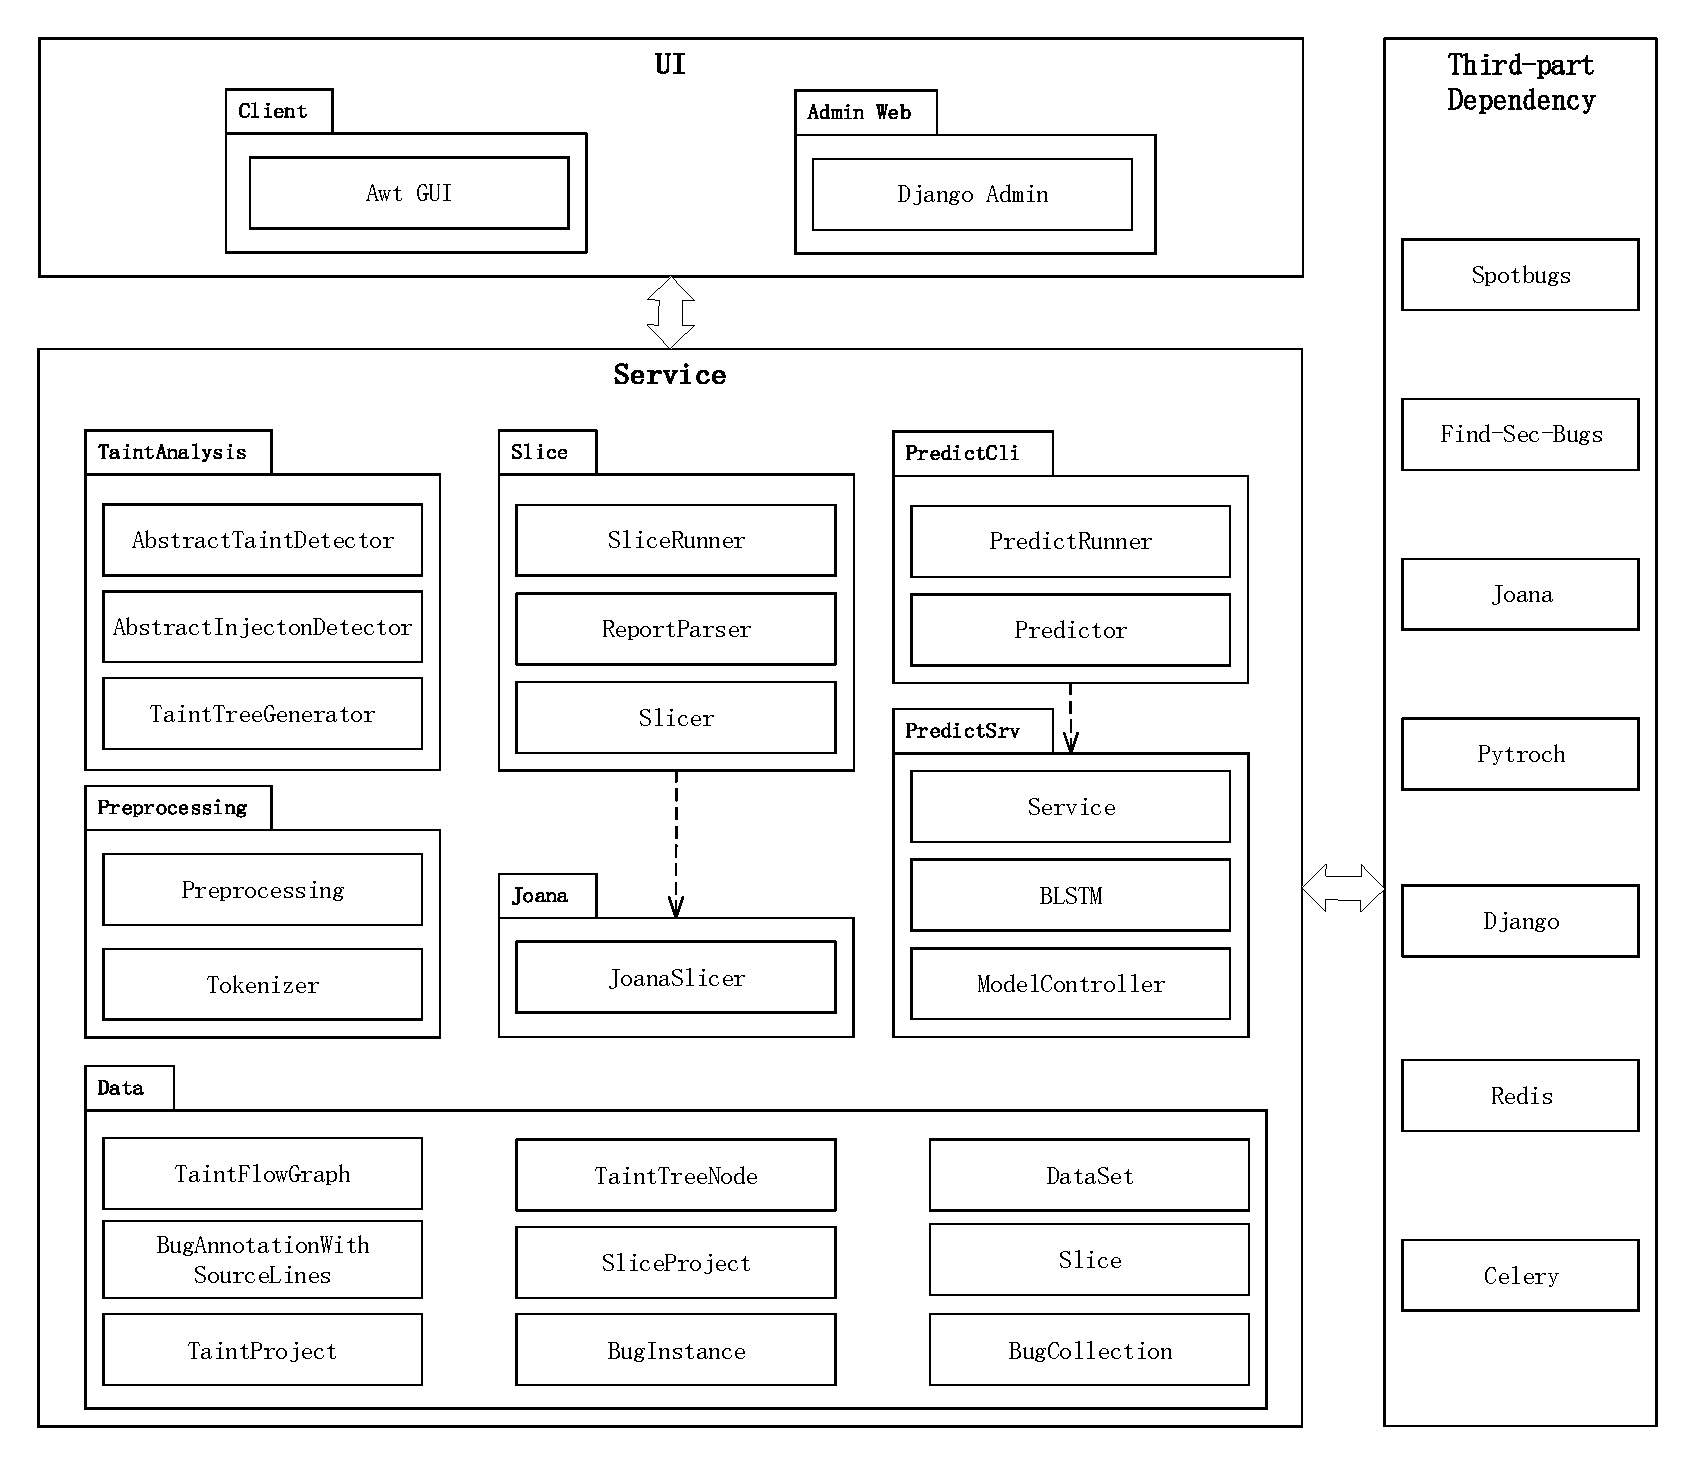
\includegraphics[width=5in]{FIGs/chapter3/viewdev.pdf}
	\caption{系统开发视图}\label{view:dev}
\end{figure}

本系统的进程视图如图~\ref{view:process}所示,用户端有管理端浏览器进程和代码扫描客户端进程,这两个进程通过 HTTP 协议与后端服务进程通信,服务进程通过TCP与模型训练任务进程和数据库进程通信,模型训练进程监听训练任务队列消息,收到训练消息后则开始模型训练,期间与数据库进程通信,获取训练配置信息。

\begin{figure}[!htb]
	\centering
	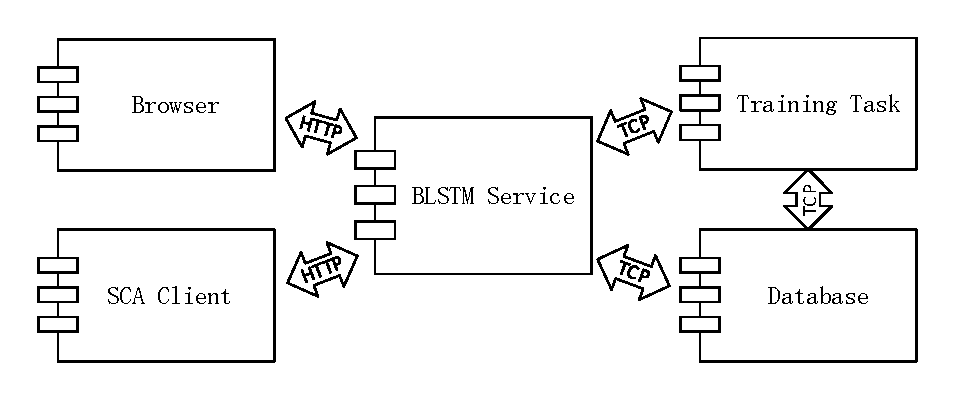
\includegraphics[width=0.7\textwidth]{FIGs/chapter3/viewprocess.pdf}
	\caption{系统进程视图}\label{view:process}
\end{figure}

本系统的物理视图如图~\ref{view:physical}所示,该视图在部署方面描述了本系统的架构。

在用户端部分,主要功能集中于扫描客户端,其包括了 GUI 界面和核心 jar 包(Core.jar),核心 Jar 包中含污点分析、切片和一部分预测模块。管理员用过浏览器使用本系统,主要完成发布模型训练任务、发放客户端 Token 或是管理数据对象的操作。

用户端通过HTTP与应用服务器通信,应用服务器上部署了基于BLSTM预测的 Web 应用,以及配置好的 Django 管理员后台应用,服务器上还部署了 Celery Work,以便使管理员可以发布关于模型训练的异步任务和定时任务,训练数据和已经训练好的模型直接存放在服务器的文件系统上。

服务端通过TCP与数据库连接,MySQL 数据库主要存放本系统的各种实体数据,Redis 数据库供 Celery 使用。
\begin{figure}[!htb]
	\centering
	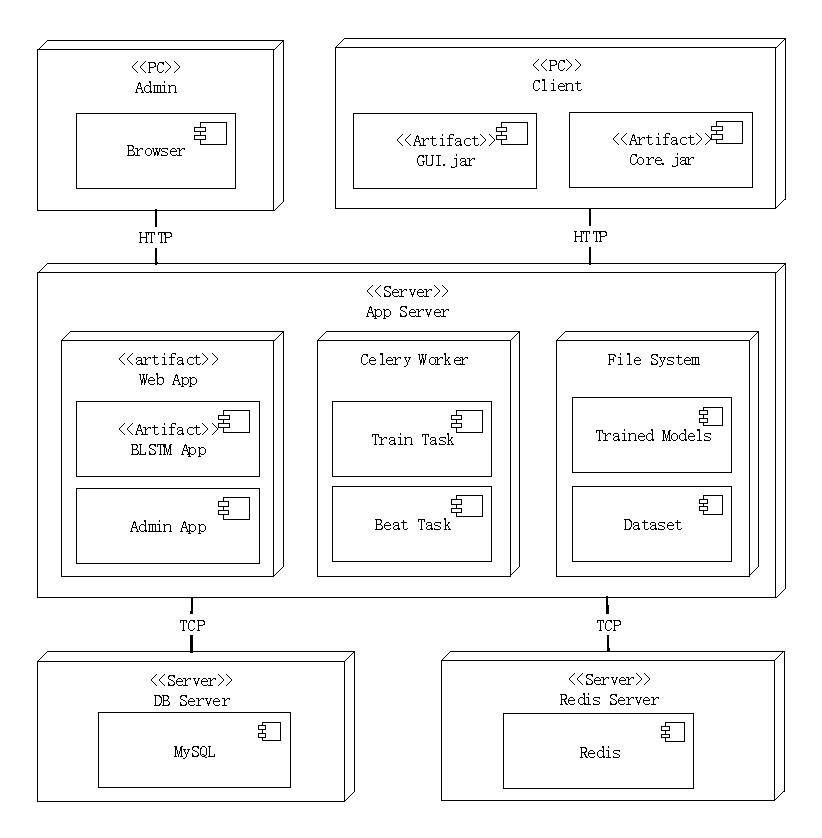
\includegraphics[width=0.7\textwidth]{FIGs/chapter3/viewphysical.pdf}
	\caption{系统物理视图}\label{view:physical}
\end{figure}

本系统的场景视图即用例图(图~\ref{fig:case}),在~\ref{sec:case} 章已经详细说明。

\section{污点分析模块设计}

污点分析模块是系统的基础模块,以用户提交的Jar包为输入,输出污点分析报告,本节分析流程和涉及到的类图两方面,说明该模块的设计。由于本模块主要是对FindSecBugs进行改进,使之可以在报告中输出污点传播树,因此本节只说明改进部分和与改进部分相关的类和流程,说明重点,对其它部分进行一部分简化。\\

\subsection{流程设计}
本系统的污点分析模块流程如图~\ref{taintprocess} 所示,首先用户输入被扫描的jar包对象,模块初始化漏洞报告,即产生一个空漏洞实例集合;接着其调用分析器对每一个类进行分析,对于第i个类,模块会对类函数的CFG进行拓扑排序,再依次对$i$类中的每个函数$k$进行污点分析,在污点分析时,本模块需要记录关于污点传播的有关信息,包括函数$k$内调用指令(如 \textit{invokestatic}、\textit{invokedynamic}、\textit{invokeinterface} 等)位置、函数返回指令位置(如 \textit{ireturn}、\textit{areturn}、\textit{dreturn} 等)和与污点汇聚点相关的代码语句位置信息,以便之后通过污点传播图和传播树产生漏洞报告。

污点传播最终报告内容为污点传播树,但是污点实际上是以图的形式进行传播的,因此本模块设计在漏洞报告阶段先生成污点传播图,再根据图生成污点传播树。

当应用中类和函数分析完后,模块会遍历所有污点汇聚点,这些污点汇聚点在分析时产生,记录了存在漏洞的汇聚点本身以及与污点传播到汇聚点的所有函数调用信息,对于每个汇聚点,利用汇聚点信息和分析时记录的函数调用语句位置,函数返回语句位置产生污点传播图。

最后,根据污点传播图构造污点传播树,并将传播树表示为能由GUI展示的漏洞实例对象,放入漏洞集合中,当所有汇聚点遍历完成后,模块最终输出漏洞实例的集合。

\begin{figure}[!htb]
	\centering
	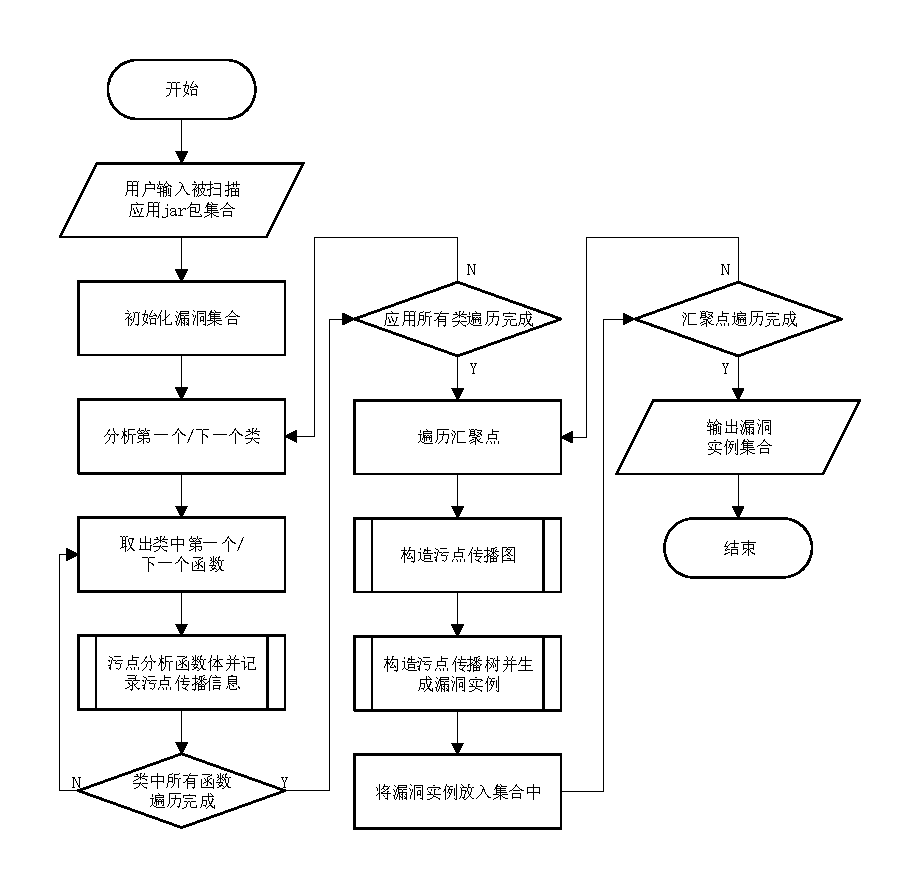
\includegraphics[width=0.8\textwidth]{FIGs/chapter3/taintprocessing.pdf}
	\caption{污点分析模块流程图}\label{taintprocess}
\end{figure}

图中记录污点传播信息、构造污点传播图和构造污点传播树的流程较为复杂,将在第~\ref{sec:taintImp} 节中详细说明。\\

\subsection{污点传播图类图设计}

为了方便图的遍历,污染传播图的数据结构采用邻接链表的形式,其类图设计如图~\ref{taintGraphClass} 所示。

\begin{figure}[!htb]
	\centering
	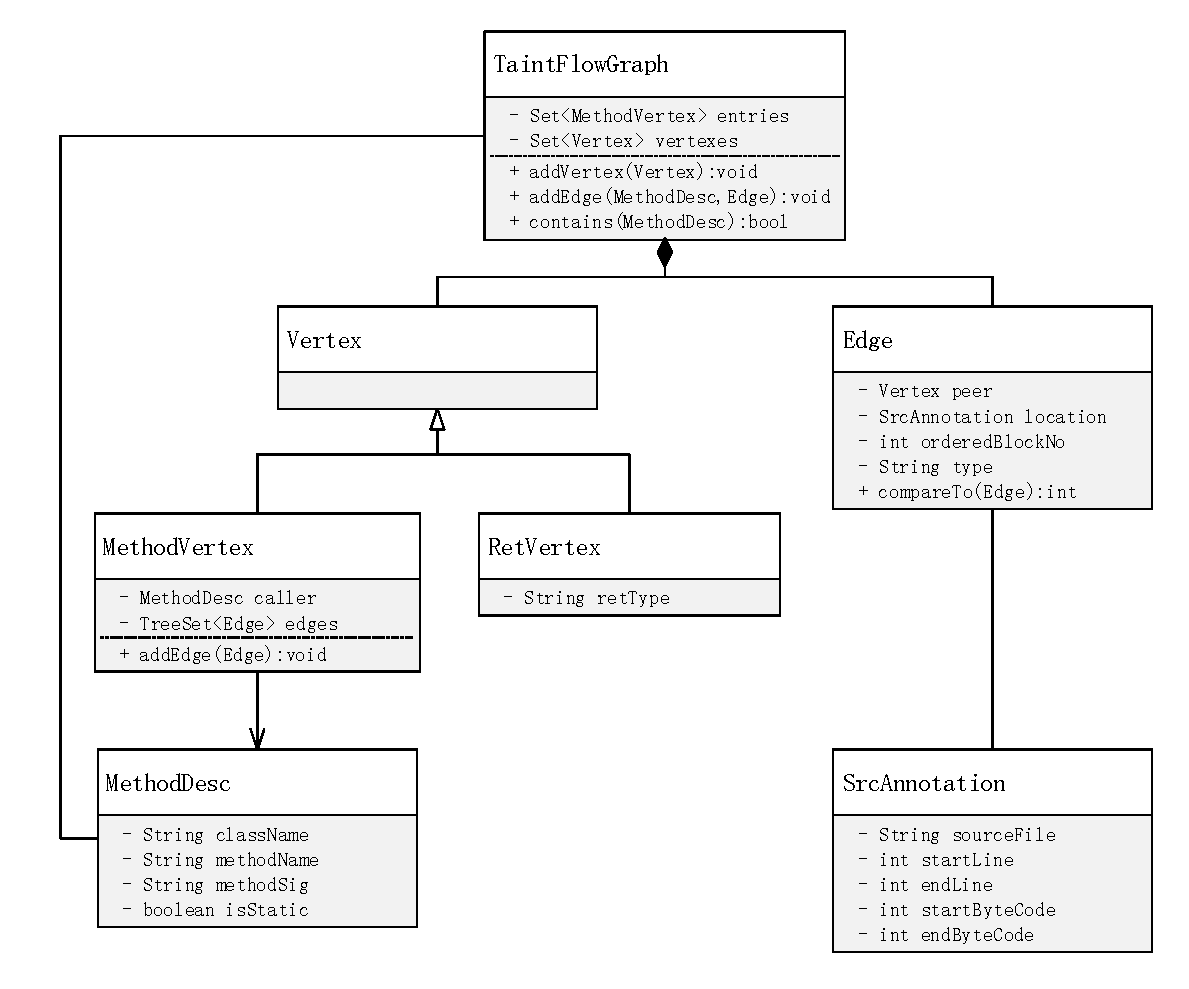
\includegraphics[width=0.8\textwidth]{FIGs/chapter3/taintGraphClass.pdf}
	\caption{污点传播图设计}\label{taintGraphClass}
\end{figure}

类 TaintFlowGraph 代表了一张污点传播图,图上的点由 Vertex 类表示,边由 Edge 类表示。TaintFlowGraph 中 entries 属性表示这张图入口函数的集合,这些函数只有出度没有入度,换句话说,污点在这些函数的上下文中传入,并传播至图中其他点,通常来说,这些函数有Web应用的视图层函数(如继承 \textit{HttpServlet} 子类中的 \textit{doGet()} 或 \textit{doPost()} 方法)或是客户端程序的入口函数(如 \textit{main()} 函数),该类中有向图中增加点的方法 \textit{addVertex()} 和向图中增加边的方法 \textit{addEdges()},还有一个检查函数摘要是否存在于图中的方法 \textit{contains()}。函数摘要类 MethodDesc 在系统逻辑视图中已出现过,该类主要用来唯一标识类中的函数,含有属性 className、methodName、methodSig 和 isStatic,分别表示类名,方法名,函数签名和是否为静态类。

顶点类 Vertex是一个抽象类,具体派生出表示函数的函数顶点类 MethodVertex 和 返回指令顶点类 RetVertex,MethodVertex 包含了一个函数摘要 caller ,以及该函数内连向其他顶点的边 edges,并且包含添加边的方法 \textit{addEdge()}。返回指令顶点类表示函数体中返回污点变量的返回值语句,其属性只有该语句类型 retType——通常来说 Java字节码 返回语句有 \textit{ireturn},\textit{dreturn},\textit{areturn} 等。不难发现,污点传播图上的顶点为函数或返回语句,并且只有 MethodVertex 才可以有出度,所以,在 TaintFlowGraph 类中的 \textit{addEdge()} 方法表示顶点的参数只能是一个函数摘要类型的顶点。

最后设计与边相关的类,Edge 类,该类表示这一条边和连接这一边的对端顶点,peer 属性表示对端顶点, location 代表了两点之间通过哪一个代码位置与之相连,type 指这条边的类型,模块中主要有三种类型(“CALL”,代表函数调用;“SINK”,代表调用到汇聚点,“RET”,代表函数返回),blockId 属性表示这条边所在的代码块,该属性的目的是为了结合 CFG 将污点传播图拆解为传播树,以及保证边的顺序。代码位置有SrcAnnotation 该类将在下一章详细说明。\\

% 是否要举个例子或者话一张该图的数据结构?

\subsection{污点传播树和漏洞报告类图设计}

污点传播树是展示污点传播过程的重要数据结构,其中叶子结点中有一污点入口点和一污点汇聚点,其他叶子节点为函数或返回语句节点,树的层级关系反映出函数调用关系,一棵传播树代表了一个唯一的污点传播全流程,其结构体和漏洞报告类图设计如图~\ref{taintTreeAnnotationClass}所示。

对于污点传播树,有一工具类TaintTreeGenerator,主要有两个方法:\textit{makeTree()} 和 \textit{makeAnnotation()},\textit{makeTree()} 方法输入为污点传播图的一个入口点,根据这一入口点构造若干棵传播树;\textit{makeAnnotation()}根据污点传播树构造出一注解列表,这些注解列表最终在GUI界面上展现污点传播树。

考虑到污点传播树存在树形结构,并且节点存在运行顺序的上下关系的特征,本模块设计使用树的孩子兄弟结构来表示污点传播树。TreeNode 表示树上节点对象,其 id 表示了该节点的序号,其主要用来在反序列化时重构树;location 属性表明了该节点在程序中的位置,type 表示节点类型,在本系统中,该类型种类和传播图的 Edge 类型一致;firstChild 为 TreeNode 对象,指向其第一个子节点,具体来说,父节点是一个函数节点,而子节点可以使函数节点或是返回节点;nextSib 为 TreeNode 对象,指向同一深度的下一个叶子对象,具体地说,是同一函数上下文下的下一对象。TreeNode 派生出两类节点,一个是表示函数的节点 MethodTreeNode,其有一类型为 MethodDesc 的属性 caller,另一个是表示返回语句的节点 RetTreeNode,其有一属性 retType 表示了返回语句类型,与上文 RetVertex 类型一致。

% 是否要举个例子或者画一张该图的说明该注解还以?
漏洞注解类 BugAnnotation 、漏洞实例 BugInstance 类和漏洞实例 BugCollection 类都是 Spotbugs 定义的数据类型,漏洞注解类该类表示了对漏洞的一行解释性文字。
BugInstance 是应用中一个漏洞的基本单位,其有一个漏洞类型(type 属性)和多行漏洞注解(list 属性)组成。在 BugAnnotation 中, \textit{format()} 是该条注解在GUI界面上的显示文字时被调用的方法,\textit{writeXML()} 用于将注解保存为XML格式,以上为原生 Spotbugs 定义的方法,除此之外,为了方便反序列化,本模块还为其增加了 \textit{fromXML()}方法。NoteAnnotation、RetNodeAnnotation 和 MethodNodeAnnotation 对应于污点传播树的 TreeNode、RetTreeNode 和 MethodTreeNode 节点,对于抽象的节点注解类 NoteAnnotation 而言,其id、firstId,nextId 分别指向了 TreeNode的id,第一个孩子节点的id和第一个兄弟节点的id,depth 表示该节点距离树根的深度,具体类 RetNodeAnnotation 和 MethodNodeAnnotation 会将重现实现 BugAnnotation 类的三个方法,特别的,RetNodeAnnotation 的 firstId 恒为-1,因为返回语句的节点不会存在子节点。BugCollection类主要有漏洞实例组成,除此之外,其还记录有项目名称,用户提交的应用jar包(appJars)、依赖包(libJars)和源码包(srcs)。


\begin{figure}[!htb]
	\centering
	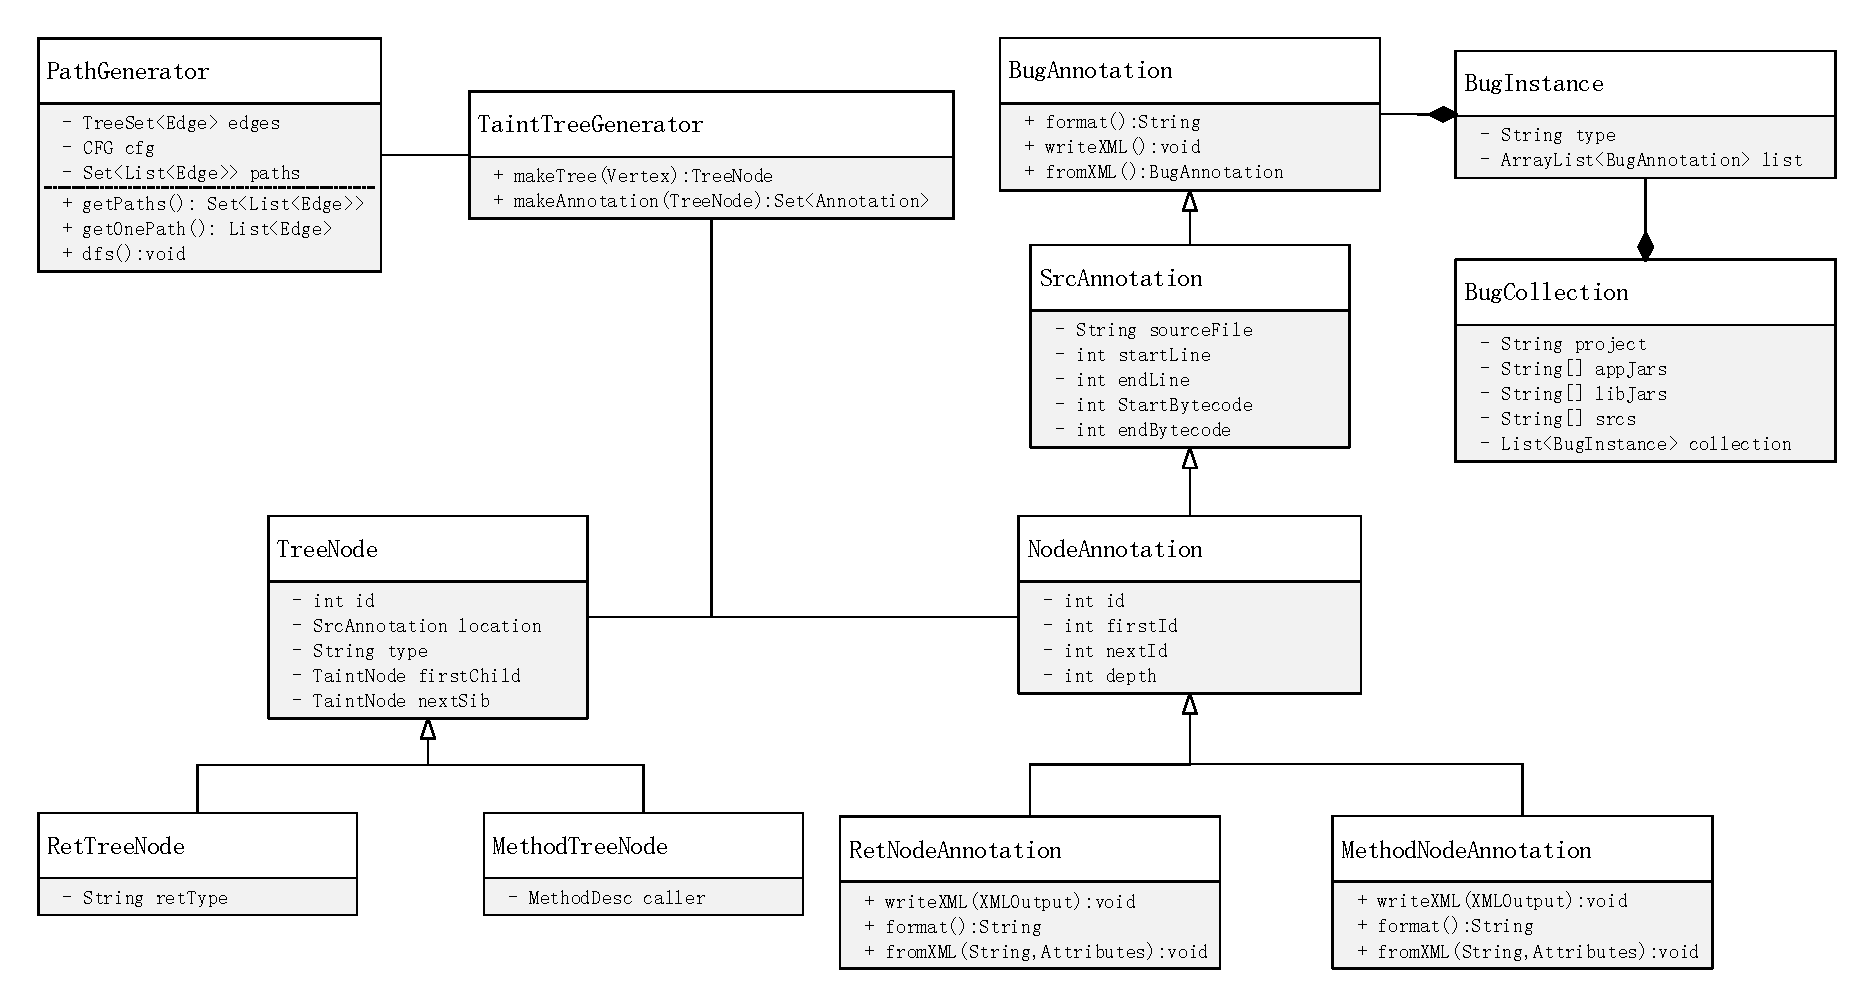
\includegraphics[width=0.8\textwidth]{FIGs/chapter3/taintTreeAnnotationClass.pdf}
	\caption{污点传播树和漏洞报告类图设计}\label{taintTreeAnnotationClass}
\end{figure}

\subsection{污点分析器类图设计}

污点分析器类图设计如图~\ref{taintDetectorClass}所示,Detector 类是所有分析器的基类,对于每一个 Detector 子类,Spotbugs会按流程图~\ref{taintprocess}所示使其分析目标 Jar 中的每个类,其中调用的就是类中 \textit{visitClassContext()} 方法,类遍历完成后,又会调用 \textit{report()} 方法产生报告。
\begin{figure}[!htb]
	\centering
	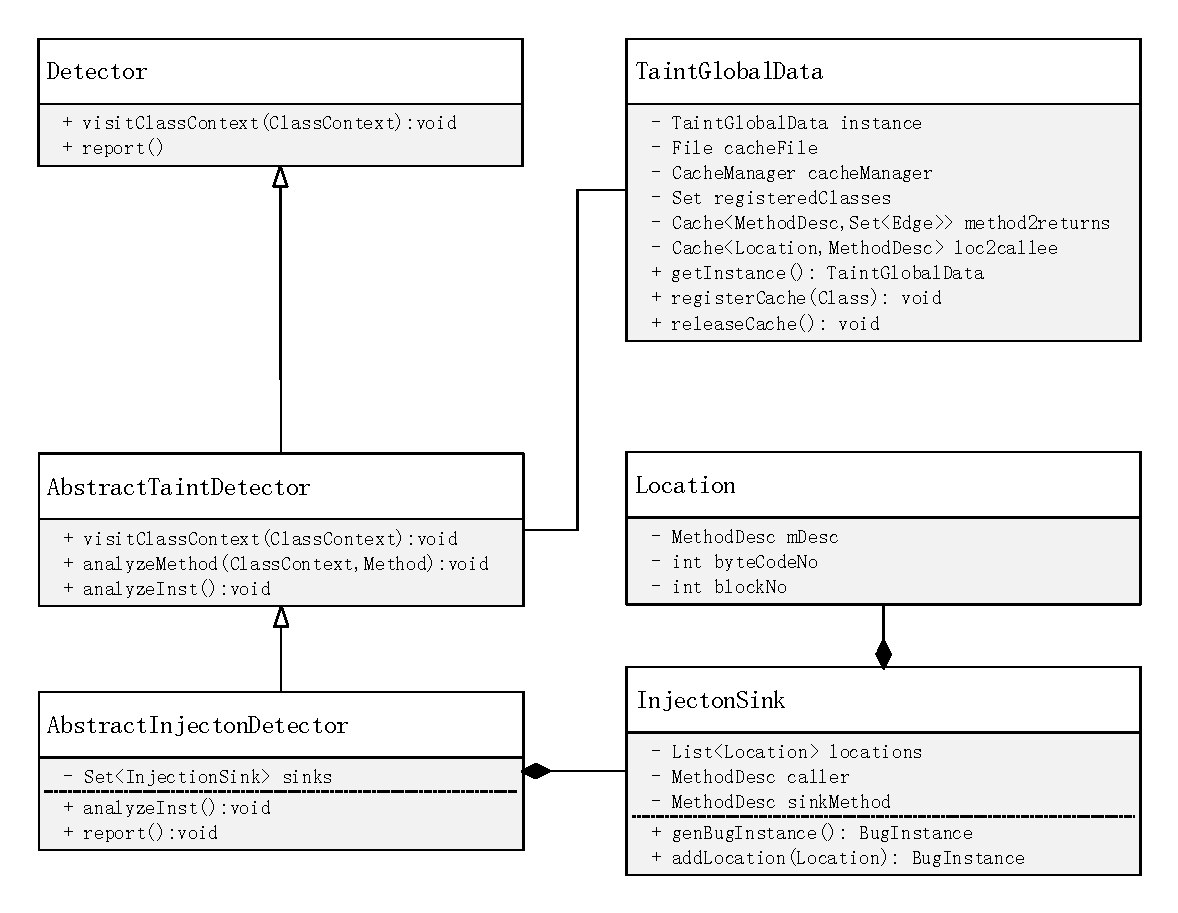
\includegraphics[width=0.8\textwidth]{FIGs/chapter3/taintDetectorClass.pdf}
	\caption{污点分析器类图设计}\label{taintDetectorClass}
\end{figure}

AbstractTaintDetector 继承 Detector 类,该类也是记录污点传播信息的重要基类,其关键在于 returns 属性和 loc2callee 属性,returns记录了每一个函数中能够返回污点变量的 return 语句,loc2callee 记录了在函数调用发生时,invoke指令所在的函数位置和被调用的函数摘要。其会实现 Detector 的 \textit{visitClassContext()} 方法,并且在该方法内,调用 \textit{analyzeMethod()} 方法对每一个目标函数进行分析,对于污点传播信息的记录逻辑也在该方法内。对于特殊指令,如 \textit{return} 和 \textit{invoke},\textit{analyzeMethod()} 会调用  \textit{analyzeInst()} 对指令进行分析。

AbstractInjectionDetector 继承了 AbstractInjectionDetector,进一步实现了污点分析过程,即实现了 \textit{analyzeInst()} 和 \textit{report()} 方法,其属性 sinks 记录了目标应用的所有汇聚点,在所有类的分析完成后,依次调用 \textit{report()} 生成报告。

污点汇聚点的类名为 InjectionSink,其属性 caller 和 sinkMethod 为调用敏感函数的最后一个函数,以及敏感函数的函数摘要,除此之外,所有将污点汇聚到该点的调用语句有被记录在其 locations 列表上,\textit{addLocation()} 就是记录调用语句发生位置的方法,\textit{getBugInstance()} 方法为产生报告的具体方法,被 \textit{AbstractInjectionDetector.report()} 方法调用,构造污点传播图、传播树和生成漏洞实例逻辑都在该方法中。

上面提到的位置信息由 Location 类表示,其包含的属性有语句所在函数的函数摘要(mDesc),语句所在的字节码序号(byteCodeNo)和所在 CFG 代码块的序号(orderedBlockNo)。



\section{程序切片模块设计}

程序切片模块是误报预测的基础,本系统优化了前人工作,能够对一个漏洞进行完整切片,本节从流程设计类图设计两方面介绍该模块的设计。\\
\subsection{流程设计}

本模块的流程设计如图~\ref{sliceProcessing} 所示,该模块的输出是用户提交的项目 Jar 包和在上一模块已经产生的漏洞报告中的漏洞实例集合,其输出是切片项目类,从类图分析可知,该项目类中含有所有漏洞及对应的所有切片。

\begin{figure}[!htb]
    \centering
    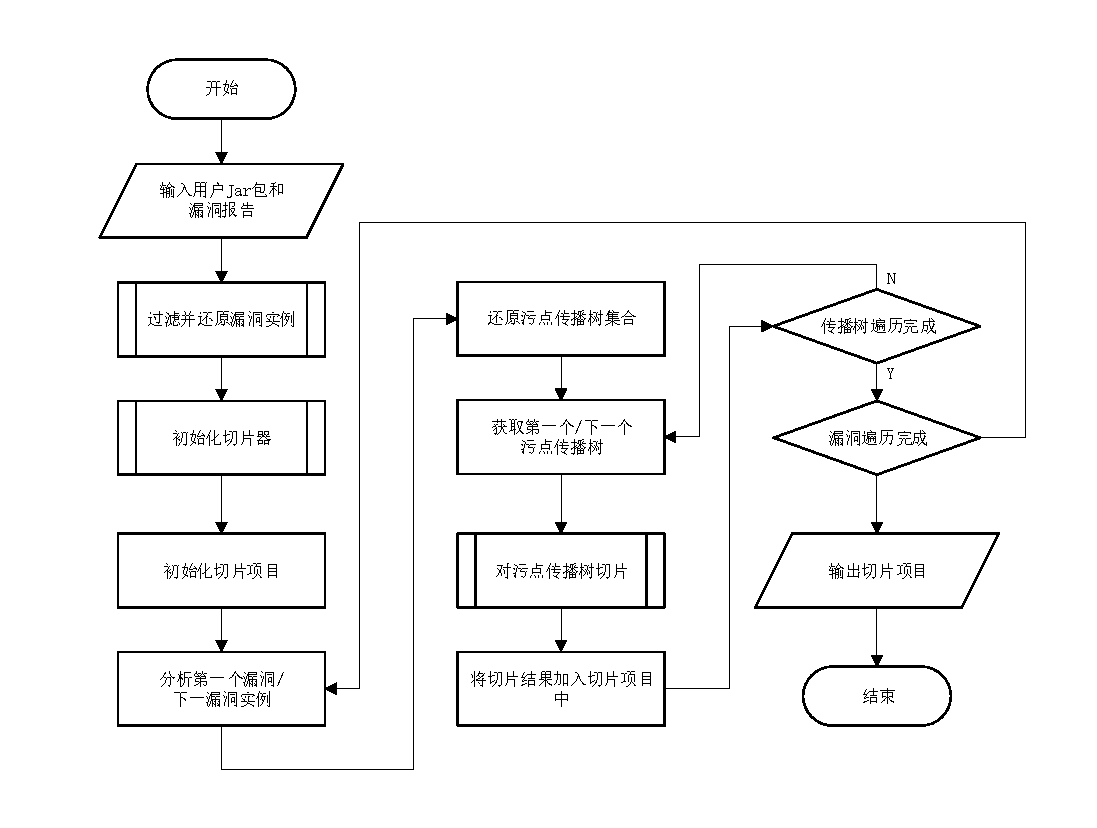
\includegraphics[width=0.8\textwidth]{FIGs/chapter3/sliceProcessing.pdf}
    \caption{程序切片模块流程图}\label{sliceProcessing}
\end{figure}

因为 Spotbugs 中除了上文提到的污点传播检测器还存在其他漏洞检测器,其他检测器产生漏洞不属于本系统处理范围,在模块运行前,先要对漏洞报告进行过滤,同时将污点传播类型的漏洞反序列化漏洞注解,接着模块初始化一个具体的程序切片器,其中包括了对切片器的各种配置,具体会在实现章节介绍,以及初始化一个空的切片项目。接下来将会遍历漏洞实例集合中的每一个漏洞,对于一个污点传播漏洞,根据上一模块产生的漏洞实例注解集,还原出若干棵污点传播树,接下来就是对污点传播树进行拆解并切片的步骤,该步骤是本系统的核心步骤之一,包括了对污点传播树进行拆解,将其分为污点传播流作为为更小的切片任务,其具体实现也将在下一实现章节介绍;对污点传播树的切片结束后,将传播树信息和对应切片集合加入项目中,遍历完所有漏洞的污点传播树后,模块输出切片项目,项目内存在与漏洞相关的所有切片。\\

\subsection{类图设计}

\begin{figure}[!htb]
    \centering
    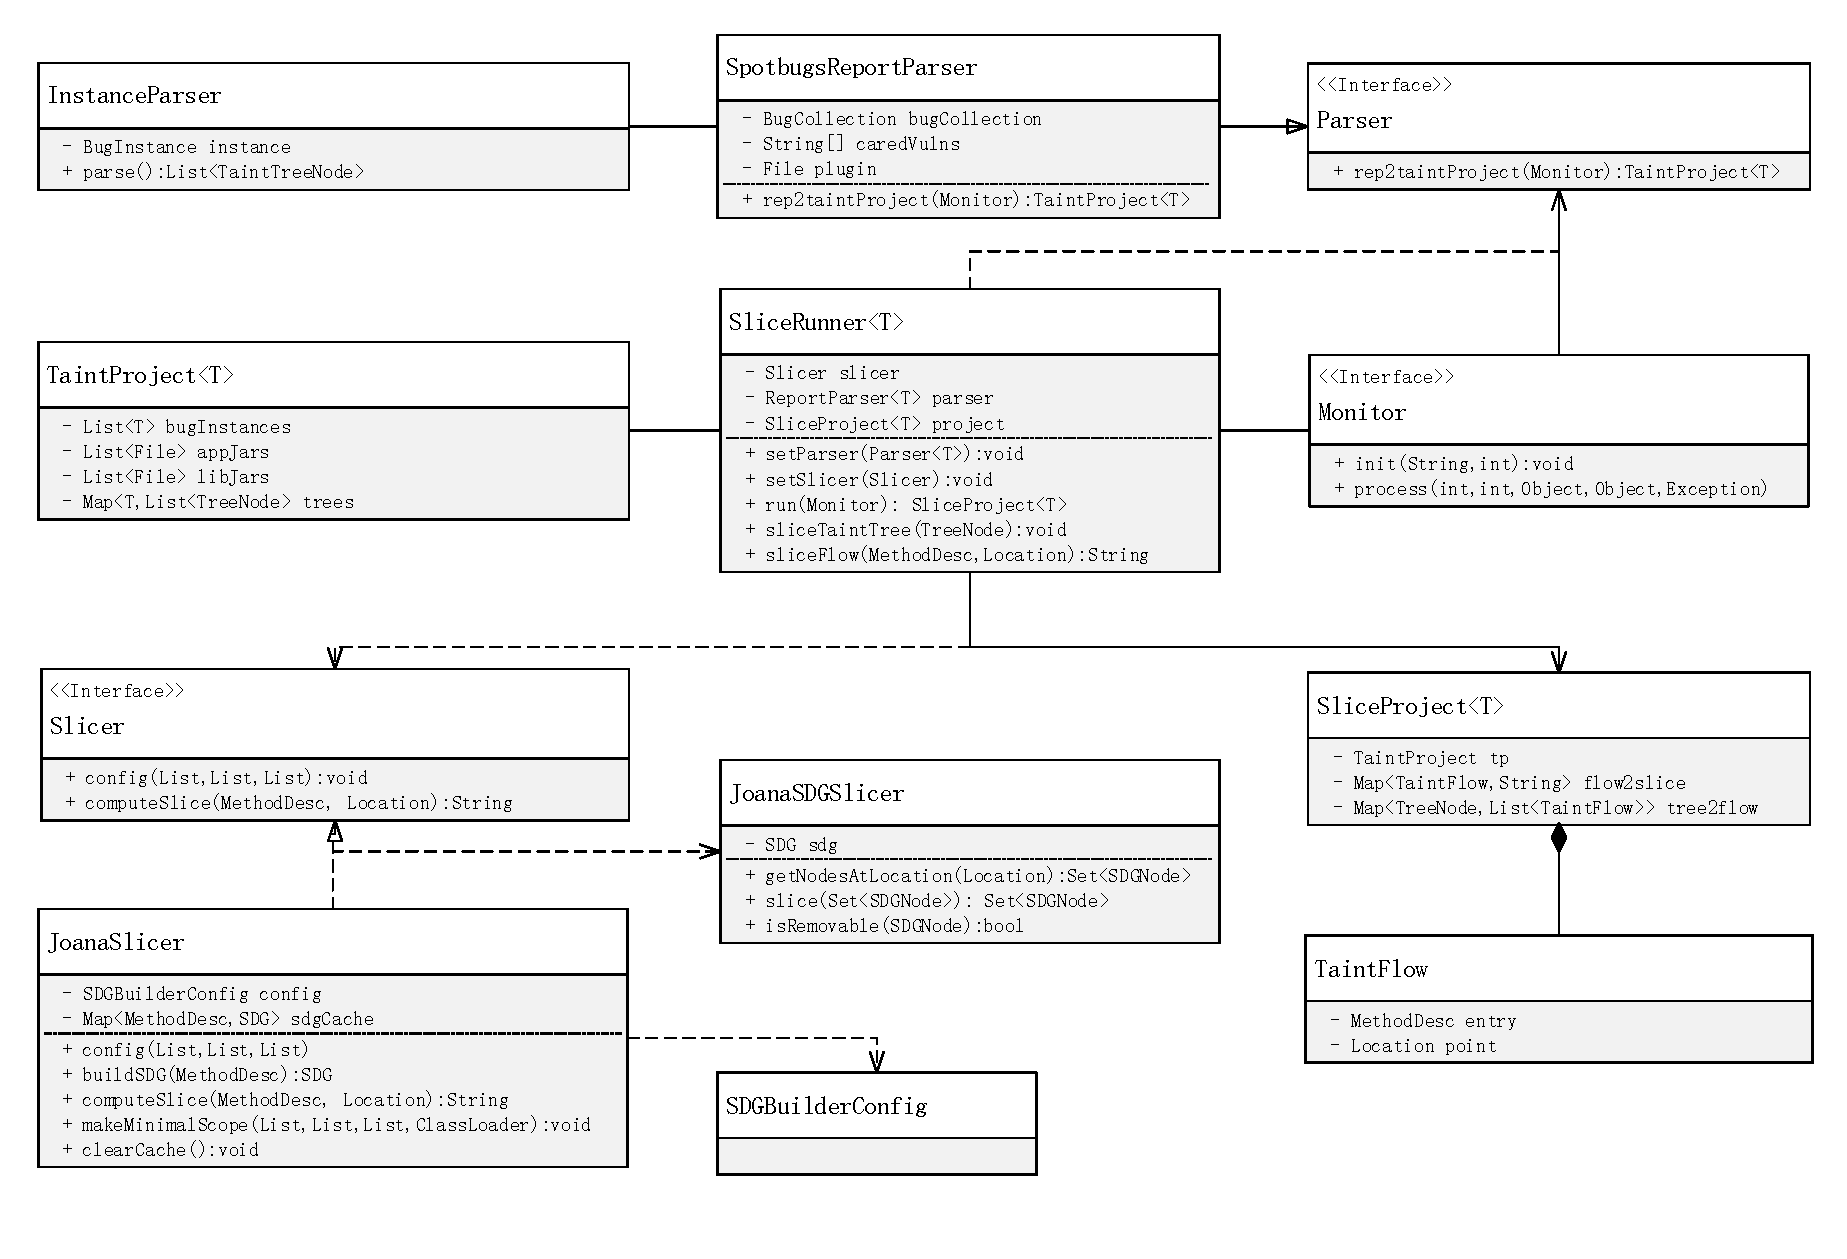
\includegraphics[width=0.9\textwidth]{FIGs/chapter3/sliceClass.pdf}
    \caption{程序切片模块类图}\label{sliceClass}
\end{figure}

本模块的类图设计如图~\ref{sliceClass} 所示。首先介绍模块的核心控制类 SliceRunner,该类用于读取污点传播报告,并最终产生每一漏洞实例的切片集合,其有三个属性成员:slicer,表示用于切片的切片器;parser,污点传播报告的翻译器;project,最终输出的切片项目。切片器和翻译器分别由 \textit{setSlicer()} 和 \textit{setParser()} 设置,\textit{run()} 方法是对漏洞报告切片的控制方法,其参数是一个监视器,上一章节所说的模块流程将在该方法内完成,\textit{sliceTaintTree()} 是对一个污点传播树切片的方法,可以看到其参数是一个树节点表示该传播树的树根,\textit{sliceFlow()} 是对一个传播流切片的方法。

Monitor 类是监视器接口,用于方便各种耗时较长的函数中间返回信息,具体地说,该接口的 \textit{init()} 方法用于通知类开始某一流程,第一个参数为过程名,第二个参数表示过程共几个子过程;\textit{process()} 方法用于在每一个子过程完成后调用,其参数依次向监视器发送了当前子过程序号,过程总数,子过程输入,子过程输出,以及遇到的异常。该接口规范了系统内的任务进度报告模式,使外部能够自由的处理每一子过程并及时通知用户(例如,在每一子过程完成时向屏幕输出进度或是处理异常),除了切片控制类会使用该类外,未来的预测控制类也会使用。

接下来设计与污点传播翻译器相关的类,Parser 是翻译器接口,其 \textit{rep2taintProject()} 方法用来将漏洞报告翻译为一个污点传播项目,同样,其也有一个监视器作为参数。 SpotbugReportParser 实现了该接口,其属性有 bugCollection,该属性在类初始化时传入,表示污点传播报告,caredVulns 表示污点传播漏洞类型白名单,该属性为静态属性,plugin 为本系统优化后的 FindSecBugs 插件(注意到反序列化函数 \textit{fromXML()} 在插件中)。SpotbugReportParser 的 parse() 方法将漏洞报告转化为了污点传播项目,而真正将漏洞实例还原为若干棵污点传播树的是来自 InstanceParser 类中的 \textit{parse()} 方法,该类成员变量 instance 为一漏洞实例,在类构造时传入。翻译的最终产出是 TaintProject 对象实例,该类中 bugInstances 表示了所有的污点传播方法,appJars 和 libJars 表示了用户提交的应用 Jar 包集合和第三方依赖 Jar 包集合,trees 为一组键值对,记录了一个 bugInstance 的所有污点传播树的树根节点。

Slicer 是切片器的接口,\textit{config()} 方法用来配置一个切片器,其中三个列表参数分别代表引用 Jar 包,第三方依赖 Jar 包和黑名单类,当切片内容在黑名单类的上下文时,该条切片被舍弃,这主要用来过滤 Java Runtime 中的切片,或者排除其他第三方包的切片。\textit{computeSlice()} 方法是对一个污点传播流的切片方法,其参数是指以 MethodDesc 的函数为入口进行对关注点 Location 的切片,切片返回String类型,每条切片用“$\backslash$n”分割。 JoanaSlider 类是 Slicer 的一个具体实现,其 config 变量表示一个用于保存生成SDG 的配置信息,配置类名为 SDGBuilderConfig,由于该类涉及到实现细节,将在下一章进行讨论, sdgCache 用于缓存SDG,类中除了实现 \textit{config()} 和 \textit{computeSlice()} 方法,还有构造 SDG 的方法 buildSDG(),其参数为 SDG 的入口函数的函数摘要,\textit{makeMinimalScope()} 方法为构造最小搜索范围方法,被构造 SDG 时使用,clearCache() 方法用于清除各类缓存,在构造 SDG 后,主要切片工作由 JoanaSDGSlicer 梳理,该类在创建时传入 SDG 作为属性,先通过 \textit{getNodesAtLocation()} 获取关注点的 SDGNode,再通过 \textit{slice()} 方法切出所有相关的 SDGNode,并且通过 \textit{isRemovable()} 函数将一些无效节点删除(如非函数语句节点,抽象类节点等)。

切片模块最终返回切片项目类 SliceProject 对象,该对象内部持有一污点传播项目对象,从传播树到污点传播流的映射(tree2flow 属性)和从污点传播边到切片的映射(edge2slice 属性)。TaintFlow 对象代表污点传播流,可以看到,其属性 entry 和 point 正好对应了切片器接口切片函数的参数,它的实际上代表了污点在一个函数内传播的过程。

从本模块的类图设计上可以看出,本模块基本上实现了对切片器和污点分析器的解耦,在某些类上的泛型 T 表示了漏洞类型类,考虑到了今后不同污点分析工具的返回漏洞类型不同这一情况,即使今后需要换用其他污点分析引擎或是切片器,只需要重新实现 Parser 和 Slicer 再修改泛型就可重用本模块。

\section{数据预处理模块设计}
\subsection{类图设计}
\subsection{流程设计}

\section{误报预测模块设计}
\subsection{架构设计}
\subsection{类图设计}
\subsection{流程设计}

\section{数据库设计}
本系统的数据库主要用来存储用户身份信息、污点分析得到的污染流数据和标记、用于模型训练的参数配置信息以及模型本身信息。经过分类,可以总结为三类数据表:

第一类是与鉴权有关的数据表,由于本系统主要使用了C/S架构,为了防止恶意攻击者向服务器注入垃圾数据影响预测,因此需要对客户端身份进行鉴定,为此设立客户端口令(Client\_Token)表,由安全运营人员进行维护。

第二类是与程序分析相关的数据表,由于本系统后台主要是对子污染流的切片进行有监督预测,因此自然需要污染流(Taint\_Flow)表和对污染流的标记(Label)表,对一个污染流而言,需要对其函数入口和关注点(即语句位置)进行切片,因此存在函数摘要(Method\_Description)表和语句位置(Location)表,不同项目可能具有名称相同的类、函数或文件,为了在逻辑上唯一标识一个函数摘要和语句位置,因此建立项目(Project)表。

第三类是与模型本身相关的数据表,本系统使用BLSTM进行切片预测,对BLSTM训练和BLSTM结构本身涉及到一系列参数,为此将其保存在模型配置(Model\_Config)表中,供安全运营人员调整,对于已经训练好的模型,将其保存在BLSTM模型(LSTM\_Model)表中。

与鉴权有关的数据表实体关系图如图~\ref{er:token} 所示,其中只有一张表,即客户端口令表,其中字段如表~\ref{sql:tokenTable} 所示,id 为一个口令的唯一标识;token 为一字符串,由管理员设置和发放,客户端连接时需要有一合法 token 才可与服务器通信;description 用于保存该口令的一些描述信息;create\_time 为该口令的创建时间。
\begin{figure}[!htbp]
	\centering
	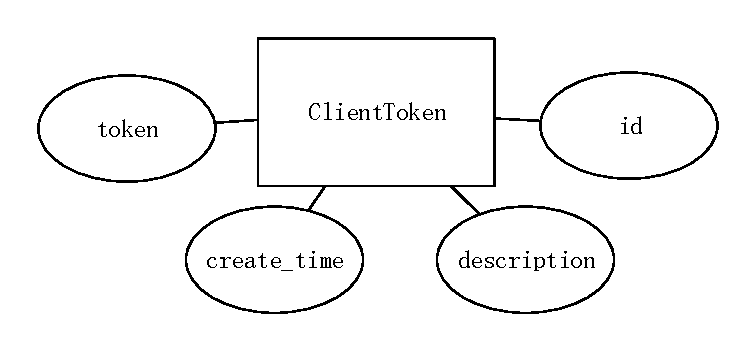
\includegraphics[width=0.5\linewidth]{FIGs/chapter3/token_er.pdf}
	\caption{与鉴权相关表的实体关系图}\label{er:token}
\end{figure}

\begin{table}[!htbp]\footnotesize %token table
	\centering
	\caption{Client\_Token 表}
	\vspace{2mm}
	% l - left, r - right, c - center. | means one vertical line 这里声明的是表格单元中的内容如何对齐
	\begin{tabular}{L{2cm}L{2cm}L{2.6cm}L{6cm}}
		\toprule
		\textbf{字段名}&\textbf{数据类型}&\textbf{属性}&\textbf{说明}\\
		\midrule
		id					&INT&PK&主键,token的唯一标识\\
		token 				&VARCHAR(255)&NN, UNIQUE&表示管理员向用户发放的 token\\
		description				 &VARCHAR(255)& N &用于保存管理员对此 token 的备注信息\\
		create\_time		  &DATETIME&NN&表示 token 的创建时间\\
		\bottomrule
	\end{tabular}
	\label{sql:tokenTable}
\end{table}

与程序分析相关的实体关系图如图~\ref{er:program},其中,项目表保存项目名称,函数摘要表保存一个项目中的函数摘要信息,语句位置表记录关注点所在的代码位置,污染流表记录污染流和其中的切片信息,标记表记录一个污染流记录是否是安全的。一个项目可以有多个函数摘要、位置和污染流,即有一对多的关系,一个函数摘要或语句位置可以有多个污染流记录,而标记和污染流记录呈一对一关系。

\begin{figure}[!htbp]
	\centering
	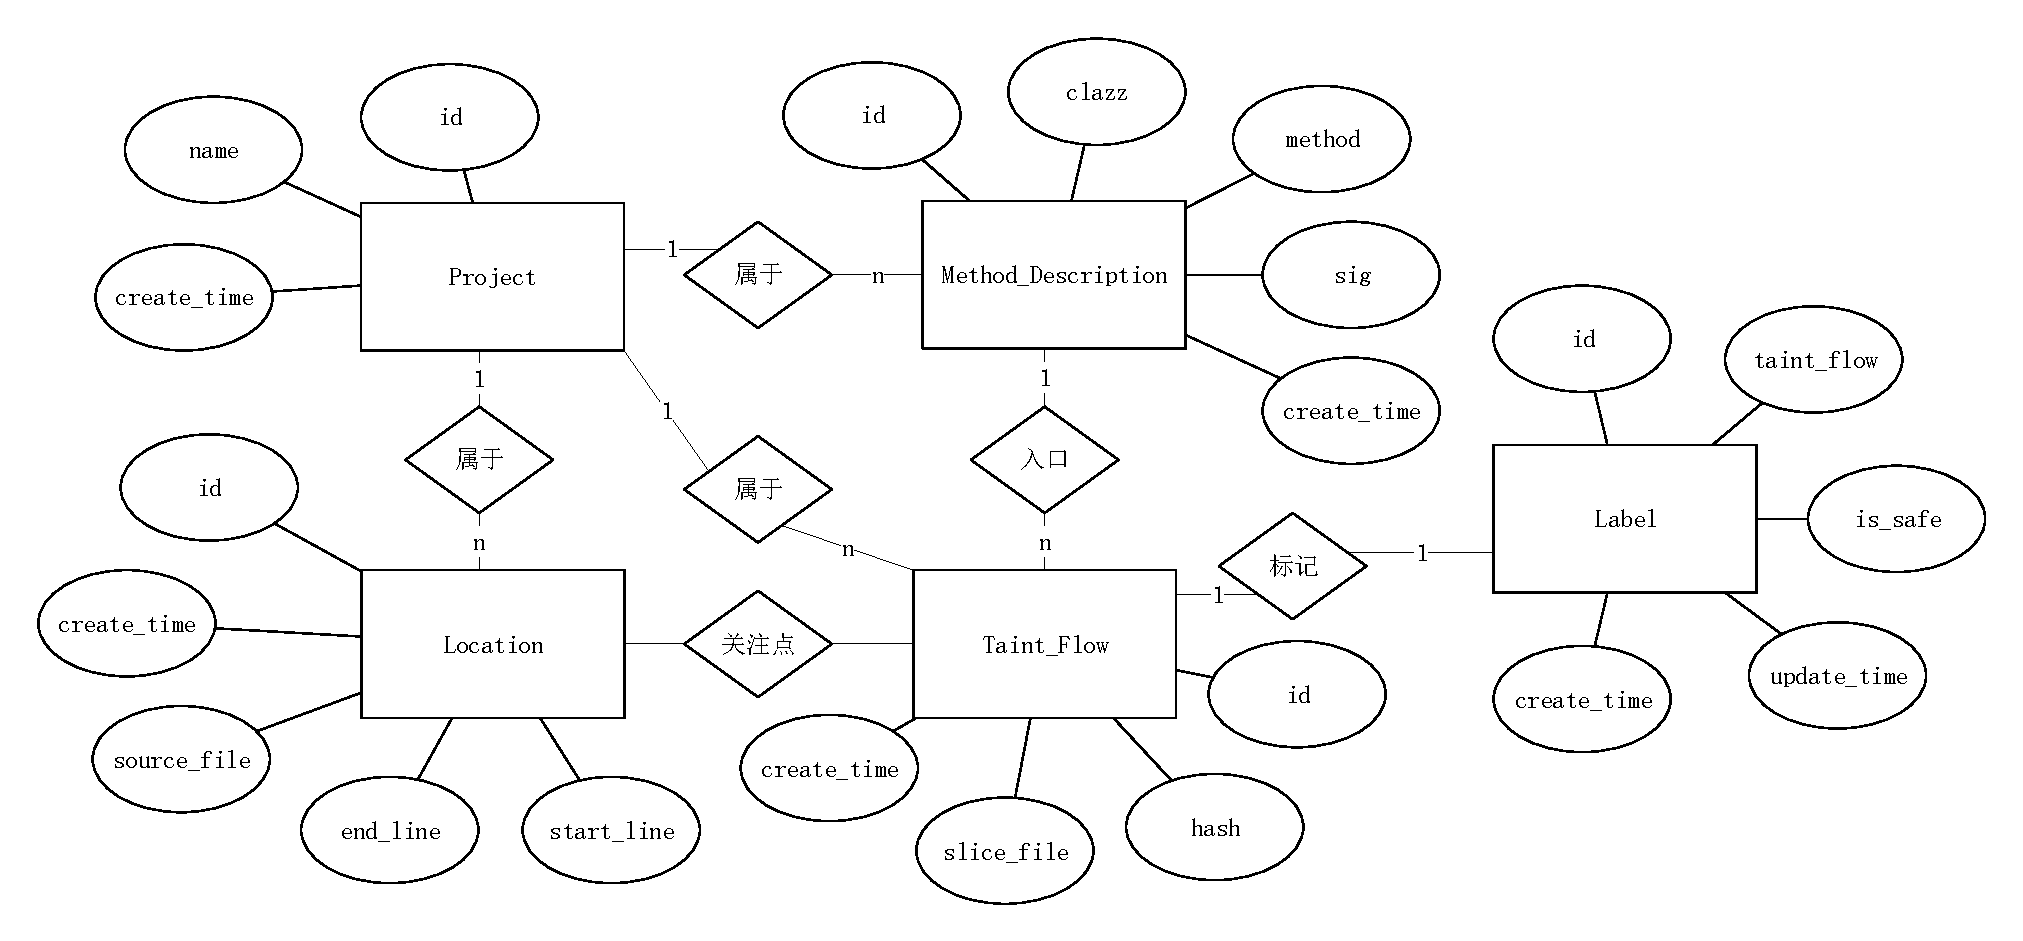
\includegraphics[width=1\linewidth]{FIGs/chapter3/program_er.pdf}
	\caption{与程序分析相关表的实体关系图}\label{er:program}
\end{figure}

表~\ref{sql:project}是对项目表的字段说明,其中,id是一个项目的唯一标识;name标识项目名称,存在唯一性约束,由客户端建立扫描项目时指定;create\_time记录该项目的创建时间。

\begin{table}[!htbp]\footnotesize %project table
	\centering
	\caption{Project 表}
	\vspace{2mm}
	% l - left, r - right, c - center. | means one vertical line 这里声明的是表格单元中的内容如何对齐
	\begin{tabular}{L{2cm}L{2cm}L{2.6cm}L{6cm}}
		\toprule
		\textbf{字段名}&\textbf{数据类型}&\textbf{属性}&\textbf{说明}\\
		\midrule
		id							&INT&PK&主键,项目的唯一标识\\
		name		 			&VARCHAR(255)&NN&表示项目的名称\\
		create\_time		  &DATETIME&NN&表示项目创建时间\\
		\bottomrule
	\end{tabular}
	\label{sql:project}
\end{table}

表~\ref{sql:methodDescription}是对函数摘要表的字段说明,其中,id 是一个函数摘要的唯一标识;clazz 记录函数的类名;method 记录函数的方法名;sig 记录函数签名,其包括了参数类型和返回值类型;project 作为外键,标识该函数摘要位于哪个项目中;create\_time记录该函数摘要的创建时间。此外,clazz,method,sig,project能够唯一标识一个函数摘要。
\begin{table}[!htbp]\footnotesize %methodDescription table
	\centering
	\caption{Method\_Description 表}
	\vspace{2mm}
	% l - left, r - right, c - center. | means one vertical line 这里声明的是表格单元中的内容如何对齐
	\begin{tabular}{L{2cm}L{2cm}L{2.6cm}L{6cm}}
		\toprule
		\textbf{字段名}&\textbf{数据类型}&\textbf{属性}&\textbf{说明}\\
		\midrule
		id					&INT&PK&主键,函数摘要的唯一标识\\
		clazz				&VARCHAR(255)&NN&表示该函数的类名\\
		method 			& VARCHAR(255) &NN&表示该函数的方法名\\
		sig					&VARCHAR(255)&NN&表示该函数的签名,即函数参数和返回值类型\\
		project  		  &INT&FK, NN&外键,指向Project,表示该函数出现在此项目中\\
		create\_time  &DATETIME&NN&表示标记创建时间\\
		\bottomrule
	\end{tabular}
	\label{sql:methodDescription}
\end{table}

表~\ref{sql:location}是对语句位置表的字段说明,其中,id是一个语句位置的唯一标识;source\_file记录该语句所在的文件名	;start\_line记录该位置开始的代码行号;end\_line记录该位置结束的代码行号  ;project作为外键,记录该位置位于哪个项目中;create\_time记录该项目的创建时间。此外,source\_file,start\_line,end\_line,project联合可以唯一标识一个语句位置。
\begin{table}[!htbp]\footnotesize %location table
	\centering
	\caption{Location 表}
	\vspace{2mm}
	% l - left, r - right, c - center. | means one vertical line 这里声明的是表格单元中的内容如何对齐
	\begin{tabular}{L{2cm}L{2cm}L{2.6cm}L{6cm}}
		\toprule
		\textbf{字段名}&\textbf{数据类型}&\textbf{属性}&\textbf{说明}\\
		\midrule
		id							&INT&PK&主键,语句位置的唯一标识\\
		source\_file		 	&VARCHAR(255)&NN&表示语句所在文件名\\
		start\_line 			& INT &NN, UNSIGNED&表示语句所在的开始行号\\
		end\_line				&INT&NN, UNSIGNED&表示语句所在的结束行号\\
		project  			  &INT&FK, NN&外键,指向Project,表示该位置出现在此项目中\\
		create\_time		  &DATETIME&NN&表示标记创建时间\\
		\bottomrule
	\end{tabular}
	\label{sql:location}
\end{table}

表~\ref{sql:taintFlow} 是对污染流表的字段说明,其中,id 是一个污染流的唯一标识;hash	是这个污染流的哈希,通过切片文本的SHA1得到;slice\_file 切片文件在硬盘上的保存位置,当数据库中记录删除时,切片文件也应被删除;entry和point分别为切片的入口点和关注点 ;project作为外键,记录污染流存在于哪个项目中;create\_time记录该污染流的创建时间。此外,entry,point和project可以联合唯一标识一个污染流记录。

\begin{table}[!htbp]\footnotesize %taintFlow table
	\centering
	\caption{Taint\_Flow 表}
	\vspace{2mm}
	% l - left, r - right, c - center. | means one vertical line 这里声明的是表格单元中的内容如何对齐
	\begin{tabular}{L{2cm}L{2cm}L{2.6cm}L{6cm}}
		\toprule
		\textbf{字段名}&\textbf{数据类型}&\textbf{属性}&\textbf{说明}\\
		\midrule
		id					&INT&PK&主键,污染流的唯一标识\\
		hash				&VARCHAR(255)&NN&表示污染流的哈希\\
	    slice\_file			& VARCHAR(255) &NN&表示污染流切片的文件名\\
		entry				&INT&FK&外键,指向Method\_Description,表示污染流切片的入口\\
		point				&INT&FK&外键,指向Location,表示污染流切片的结束位置\\
		project  		  &INT&FK, NN&外键,指向Project,表示污染流所在的项目\\
		create\_time  &DATETIME&NN&表示污染流的创建时间\\
		\bottomrule
	\end{tabular}
	\label{sql:taintFlow}
\end{table}

表~\ref{sql:label}是对标记表的字段说明,其中,id 是一个标记的唯一标识;taint\_flow 作为外键,指这被标记的污染流对象,同时一个污染流同时只能有一个标记;entry和point分别为切片的入口点和关注点 ;is\_safe 标记了该污染流是安全/不安全的;create\_time记录该标记的创建时间;update\_time记录该标记的更新时间。

\begin{table}[!htbp]\footnotesize %label table
	\centering
	\caption{Label 表}
	\vspace{2mm}
	% l - left, r - right, c - center. | means one vertical line 这里声明的是表格单元中的内容如何对齐
	\begin{tabular}{L{2cm}L{2cm}L{2.6cm}L{6cm}}
		\toprule
		\textbf{字段名}&\textbf{数据类型}&\textbf{属性}&\textbf{说明}\\
		\midrule
		id							&INT&PK&主键,标记的唯一标识\\
		taint\_flow		 		&INT &FK, NN&外键,指向Taint\_Flow,表示本标记的污染流对象\\
		is\_safe 				& BOOLEAN &NN&表示这个污染流是安全的\\
		create\_time		  &DATETIME&NN&表示标记创建时间\\
		update\_time		&DATETIME&NN&表示标记更新时间\\
		\bottomrule
	\end{tabular}
	\label{sql:label}
\end{table}

与模型相关的实体关系图如图~\ref{er:model} 所示,其中,模型配置(Model\_Config)表记录模型配置信息,主要包括了配置名,模型训练相关信息和 LSTM 模型的参数等,LSTM 模型表(LSTM\_Model)记录以训练好的模型信息,主要信息有训练度量,模型保存位置等,一个配置可以训练多个模型。

\begin{figure}[!htbp]
	\centering
	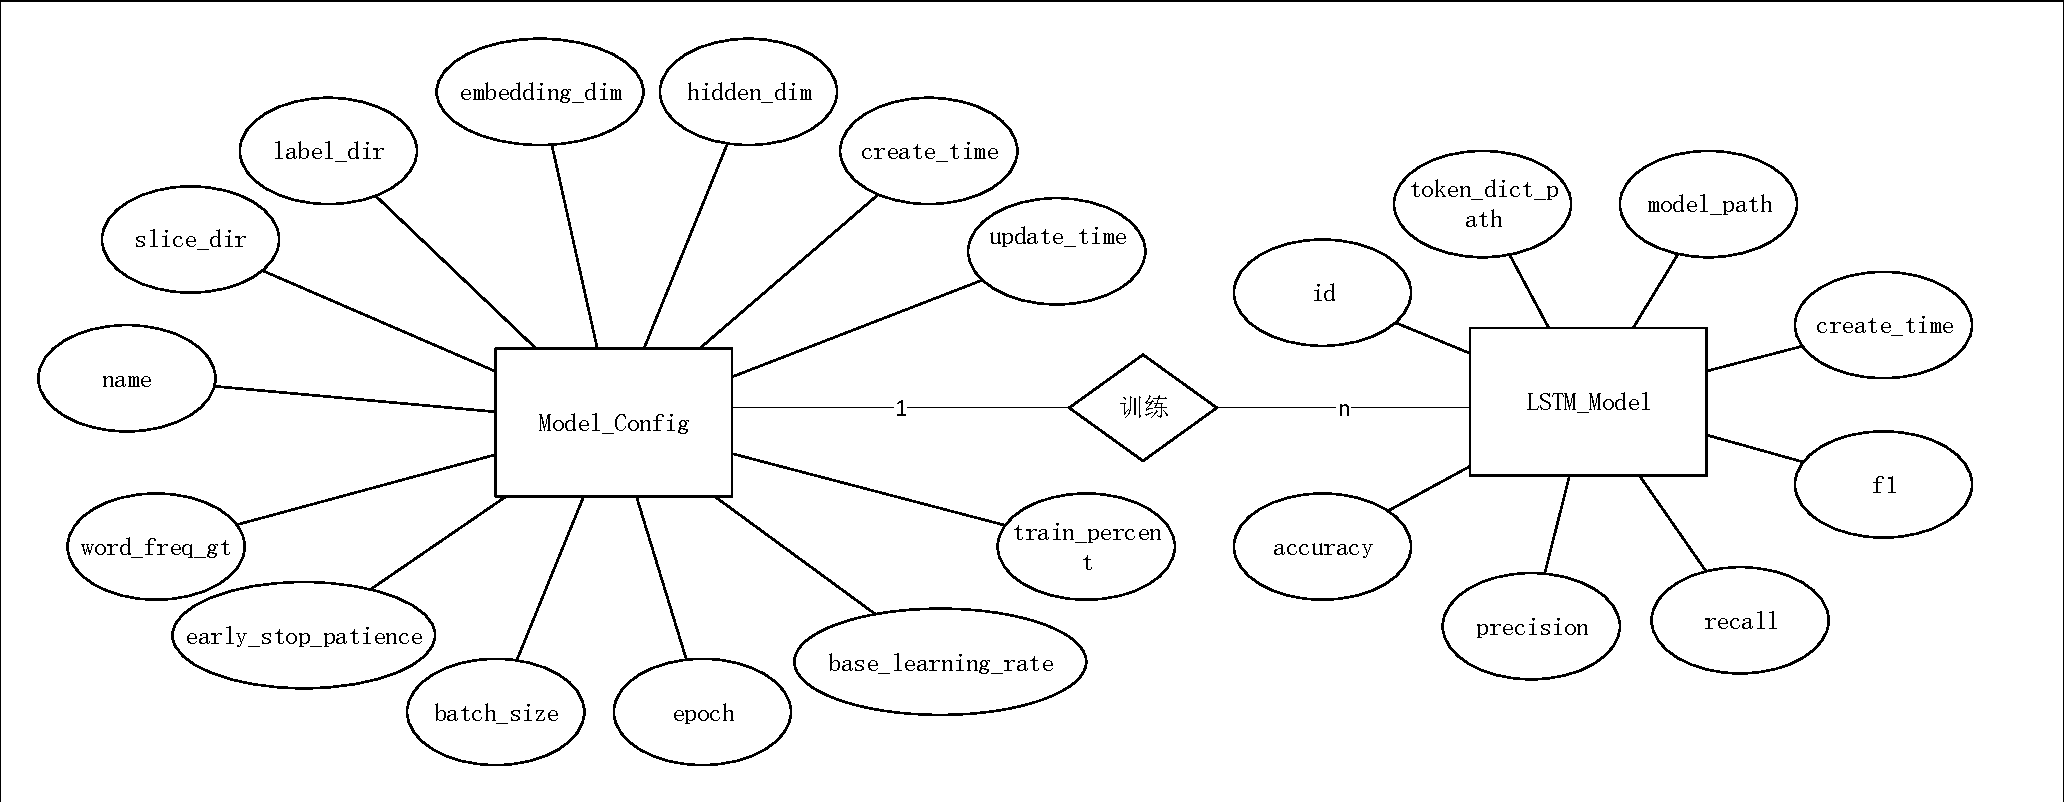
\includegraphics[width=1\linewidth]{FIGs/chapter3/model_er.pdf}
	\caption{与模型相关表的实体关系图}\label{er:model}
\end{figure}

 表~\ref{sql:modelConfigTable} 是对模型配置表的字段说明,其中 name 作为主键,用于唯一标识一个配置,训练时通过指定改值进行训练;slice\_dir 和 label\_dir 记录了学习用的数据集位置,分别表示了切片所在文件夹和标记所在文件夹(模型直接通过文件进行读取,而不从数据库读取,减少了IO消耗);embedding\_dim,hidden\_dim 为模型自身参数,分别代表词嵌入的维度和隐藏层神经元个数(模型的每层神经元个数相等);word\_freq\_gt 表示了将出现次数小于该值的单词表示为“UNK”(Unknown);early\_stop\_patience,base\_learning\_rate,batch\_size,epoch,train\_percent记录了模型训练的配置,early\_stop\_patience 值训练轮数超过改值后,若模型效果(loss)仍比之前最优效果差,则提前停止训练,base\_learning\_rate 指初始学习率,batch\_size 指批量传入模型的数据量,epoch 指最大训练轮数,train\_percent 指训练集占总数据集的百分比,剩下的数据作为训练集,用于评估训练效果;最后,create\_time 和 update\_time 分别表示配置创建时间和配置更新时间。

\begin{table}[!htbp]\footnotesize %model config table
	\centering
	\caption{Model\_Config 表}
	\vspace{2mm}
	% l - left, r - right, c - center. | means one vertical line 这里声明的是表格单元中的内容如何对齐
	\begin{tabular}{L{2.2cm}L{2cm}L{2.6cm}L{6cm}}
		\toprule
		\textbf{字段名}&\textbf{数据类型}&\textbf{属性}&\textbf{说明}\\
		\midrule
		name 						&VARCHAR(255)&PK&主键,唯一标识一个配置\\
		slice\_dir		 			&VARCHAR(255)&NN&模型使用切片数据所在的文件夹\\
		label\_dir		 			&VARCHAR(255)&NN&模型使用标记数据所在的文件夹\\
		embedding\_dim		  &INT&NN, UNSIGNED&词嵌入时的维度,值为正整数\\
		hidden\_dim				&INT&NN, UNSIGNED&隐藏层神经元的个数,值为正整数\\
		word\_freq\_gt			&INT&NN, UNSIGNED&最小词频,小于该词频则表示为UNK,值为正整数\\
		early\_stop\_patience		&INT&NN, UNSIGNED&提前停止忍耐度,如果学习轮数大于此值,效果仍比以前差则学习停止,值为正整数\\
		base\_learning\_rate		&DOUBLE&NN, UNSIGNED&初始学习率\\
		batch\_size					&INT&NN, UNSIGNED&批量数据记录数,每次向神经网络输入batch\_size条记录,再进行反向传播\\
		epoch						&INT&NN, UNSIGNED&训练最大迭代次数,超过该次数则停止训练\\
		train\_percent						&DOUBLE&NN, UNSIGNED&表示训练集占整个数据的百分比,默认为1,即将所有数据代入训练\\
		create\_time				&INT&NN, UNSIGNED&配置创建时间\\
		update\_time				&INT&NN, UNSIGNED&配置更新时间\\
		\bottomrule
	\end{tabular}
	\label{sql:modelConfigTable}
\end{table}

表~\ref{sql:lstmModelTable} 是对 BLSTM 模型表的字段说明,其中 id 作为主键唯一标识一个模型;token\_dict\_path 和 model\_path 分别表示单词到整形值的映射字典文件位置和BLSTM模型位置,这两个字段用于加载模型实现对切片的预测;config 表示模型是由何配置训练得到的;accuracy、precision、recall和F1表示了模型的四种度量,当配置划分没有训练集时,这些值为-1;create\_time记录模型被训练出的时间。

\begin{table}[!htbp]\footnotesize %lstm model table
	\centering
	\caption{BLSTM\_Model表}
	\vspace{2mm}
	% l - left, r - right, c - center. | means one vertical line 这里声明的是表格单元中的内容如何对齐
	\begin{tabular}{llll}
		\toprule
		\textbf{字段名}&\textbf{数据类型}&\textbf{属性}&\textbf{说明}\\
		\midrule
		id&INTEGER&PK&主键,模型的唯一标识\\
		token\_dict\_path &VARCHAR(255)&NN&保存单词到tokenid的字典文件位置\\
		model\_path		 &VARCHAR(255)&NN&保存BLSTM模型文件的位置\\
		config				 &VARCHAR(255)&FK,NN&指向Model\_Config表,表示模型对应的配置信息\\
		accuracy	&DOUBLE&NN&表示学习后训练集的准确率,若无训练集则为-1\\
		precision	&DOUBLE&NN&表示学习后训练集的精确率,若无训练集则为-1\\
		recall	&DOUBLE&NN&表示学习后训练集的召回率,若无训练集则为-1\\
		F1	&DOUBLE&NN&表示学习后训练集的F1,若无训练集则为-1\\
		create\_time		  &TIME&NN&记录模型创建时间\\
		\bottomrule
	\end{tabular}
	\label{sql:lstmModelTable}
\end{table}

\section{本章小结}

\chapter{Java静态安全扫描系统实现和测试}
\section{一个XSS漏洞实例}
为了说明扫描系统的实现,本小节将首先介绍一段简单的 XSS 漏洞Java Web代码,在接下来的几个小节中都将使用该代码辅助说明模块实现。

\begin{minipage}[!htbp]{0.9\textwidth}
\lstinputlisting[language=Java, caption={一段含XSS漏洞的Java代码}, label={code:xss}]{FIGs/chapter4/xssDemo.java}
\end{minipage}

代码如~\ref{code:xss} 所示,类 XSS 继承 HttpServlet,因此其可以通过重写 \textit{doGet()} 和 \textit{doPost()} 方法向用户提供HTTP服务,在 doGET 方法中,其从用户输出参数 \textit{p} 中获取值,接着判断值,若值以“safe”开头,则 \textit{q} 被赋值为 \textit{safe(p)},否则 \textit{q} 被赋值为 \textit{unsafe(p)},最终通过 \textit{sink()} 方法向用户返回 \textit{q},在 \textit{doPOST()} 方法中,其直接调用 \textit{safe()} 方法,并将其返回。分析 \textit{safe()} 和 \textit{unsafe()} 方法不难发现,\textit{safe()} 方法是一个典型的过滤方法,而 \textit{unsafe()} 方法则存在安全性问题,这也造成 \textit{doGet()} 方法存在安全性问题,而 \textit{doPost()} 不存在安全问题。

\section{污点分析模块的实现}\label{sec:taintImp}
\subsection{污点分析时记录污点传播信息实现}
在污点分析模块的设计章节中,提到了要想输出带有污点传播树信息的漏洞实例报告,必须在污点分析函数时记录函数内部信息,具体来说就是函数调用语句位置信息和函数返回位置信息。本小节将结合伪代码和具体事例,说明这一部分的实现。

\begin{algorithm}[!htb]\footnotesize
\caption{记录污点传播信息算法实现}
\label{alg:noteTaint}
\KwIn{$method$,函数上下文信息 }
\KwOut{$R$, 返回语句位置集合;$I$, 调用语句位置集合;$T$, 于污点传播相关语句位置集合}
$mDesc \leftarrow getDesc(method)$\\
$R \leftarrow \varnothing $\\
$I \leftarrow \varnothing $\\
$T \leftarrow \varnothing $\\
$initTaint \leftarrow -1$\\
$dataflow \leftarrow getDataflow(method)$;\\
\ForEach {block in dataflow} {
    \ForEach {location in block} {
        $inst \leftarrow location.getInst()$\\
        \If {initTaint = -1} {
            $initTaint \leftarrow dataflow.getFact(location).getNum()$\\
        }
        \If {inst is ReturnInst} {
            $currTaint \leftarrow dataflow.getFact(location).getNum()$;\\
            \If {currTaint \textgreater initTaint} {
                $edge \leftarrow buildEdge(location, inst)$\\
                $R \leftarrow R \cup \left\{ \left\langle mDesc, edge \right\rangle \right\}$\\
            }
        }
        \ElseIf {inst is InvokeInst} {
            $callee \leftarrow inst.getCallee()$;\\
            $I \leftarrow R \cup \left\{ \left\langle location, callee \right\rangle \right\}$\\
            $analyzeLocation(method, location, inst)$\\
            \If {sink influenced by invoke}{
                $T \leftarrow T \cup \left\{ location \right\}$\\
            }
        }
    }
}
\end{algorithm}

伪代码~\ref{alg:noteTaint} 说明了函数内记录传播信息的实现,该算法以一个函数的上下文信息 method 为输入,输出函数内返回语句的位置集合 $R$、调用语句位置集合 $I$ 和与污点传播相关语句位置集合 $T$ 。显然,实际的该算法实现在 \textit{AbstractTaintDetector.analyzeMethod()} 方法中,并且 $R$ 和 $I$ 实际上可以用 Map 类型记录,在函数内的$R$、$T$ 和 $S$ 会加入到类中的对应全局集合中。

1-6 行为算法初始化阶段,包括获取函数的函数摘要,初始化算法输出集合 $R$、$I$和$T$,将函数初始被污染的参数个数 $initTaint$ 设为 -1(表示初始值还未设置),以及获取当前函数的数据流图。接下算法通过两层遍历,按数据流图顺序遍历每一个代码块中的每一条语句位置,在循环体中,首先根据语句位置获取语句内容,当$initTaint$未设置值时,将其赋值为获取第一条语句时的污染个数,通常该值小于等于该函数的参数个数(污点传播到一个或多个函数实参上)。

若当前语句时一个返回值调用语句,由于一个函数内可能有若干条返回语句,并且返回语句未必会返回可能携带污点的变量,不传播污点的返回语句不需要记录在 $R$ 中,例如在代码片段~\ref{code:xss} 中,函数 \textit{unsafe()} 就存在两条返回语句,然而,第 25 行的返回语句并不可能传播污点,因此 25 行并不需要记录。 判断语句是否传播污点的方法是判断当前语句的传播的污点数量是否比刚进入时的污点数量多(根据FindSecBugs污点分析方法,即使函数原样返回实参,污点个数也会比初始值多1)。

若语句是一条调用语句,首先通过该语句获取被调用的函数摘要,将当前位置和函数摘要一并放入 $I$ 中,不难看出 $I$ 实际上记录了该类的函数调用图,再做函数调用间分析,该分析已由原生 FindSecBugs 实现,这里不再赘述,根据分析结果判断汇聚点是否可以被当前函数调用影响,则向$T$中加入这一位置,以代码片段为例,当分析到第 8 行时,因为先前分析过 \textit{safe()} 可以传播污点(函数分析按调用图的拓扑排序进行),即 p 污点传播到了 q,又因为污点 \textit{q} 作为参数流入了汇聚点 \textit{sink()},即根据污点传播结果发现汇聚点受到这次调用的影响,便将第 8 行加入 $T$ 中,同理,被加入 $T$的还有第 5 行(污点入口点)、第 9 行、第 11 行和第 12 行。\\

\begin{minipage}[!htbp]{0.9\textwidth}
    \lstinputlisting[language=Java, caption={构造污点传播图的实现}, label={code:taintGraph}]{FIGs/chapter4/taintGraph.java}
\end{minipage}\\

\subsection{构造污点传播图实现}
\vspace{0.7cm}
在得到返回语句位置集合、调用语句位置集合和污点传播相关语句位置集合后,可以构造污点传播图,其构造方式如代码~\ref{code:taintGraph} 所示,实际存在于 \textit{InjectionSink.genBugInstance()} 方法中。\\

首先,代码构造了一个空的污点传播图,将直接调用敏感函数的边加入图中,以代码~\ref{code:xss} 为例,将$sink() \rightarrow Writer.write()$ 加入图中;接着向图中添加相关函数调用的边(12-19 行),具体地说,遍历污点传播相关语句位置集合,对于每一个 location,获取其调用函数(location 记录了调用函数的函数摘要),再获取其被调用函数(只需查找调用语句位置集合 loc2callee 即可),随后在将 location 转化为 SourceLineAnnotation,将生成一条边并加入图中即可; 最后,向图中加入返回语句的点和边(21-27 行),只需要遍历先前得到的返回语句位置集合(injDetector.returns)即可。\\

\subsection{构造污点传播树实现}

在得到污点传播图后,对图的每一入口进行深度优先搜索,得到污点传播树集合,搜索算法~\ref{alg:buildTaintTree}所示,算法实现于 \textit{TaintTreeGenerator.makeTree()} 函数中。\\

\begin{algorithm}[!htb]\footnotesize
    \caption{构造污点传播树伪代码实现}
    \label{alg:buildTaintTree}
    \KwIn{$v$,污点传播图的一个入口,$getCFG()$,获取当前函数的CFG}
    \KwOut{$trees$, 污点传播树根的集合}
    \SetKwProg{Fn}{Function}{}{}
\Fn{dfs(u: MethodVertex, e: Edge, isSource: bool): Set<TreeNode>}{
    $trees \leftarrow \varnothing$\\
    $paths \leftarrow getPaths(u, u.edge, getCFG(u.caller), isSource)$\\
    \ForEach {path in paths} {
        $pathTrees \leftarrow \varnothing$\\
        $pathTrees \leftarrow pathTrees \cup \{node(u, e)) \} $\\
        $i \leftarrow 0$\\
        \ForEach {edge in path}{
            \If{edge.peer is MethodVertex}{
                $subTrees \leftarrow dfs(edge.peer, edge, false)$\\
                $newPathTrees \leftarrow \varnothing$\\
                \For{tree in pathTrees}{
                    \For{subTree in subTrees}{
                        $newTree \leftarrow tree$\\
                        $addNode(newTree, subtrees, i)$\\
                        $newPathTrees \leftarrow newPathTrees \cup \{newTree\}$
                    }
                }
                $pathTrees \leftarrow newPathTrees $\\
            }
            \Else{
                \For{tree in pathTrees}{
                    $leaf \leftarrow node(edge.peer, edge)$\\
                    $addNode(tree, leaf, i)$\\
                }
            }
            $i \leftarrow i+1$\\
        }
        
        $trees \leftarrow trees \cup pathTrees$\\
    }
    \Return{trees}\\
}
$trees \leftarrow dfs(v, null,true)$\\
\end{algorithm}

搜索函数即 $dfs()$,其参数有函数 u 、调用 u 的污点传播边(若入口函数则置空)以及是否为入口函数,输出该函数 u 的污点传播树集合。

函数初始化返回的树集合 trees,由于传播树的代表了污点传播的一条路径,因此根据函数 u 的 CFG 遍历出所有程序执行路径,即 \textit{getCFG()} 函数,在该函数中,还需根据函数性质去除不符合要求的路径,如在污点入口函数处,路径上的第一个节点必须为污点入口点,若函数包含连向污点汇聚点的边,那么路径上必须包含该边。

遍历每一条执行路径,接着建立当前路径上的传播树集合 pathTrees,初始化为空,并且将当前函数入口 u 所在节点作为树根加入集合中,用 i 表示路径序号。遍历路径上出现的污点传播边,若边的对端顶点是一个函数类型的点,则新建一个传播树集合 newPathTrees 并递归获取其子传播树集合,下面两层循环遍历当前传播树将其加上其子传播树后产生新的传播树,将其加入 newPathTrees 中,最后用新的树集合代替原先集合(第 12-20 行)。这一列的操作本质在于,pathTrees的树个数代表了当前路径的路径数 n,而 subTrees 中树的个数代表了函数内有的路径树 m,那么执行完该函数后,总的路径数应该是 $n \times m$,即 newPathTrees 中树的个数。若边的对端顶点是一个返回值顶点,则直接生成叶子节点并将其加入树中。
$addNode(tree, subtree, i)$函数用于将子树加入主树的第一层树干中,若$i=0$将其加入至孩子节点,否则将其加入至最后一个兄弟节点后。

对于入口函数 v(注意,该入口函数不是第二章介绍的污点入口点,而是图上没有入度的点,实际上的污点入口点发生在 v 节点代表的函数中),调用$dfs(v, null,true)$ 即可返回函数入口的多个污点传播树。

上述算法也说明了,一个入口之所以有多个污点传播树,其根本原因是污点传播路径不同,例如代码~\ref{code:xss} 中的 \textit{doGet()} 函数,搜索后,可以得到如图~\ref{taintTree} 所示的两棵污点传播树。

\begin{figure}[!htb]
    \centering
    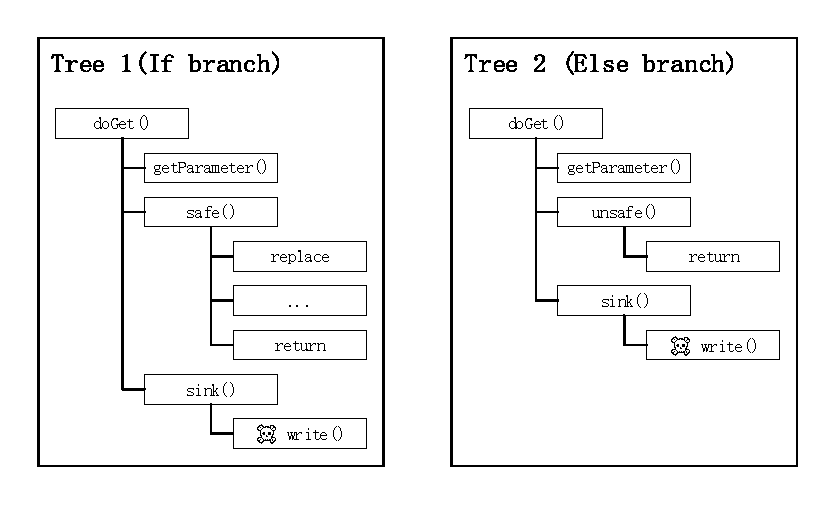
\includegraphics[width=0.9\textwidth]{FIGs/chapter4/taintTree.pdf}
    \caption{\textit{doGet()} 函数的污点传播树}\label{taintTree}
\end{figure}


得到污点传播树后,对传播树再做一次深度搜索可以将书上的所有节点转化为可以显示在界面上的注解,其算法表示如下:

\begin{algorithm}[!htb]\footnotesize
    \caption{构造污点传播树注解伪代码实现}
    \label{alg:buildAnnotation}
    \KwIn{$n$,污点传播树树根;$depth$,树节点深度,初始化为0;$book$以处理的位置,初始化为$\varnothing$;$annotations$,当前注释集合,初始化为$\varnothing$}
    \KwOut{$R$, 污点传播树的注解集合}
    \SetKwProg{Fn}{Function}{}{}
    \Fn{dfs(n:TreeNode, depth: int, book: Set<SrcAnnotation>, annotations: Set<SrcAnnotation>) : Set<SrcAnnotation> }{
        \If{n is null}{
            \Return{$\varnothing$}
        }
        \If{n in book}{
            \Return{$\varnothing$}
        }
        $R \leftarrow annotations \cup \left\{ getAnnotation(n) \right\} $\\
        $R \leftarrow R \cup dfs(n.firstChild, depth+1, book \cup \{n.location\}, annotations)$\\
        $R \leftarrow R \cup dfs(n.nextSib, depth, book \cup \{n.location\}, A)$\\
        \Return{R}
    }
\end{algorithm}

对于污点传播树的搜索比传播图要简单的多,只要先将当前节点构造成,搜索其孩子节点和兄弟节点即可,注意兄弟孩子节点可能为空,因此在搜索前需要判断,若为空值则返回空集,此外,通过算法~\ref{alg:buildTaintTree} 构造的树节点实际上是存在回路的,在打印时需要考虑到这点,因此增加了 book 参数记录,限制当前节点不能延树干向上搜索。在一开始调用时,只需要将 depth 设为 0,book 和 A 设为空集即可。

对于污点传播图的每一个入口函数,可以构造一至多棵污点传播树,对应的就有一至多组注解集合。

\section{程序切片模块的实现}
在设计章节,本文已经对该模块的功能,主要流程和重要类图进行了介绍,在本节中,将从后向切片和整个流程的控制模块两方面具体介绍该模块的具体实现。\\

\subsection{切片控制模块实现}

\subsubsection{切片控制代码}

切片控制模块的实现代码片段如代码~\ref{code:sliceControl} 所示,该代码出现在 SliceRunner 的 run() 方法中,主要功能是调用翻译器和切片器对一个目标项目中的所有漏洞切片,即执行流程图~\ref{sliceProcessing} 上的流程。

代码的第1行首先调用 reportParesr 将项目进行过滤和翻译,得到 taintProject, 接着第三行通过项目中的应用 Jar 包和依赖 Jar包,对 slicer 进行配置。接着遍历污点传播类型的漏洞实例,对于每一个实例,获取其污点传播树集合(第11行),接着遍里污点传播树,对每一个污点传播树进行切片(第19行),每完成一个漏洞实例后向监视器汇报进度(第24-25行),并且若是 Joana 类型的切片器,对切片器进行清除缓存的操作,防止缓存过多造成 OOM,最后返回切片项目。\\

\vspace{-0.7cm}
\begin{minipage}[!htbp]{0.9\textwidth}
    \lstinputlisting[language=Java, caption={切片控制模块实现代码片段}, label={code:sliceControl}]{FIGs/chapter4/sliceControl.java}
\end{minipage}
\vspace{0.7cm}

\subsubsection{过滤漏洞实例}
本系统实现了切片预测逻辑和污点传播逻辑的解耦,从而产生了翻译漏洞报告这一过程。在 Spotbugs 报告类型的翻译器中,主要逻辑在于对漏洞过滤并还原污点传播树。对于污点传播树的还原可以通过对漏洞注解的二次遍历实现,这里不再赘述,本节主要通过代码~\ref{code:sliceFilter},介绍过滤漏洞实例的实现。

\begin{minipage}[!htbp]{0.9\textwidth}
    \lstinputlisting[language=Java, caption={漏洞过滤代码片段}, label={code:sliceFilter}]{FIGs/chapter4/sliceFilter.java}
\end{minipage}

从第 3-4 行可以看出,模块按漏洞类型过滤掉了非污点传播类型漏洞、已经修复的漏洞(在 Spotbugs 中,已经修复的漏洞 \textit{isDead()} 函数返回 True),以及漏洞危害等级为低级的漏洞,在 Spotbugs 中,污点传播类漏洞实例的评级往往是根据污点传播情况制定的,而低级的漏洞往往不存在污点入口点而空有污点汇聚点,这种情况按照当前漏洞观念已经可以判断为误报,不需要本系统处理,在第 6-11 行过滤的漏洞其污点汇聚点没有被其他函数调用(相当于代码~\ref{code:xss} 中的 \textit{sink()} 函数没有被调用),这种漏洞实例也可以直接判断为误报。

\begin{minipage}[!htbp]{0.9\textwidth}
    \lstinputlisting[language=Java, caption={漏洞过滤代码片段}, label={code:caredVulns}]{FIGs/chapter4/caredVulns.java}
\end{minipage}

在按类型过滤漏洞时,使用了白名单过滤方式,目前模块内的白名单如代码~\ref{code:caredVulns}所示,列表中覆盖可绝大多数的 Web 安全问题,如XSS、SQL注入、SSRF等。

\subsubsection{分解污点传播树}

在代码~\ref{code:sliceControl} 中,其使用 sliceTaintTree(node) 对一个污点传播树进行切片,该函数具体实现在代码~\ref{code:sliceTree} 中。\\
% 对污点传播结果的dfs算法 top.anemone.mlsast.core.slice.DFSTaintTree
\begin{minipage}{0.9\textwidth}
    \lstinputlisting[language=Java, caption={漏洞过滤代码片段}, label={code:sliceTree}]{FIGs/chapter4/sliceTree.java}
\end{minipage}
 
 在代码中可以看出,对于待切片的污点传播树,首先将其拆解为污点传播流集合(第 2 行),再对每一污点传播流进行切片,将传播树与传播流的映射关系,以及传播流和切片的对应关系放入切片项目中。其中关键点是将污点传播树分解为污点传播流。
 
 \begin{algorithm}[!htb]\footnotesize
     \caption{从污点传播树中分解污点传播流集合}
     \label{alg:getTaintFlows}
     \KwIn{$r$: 污点传播树树根}
     \KwOut{$flows$, 传播流的集合}
     $flows \leftarrow \varnothing$\\
     $dfs(r)$\\
     \SetKwProg{Fn}{Function}{}{}
     \Fn{dfs(s: TreeNode): bool}{
        $nextNode \leftarrow s.firstChild$\\
        \While{nextNode != null}{
            \If{nextNode is MethodTreeNode}{
                \If{nextNode.type is Edge.SINK}{
                    $flows \leftarrow flows \cup \{Flow(s.caller, n.location) \}$\\
                    \Return{$true$}\\
                }
                $hasSink \leftarrow hasSink \lor dfs(nextNode)$\\
                \If{hasSink}{
                    $flows \leftarrow flows \cup \{Flow(s.caller, n.location)\}$\\
                    \Return{$hasSink$}\\
                }
            }
            \Else{
                $flows \leftarrow flows \cup \{Flow(s.caller, n.location)\}$\\
                \Return{$hasSink$}\\
            }
            $nextNode \leftarrow nextNode.nextSib$
        }
     }
 \end{algorithm}

算法~\ref{alg:getTaintFlows} 描述了分解过程,算法输入为一个传播树的树根,输出为传播流的集合,首先将初始化一个空的传播流集合,接着通过深度优先搜索得到所有传播流。在搜索过程中,依次遍历当前树节点下的所有孩子节点,如果节点是函数节点,先检查是否是汇聚点函数,如果是则将树根到当前位置作为一个污点传播流放入集合中,同时返回该函数内有汇聚点,如果不是则递归向下搜索,若该节点的函数内有污点汇聚点,将树根到当前节点位置放入集合中。若节点是返回值节点,则直接将从树根到当前节点的作为传播流放入集合中。

从算法可以看出,传播流实际上是传播树上涉及的每一个函数和其对应的关注点,这里的关注点可能是返回语句,或是调用汇聚点函数的语句,例如,对于图~\ref{taintTree} 中的 Tree 1,可以得到 $doGet() \leftarrow sink()$、$safe() \leftarrow return$和$sink() \leftarrow write$污点传播流。\\

·\subsection{后向切片的实现}
\subsubsection{基于 Joana 的后向切片}
对于得到的传播流对象,需要由切片器其代码对其后向切片,本系统默认使用Joana对其切片,其主要过程如代码所示,该代码实现于 \textit{JoanaSlicer.computeSlice()} 方法中,展示部分删去了异常处理部分。

\begin{minipage}[!htbp]{0.9\textwidth}
    \lstinputlisting[language=Java, caption={基于 Joana 的后向切片}, label={code:sliceJoana}]{FIGs/chapter4/sliceJoana.java}
\end{minipage}

代码首先要获取函数 func 的 SDG ,若该函数在缓存中存在,则直接拿出(第 3 行),若不存在,则需要根据配置和入口生成 SDG(第 5-11 行)。接着使用 SDG 初始化一个 JoanaSDGSlicer,获取关注点行号上的所有 SDGNode 并且对其切片。切片完成后,对其按行号进行排序——这主要保证了每一次对相同传播流的切片的输出一致性。最后将其格式化为字符串。

在 \textit{JoanaSDGSlicer.slice()} 函数主要实现利用 Joana 包中的 SummarySlicerBackward 类对程序进行切片,并对切片的 SDGNode 集合进行过滤。对于需要移除的 SDNode 类型由 isRemovable() 实现,如代码~\ref{code:sliceJoanaRemove}实现。从代码中可以看到,如果 SDGNode 没有对应源代码、不存在于用户Jar包中、源代码行号小于0、代表异常节点、代表虚节点或抽象节点则将其移除。

\begin{minipage}[!htbp]{0.9\textwidth}
    \lstinputlisting[language=Java, caption={判断 SDGNode 是否需要移除的代码片段}, label={code:sliceJoanaRemove}]{FIGs/chapter4/sliceJoanaRemove.java}
\end{minipage}


\subsubsection{SDG 的生成配置类}
切片需要通过配置生成 SDG,然而默认的 Joana 配置并不具备缺失依赖下生成 SDG 的功能,为此本系统基于最新版本 WALA,重新编译了 Joana,添加自定义配置,已完成缺失依赖的 SDG 生成;当程序规模过大时,生成 SDG 时会消耗过多资源,针对本系统的切片使用场景,本模块切片器实现了限制调用图的切片,这同样是依赖配置实现的,另外,对于异形目录结构的Jar包(如 Spring Web 项目 Jar 包)默认配置会存在找不到类的问题,这依旧依赖配置实现,因此本节将详细介绍这些配置类,这些类的类图如图~\ref{JoanaConfig}所示。

\begin{figure}[!htb]
    \centering
    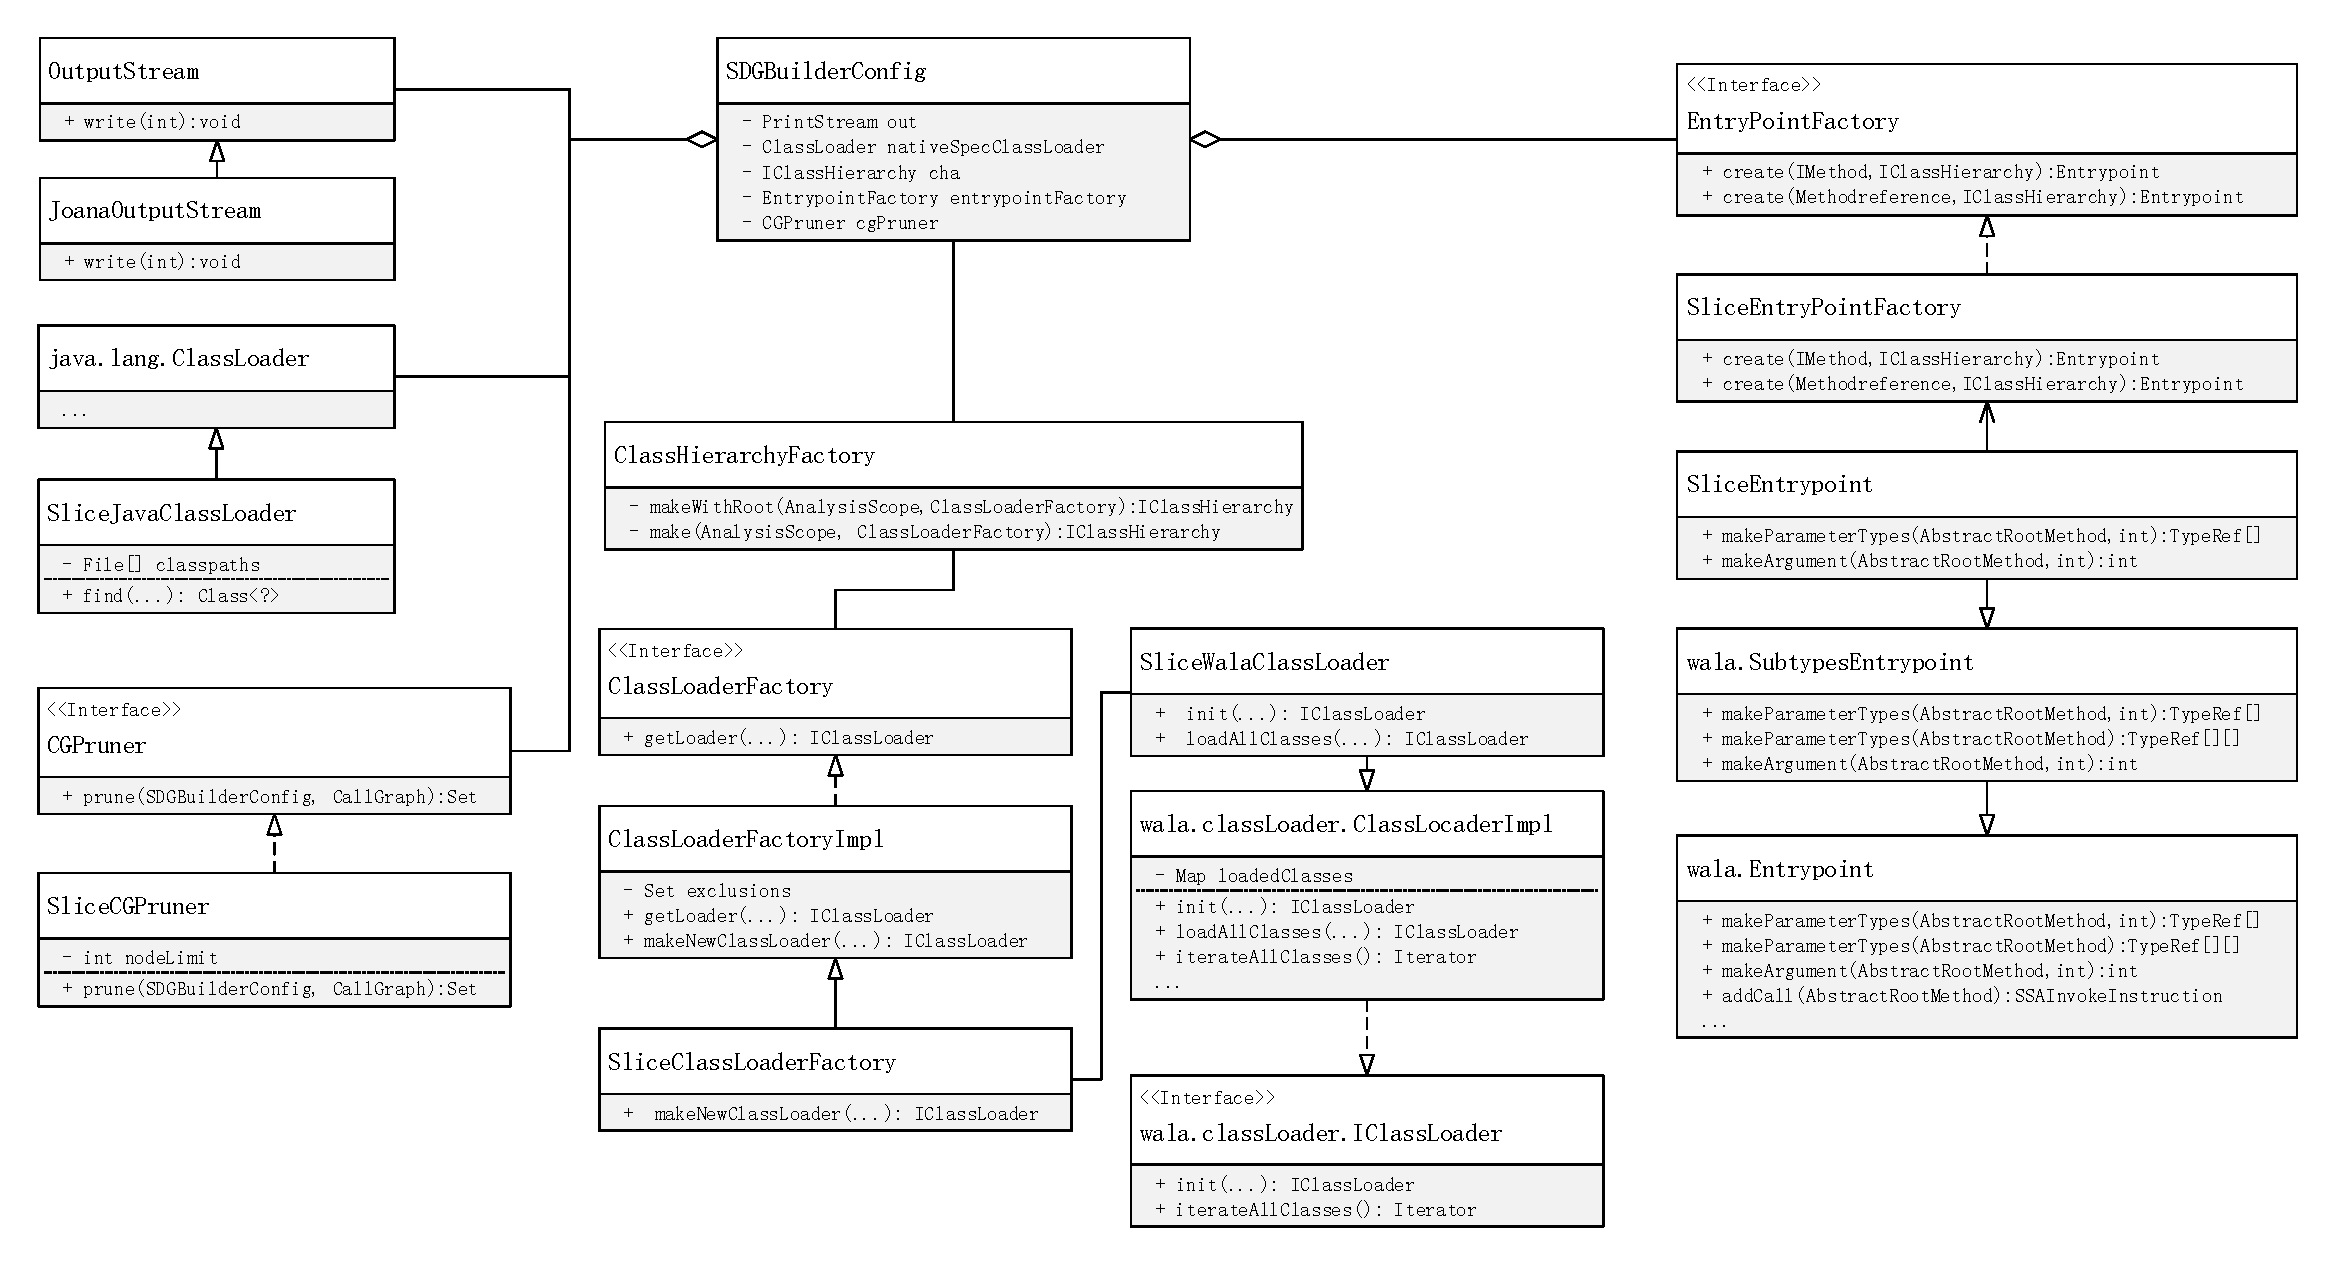
\includegraphics[width=0.9\textwidth]{FIGs/chapter4/sliceConfigClass.pdf}
    \caption{生成 SDG 的配置类图}\label{JoanaConfig}
\end{figure}

为 Joana 打印日志,构造 JoanaOutputStream 类,其继承 Java 原生的 OutputStream,其 \textit{write()} 函数用来向控制台打印日志信息,其实例作为配置的 out 属性。

SliceJavaClassLoader,SliceClassLoaderFactory 和 SliceWalaClassLoader 用于解决异形 Jar 包找不到类的问题,例如,Springboot 的项目 Jar 包中,类文件的地址前缀为 “$BOOT-INF/classes/\langle package \rangle.\langle class \rangle.class $”,首先,解决类查找问题,因为对于 Joana 切片来说,其首先通过 ClassHierarchyFactory 获取类层次图(IClassHierarchy),该图中包含了切片器能够分析的所有类,构造类的层次图首先需要遍历应用包中所有的类,其函数 makeWithRoot() 和 make() 都是构建调用图的函数,可以看到它们的第一个参数是分析范围,该对象可以通过传入的 jar 包路径创建,而第二个参数就是对 jar 包的类加载器工厂类(ClassLoaderFactory),注意这里的类加载器不等同于 Java 原生的 Classloader。类加载器为一接口(IClassLoader),其用于遍历分析范围类的所有类(\textit{iterateAllClasses()} 方法),为了解决类查找问题,首先需要在遍历时获取这些Jar包的正确类名,即重写 ClassLoader 并建立对应的工厂类。Joana 默认的(准确的说是Joana借助WALA的)类加载器为 ClassLoaderImpl,其 init() 方法通过 \textit{loadAllClasses()} 将 Jar 中的所有类读取至缓存,当调用iterateAllClasses() 时,只需遍历缓存中的类即可,因此本模块的 SliceWalaClassLoader 继承了 ClassLoaderImpl 并重写了 \textit{loadAllClasses()} 方法,其实现如代码~\ref{code:sliceWalaClassLoader} 所示,可以看到代码第 9-10 行,当包名中存在“/classes/”目录时,去除“/classes/”及前部分字符,只留下包名和类名。

\begin{minipage}[!htbp]{0.9\textwidth}
    \lstinputlisting[language=Java, caption={SliceWalaClassLoader 代码实现}, label={code:sliceWalaClassLoader}]{FIGs/chapter4/sliceWalaClassLoader.java}
\end{minipage}

接着模块需要解决类真实加载的问题,模块通过自定义Java原生ClassLoader(SliceJavaClassLoader)解决该问题,该类实现代码如代码~\ref{code:sliceJavaClassLoader} 所示,其关键在于代码第 9 行,即通过字符串尾部匹配来判断 classpath 下是否包含文件,如果包含则读取该类的内容至比特数组 classByte 中。 

\begin{minipage}[!htbp]{0.9\textwidth}
    \lstinputlisting[language=Java, caption={自定义JavaClassLoader}, label={code:sliceJavaClassLoader}]{FIGs/chapter4/sliceJavaClassLoader.java}
\end{minipage}

最后,将 ClassHierarchyFactory 产生的类层次图配置在 SDGBuilderConfig 实例的 cha 属性中。

很多用户提交的Jar包并不包含第三方包依赖信息,默认 Joana 无法完成切片,其关键问题在于以下两点:
\begin{enumerate}
    \item 当类继承于其他第三方包中类时,Joana 由于无法找到第三方类而无法构造该类。
    \item 当函数参数类型为第三方包中类时,Joana 由于无法找到类原型无法分析。
\end{enumerate}

对于第一点,模块重新编译了 Joana 使其依赖于高版本的 WALA,在生成类层次图是,使用 \textit{makeWithRoot()} 方法生成,即当该类的父类为搜索范围之外的类时,将其继承自Object类(在 Java 中 Object 类是所有类的父类)。
对于第二点,为此模块在 SliceEntrypoint 类中重新写了 Entrypoint 类的\textit{ makeParameterTypes()} 和 \textit{makeArgument()} 方法,\textit{ makeParameterTypes()} 用在函数调用语句发生时,返回函数调用参数类型,这里当调用的参数类型为范围外的类时,函数返回一个伪造的类型,\textit{ makeArgument()} 用于当函数调用发生时,为实参创建一个实例,并返回实例节点的序号,这里当实参类型为范围外的类时,伪造一个虚节点加入序号表中,并将其返回。
此外,模块实现 SliceEntrypoint 类的工厂类 SliceEntryPointFactory,并将其配置在 SDGBuilderConfig 实例的 entrypointFactory 属性中。

% TODO 解释函数调用图结构

用户上传的实际程序规模不可控,对其进行完整切片很可能造成物理资源耗尽或是程序崩溃,为此,模块在 \textit{NodeLimitPruner.prune()} 中实现了对调用图剪枝已完成限制调用图的切片,代码\ref{code:slicePruner} 描述了其过程。首先,初始化需要保留的CGNode集合 keep,接着通过广度优先搜索,向 keep 中加入不超过 nodeLimit 数量的节点,最后返回 keep 即可。

\begin{minipage}[!htbp]{0.9\textwidth}
    \lstinputlisting[language=Java, caption={NodeLimitPruner 的实现}, label={code:slicePruner}]{FIGs/chapter4/slicePruner.java}
\end{minipage}

\section{数据处理模块的实现}

数据处理模块将程序切片进行泛化和向量化处理,以保证神经网络的泛化性能,本节就泛化处理和向量化两方面说明该模块的实现。\\

\subsection{泛化处理}

在设计阶段,本文已经介绍了模块对程序切片的泛化主要分泛化数字常量、泛化字符串常量、泛化变量、泛化函数调用和泛化包名方法名五个方面,下面以 \textit{unsafe()} 函数的代码切片~\ref{code:sliceDemo}为例,介绍这些泛化的具体含义。

\begin{minipage}[!htbp]{0.9\textwidth}
    \lstinputlisting[language=Java, caption={\textit{unsafe()} 函数的代码切片}, label={code:sliceDemo}]{FIGs/chapter4/sliceDemo.txt}
\end{minipage}

首先是泛化数字常量,数字常量在切片中往往带有数据信息,然而程序切片中的数字返回往往变化很大,为了泛化总结出共性,模块将三位数及以上的整数同一替换为“N3P”,将三位数及以上的负整数替换为“NN3P”,将科学计数法的数字替换为“NSMALL”,剩余三位数一下数字将其“\#()”去除保留数字字符串,如在示例切片第 3 行中的“\#(0)”,将其替换为 “0”。

字符串常量在切片代码中非常常见,其内容也很可能是判断一个切片是否是安全的重要标准,如 SSRF 漏洞切片中发现有 “http”开头的字符串,那么漏洞很可能是误报,或是注入型漏洞出现特殊符号的替换字符串,那么这些漏洞也很可能是误报。因此,对于字符串要做特殊泛化处理,首先,若包含如“HTTP”,“HTTPS”且长度大于其4的字符串,将其泛化为“URL”;此外,若字符串长度大于 2,因为这些字符串是清洁字符串的概率较小,将其泛化为“STR S\{i\}”的形式,i 指该字符串为切片中出现的第 i 个字符串;否则保留其本身,因为其本身很可能是清洁类字符串。例如在第 2 行切片中出现的“\#(clean)”,则将其泛化为 “STR S1”(其为切片中出现的第一字符串)。

由于切片对象为静态单赋值形式(SSA),以“v\{数字\}”的变量在切片中很常见,但是由于切片原因,这些数字并不是自然增长的,因此在泛化流程中,对其出现顺序进行映射,将其泛化为“VAR V\{i\}”的形式,其中 i 代表该变量是第 i 个出现在切片中的,例如第 2 行、第 3 行和第 4 行出现的 v6 变量,将其泛化为“VAR V1”,即该变量第 1 个出现在切片中。

泛化函数调用主要是针对于调用切片和返回,对于调用切片,如第 2 行,将其调用函数前的“.”去除,若有形参(“\$”开头的变量)也将其去除,因为形参名称与漏洞本身无关,并在括号前后加空格,当做完经过该步骤后,第 2 行切片的函数调用部分泛化为“VAR V1 = p1 equals ( STR S1 ) ”,若函数调用返回为对象,则将其下划线形式改为“.”连接的形式,如最后一行中的“Ljava/lang/String”变为“java.lang.String”。

泛化包名方法名,此类泛化主要对于 ENTER 类型的节点,如第 1 行,这里需要将切片才分为“包名\_方法名\_函数参数类型”,如将“demo.XSS.unsafe(java.la-\\ng.String)”泛化为“demo XSS unsafe ( java.lang.String )”。\\

\subsection{建立单词表与向量化}

在本模块中,泛化后字符串首先生成单词表,再按照单词表可以对句子进行向量化。其实现代码如代码~\ref{code:preTokenize} 所示。

\begin{minipage}[!htbp]{0.9\textwidth}
    \lstinputlisting[language=Python, caption={建立单词表和向量化的实现}, label={code:preTokenize}]{FIGs/chapter4/preTokenize.py}
\end{minipage}

\textit{build\_Dict()} 方法输入为切片数据集,方法首先建立一个空的字典和词频表,接着遍历数据集中的所有切片,按空格拆分,并开始统计词频,遍历结束后,根据词频表,将词频大于 freq\_gt 的单词放入单词表,单词进入单词表的顺序将成为其id,小于等于该词频的单词会被映射为“UNK”,方法最终返回一个单词字典。
\text{encode()} 方法用于将一个切片数据向量化,其只需要将切片拆分为单词,再通过字典将每一个单词映射为 id 即可,方法最终返回为一个句子的向量。\\

\section{误报预测模块的实现}

\subsection{误报预测控制}
误报预测控制负责执行图~\ref{predictProcessing} 中的主要流程,其代码如~\ref{code:predictRunner} 所示。

\begin{minipage}[!htbp]{0.9\textwidth}
    \lstinputlisting[language=Java, caption={误报预测控制逻辑的实现}, label={code:predictRunner}]{FIGs/chapter4/predictRunner.java}
\end{minipage}

代码遍历 sliceProject 中的每一个实例、每个实例中的每个污点传播树,以及每个传播树中的污点传播流,从代码 20-23 行可以看出,只要树中的一条传播流是安全的,那么整个传播树就是安全的,对应的安全流会保存到 safeFlows 集合中。从第 27 行可以看到,只有当所有的污点传播树都是安全时,一个漏洞实例才可判断为误报,最后,将安全的流放入预测项目中作为证明,以及将是否为误报的结果也放入项目中。\textit{flowIsSafe()} 在调用远程预测服务前,会先检查缓存是否已有记录,若存在记录则直接将其返回,否则调用远程服务。\\

\vspace{1cm}
\subsection{误报预测时序图}
误报预测模块存在客户端至服务器调用流程,本文通过时序图~\ref{predictTime} 说明误报预测的调用实现。

\begin{figure}[!htb]
    \centering
    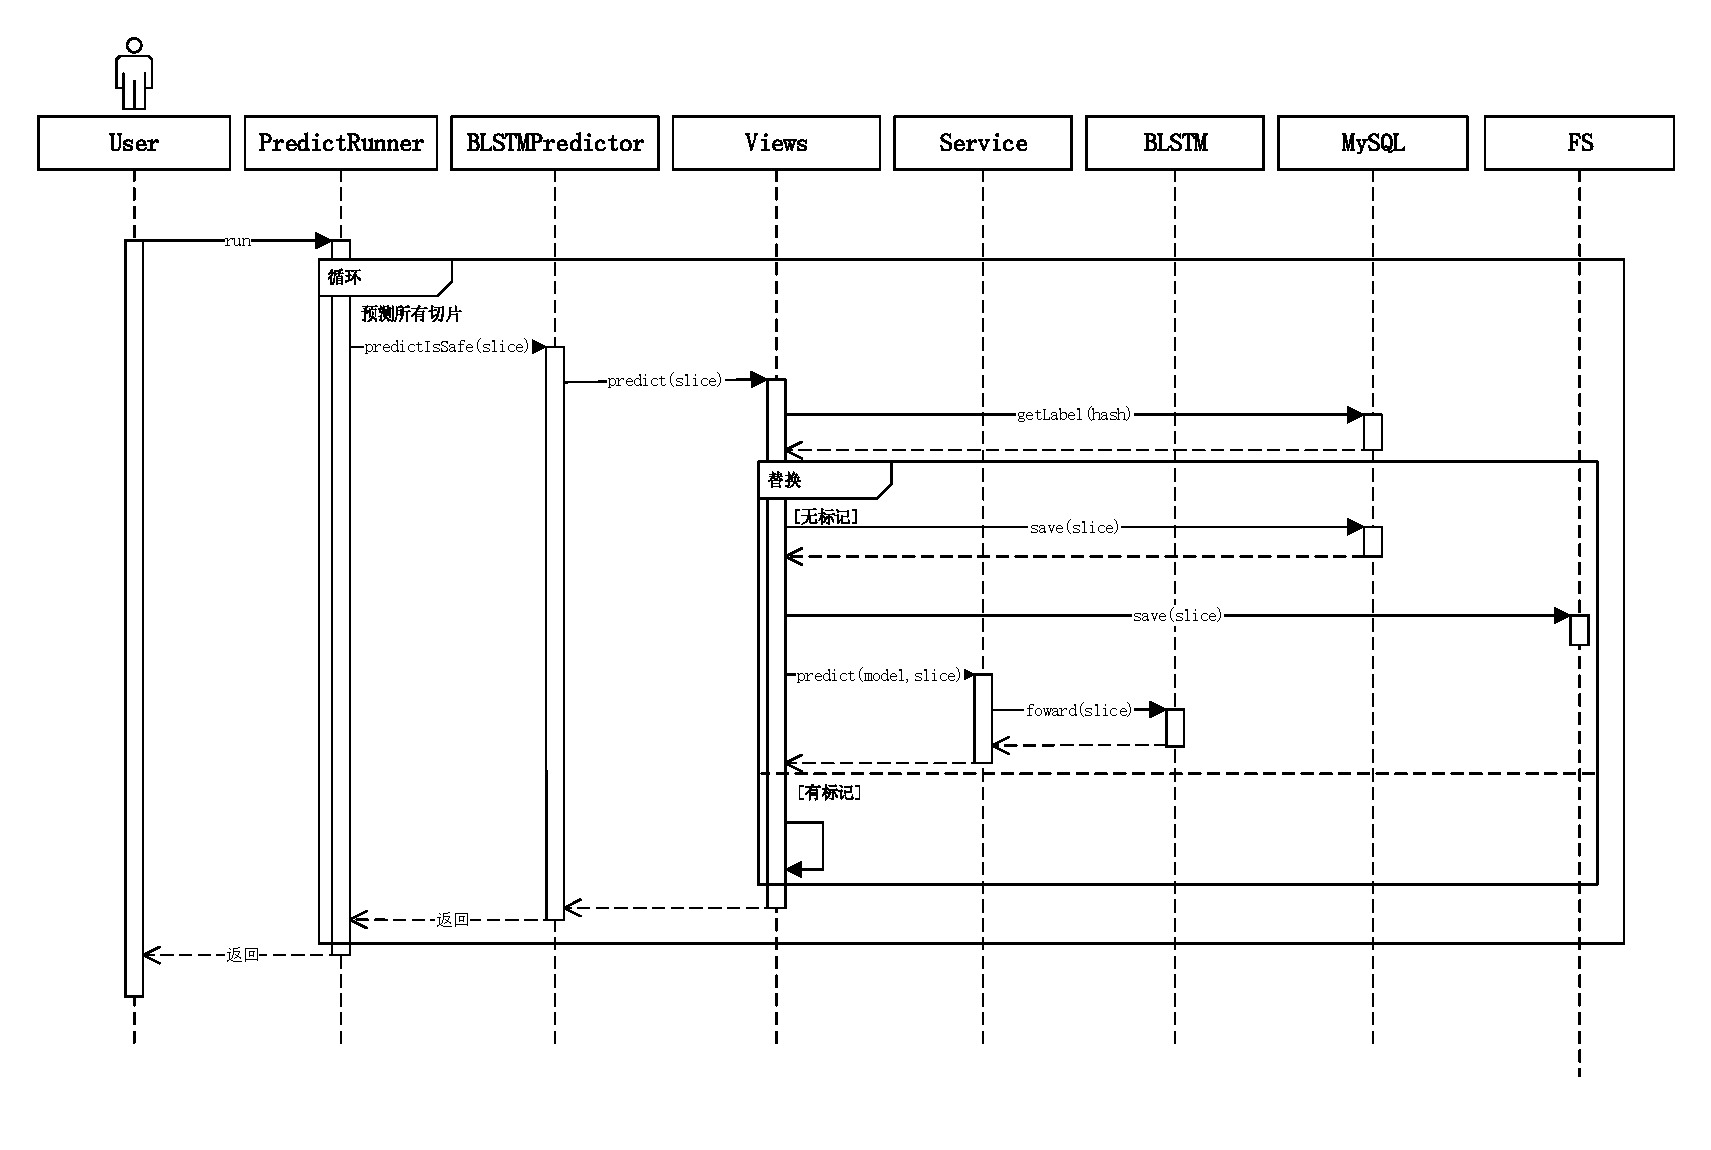
\includegraphics[width=0.9\textwidth]{FIGs/chapter4/predictTime.pdf}
        \vspace{-1cm}
    \caption{误报预测时序图}\label{predictTime}
\end{figure}

用户首先发起对污点传播报告的预测请求,接着预测控制逻辑进入循环,对于每一个切片调用 BLSTMPredictor 进行预测,BLSTMPredict 远程服务的本地代理,其会向远程服务器发送预测请求,服务器视图层收到预测请求后,首先从数据库查找该切片是否有标记,如果有标记则优先返回标记数据,否则先将切片一次保存至数据库和本地文件系统中,再向预测服务发起预测请求,预测服务收到请求后发送给 BLSTM 模型,模型将预测结果依次返回至用户。\\

\vspace{2cm}
\subsection{漏洞标记时序图}

本模块的另一重要流程在于对漏洞实例的标记,时序图~\ref{labelTime} 展示了漏洞标记的实现过程。

\begin{figure}[!htb]
    \centering
    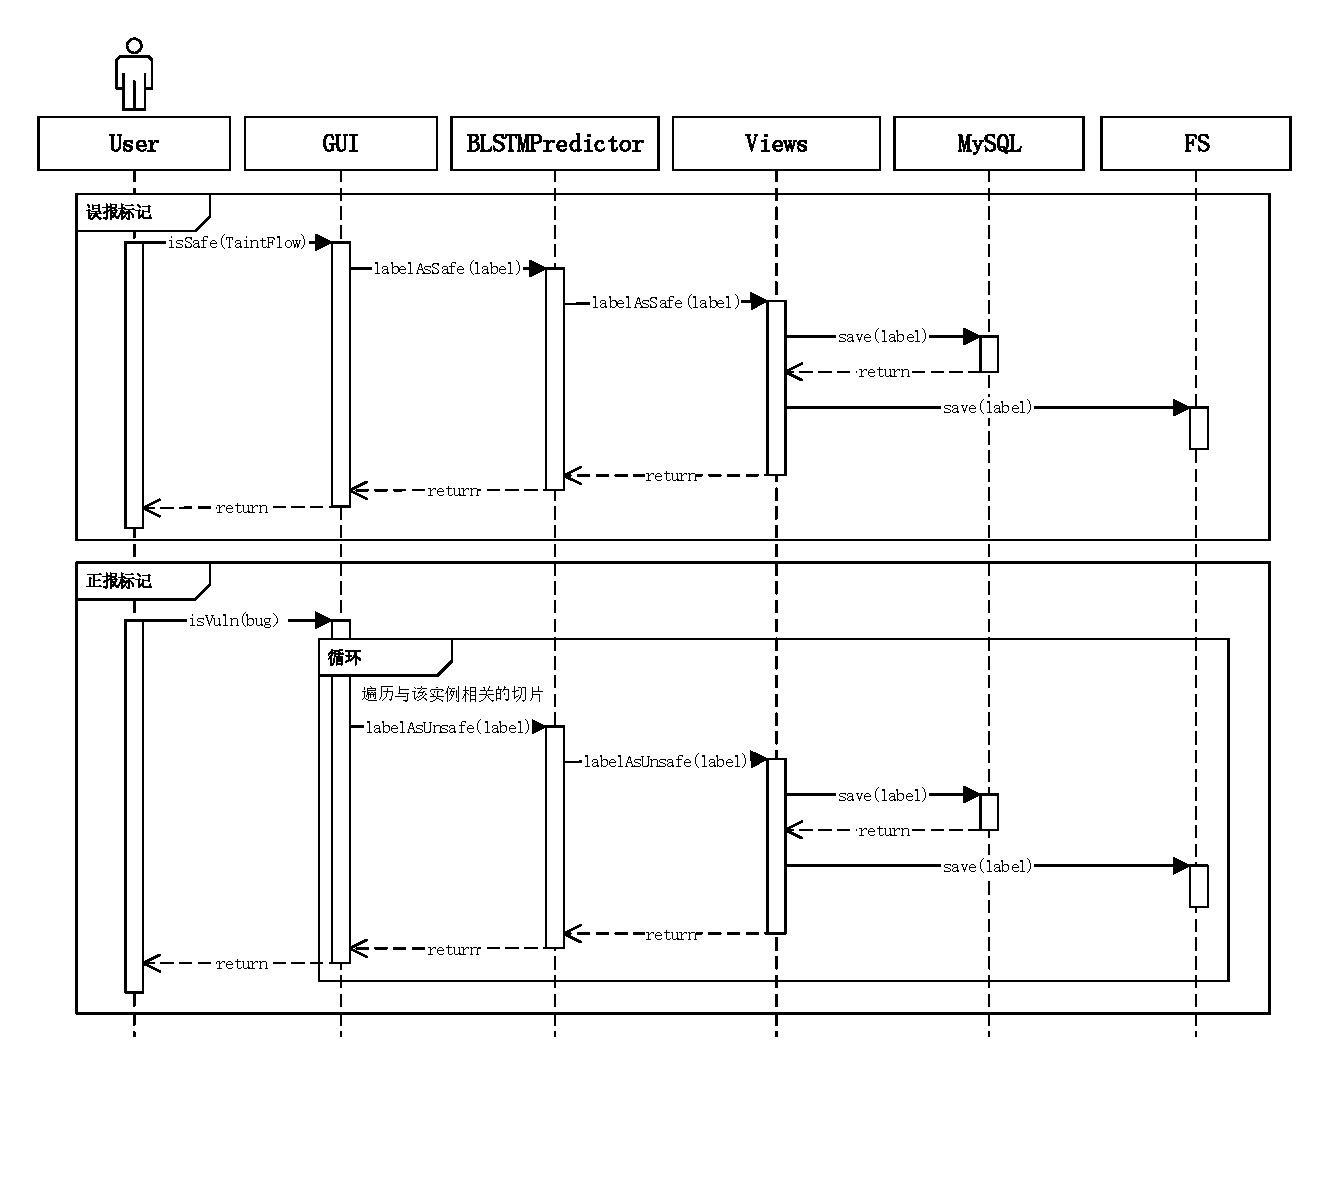
\includegraphics[width=0.9\textwidth]{FIGs/chapter4/labelTime.pdf}
    \vspace{-1cm}
    \caption{漏洞标记时序图}\label{labelTime}
\end{figure}

用户可以对一个漏洞进行误报或正报的标记,首先看误报标记流程,对于一个误报漏洞实例,用户首先需要提供证据,即指定污点消失于哪一段污染流中,接着GUI界面会生成一个 Label 实例并向预测器发送标记为安全污染流的请求,本地预测器会将请求转发到服务端的 View 层,View 层收到请求后将标记数据依次写入数据库和本地文件中,由于污染流哈希的唯一性,当数据库存在已有标签时会自动覆盖。

对于一个正报标记,用户只需指定漏洞实例的一个传播树即可,因为一个真实的漏洞的只要有一棵传播树的污点传播成立,该漏洞就是真实存在的,因此 GUI 收到请求后会遍历传播树相关的所有切片,并发送标记为不安全的标签。对于每一个不安全标签的标记时序与安全标记时序相同,这里不再赘述。

\subsection{批处理训练过程}

用户在 Web 端可以发起训练任务,Celery Worker 收到训练任务后,会调用训练服务按指定配置训练 BLSTM 神经网络。

% https://www.zhihu.com/question/32673260
该模型训练时的输入为切片向量集合,对应标记集合,输出为一个训练好参数的 BLSTM 模型。由于程序切片大小有差异,切片向量长度也是不一致的,对于时序型神经网络 BLSTM 来说,本身就具有接受不定长向量的能力,然而在实际训练时,为了保证训练效率和效果,往往会将一批切片向量和对应标记合并一为一批输入神经网络,再进行权重更新,这时一组切片向量需要转换为二维向量,即需要对末尾补 0,因此在BLSTM模型中,要考虑到补 0 的无效数据。

Pytorch 的 DataLoader 对象运行设定一个校对函数 \textit{collate\_fn()},该函数用于从数据集加载数据后,对数据进行最后处理,本模块根据需要构造的校对函数如代码~\ref{code:collateFn} 所示。

\begin{minipage}[!htbp]{0.9\textwidth}
    \lstinputlisting[language=Python, caption={DataLoader 的加载器}, label={code:collateFn}]{FIGs/chapter4/collateFn.py}
\end{minipage}

可以看出,该函数的输入为一个向量化类和一批数据集合,该集合中存放切片字符串和对应标记对,对于每一个标记对,首先调用预处理模块对其泛化和向量化(第 3 行),接着按切片长度从长到短对一批数据排序,获取每条切片的长度记为 data\_length 变量,使用 pytorch 预定义的函数 \textit{rnn\_utils.pad\_sequence()} 对已排好序的一批数据进行补 0,此时 data\_x 类型已由原先的 list 类型变为二维张量(Tensor)类型,最后将这批数据的标记作为一维向量,最后函数返回切片张量(二维),切片长度张量(一维)和标记(一维)。

接着切片张量和切片长度张量将传递至 BLSTM 类的 forward() 方法中,代码~\ref{code:blstm} 展示了神经网络后向传播的细节。

\begin{minipage}[!htbp]{0.9\textwidth}
    \lstinputlisting[language=Python, caption={DataLoader 的加载器}, label={code:blstm}]{FIGs/chapter4/blstm.py}
\end{minipage}

首先,对于切片张量进行词嵌入,其输出的 embeds 即变为三维张量,注意这里词嵌入已经指定了 padding 值,即将补其用的数字映射为全 0 向量。接着使用 pytorch 定义的 \textit{rnn\_utils.pack\_padded\_sequence()} 函数将实际上不等长的切片向量打包,接着打包数据传递至 BLSTM 层,再将 BLSTM 层输出还原至三维张量,注意,此时张量规模为记录数 $\times$ 最长语句长度 $\times$ BLSTM神经元个数。 \textit{get\_last\_output()} 会获取该三维张量上每一记录的双向传播时最后一时刻的神经元输出,并整合为一二维张量,最终输出到线性层,线性层返回预测结果。

\begin{figure}[!htb]
    \centering
    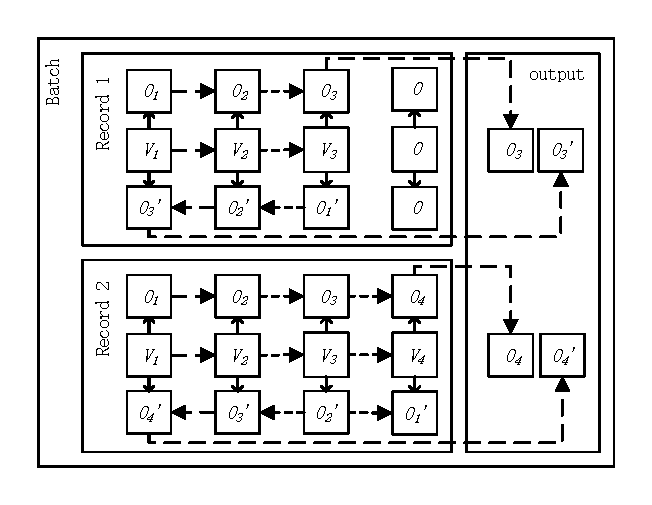
\includegraphics[width=0.9\textwidth]{FIGs/chapter4/blstmFoward.pdf}
    \caption{批处理训练示意图}\label{blstmForward}
\end{figure}

图~\ref{blstmForward} 展示了 \textit{get\_last\_output()} 的具体做法,假设一批数据中存在两条数据 record 1 和 record 2, 它们有效的切片向量长度为 3 和 4,经过 BLSTM 神经网络后,正反方向分别产生了每个时刻上的输出,此时对于记录 1 来说,需要提取最后一个时刻的神经元输出,即 $O_3$ 向量和 $O_3'$ 向量,并将其合并,对于记录 2 来说,提取并合并为 $\left[O_{4}, O_{4}'\right]$,最后该批数据为二维张量,再输入至线性层,也就是说,线性层神经元个数为 BLSTM 神经元个数的两倍。

\section{系统测试与运行展示}
\subsection{测试目标}
本系统测试主要安排功能测试和性能测试,在功能测试方面主要对系统功能的正确性进行测试;而健壮性和性能测试主要关注于本系统在扫描各类被测应用时的程序不崩溃,并能在合理时间内返回数据。

在功能测试中,主要对第~\ref{sec:demand} 节提出的需求和用例进行测试,对污点分析、程序切片、预处理和误报预测各个模块的生成测试用例并对其进行测试。在健壮性测试中,主要对系统输入各类 Jar 包,检查系统是否能否在规定时间内产生扫描报告。

表~\ref{tab:testenv}为测试的软硬件环境,在硬件方面,由于扫描任务是计算密集型任务,所以客户端选择了 CPU 较高配置的 E5-2630 和内存为 32G,并将 JVM 参数调整为“-Xmx8g -Xss500m”,服务端的硬件配置与客户端相同,软件上有Pytorch、Django、Celery、MySQL和Redis。

\begin{table}[!htbp]\footnotesize
    \centering
    \caption{系统测试软硬件环境}
    \begin{tabular}{cll}
        \toprule
        \multicolumn{2}{c}{设备与软件} & 备注信息 \\
        \midrule
        \multirow{3}[2]{*}{客户端} & CPU   & 型号为 Intel(R) Xeon(R) CPU E5-2630 v3 @ 2.40GHz \\
        & 内存    & 大小为 32G \\
        & Java  & JVM 参数为“-Xmx8g -Xss500m ”\\
        \midrule
        \multirow{7}[2]{*}{服务端} 
        & CPU   & 型号为 Intel(R) Xeon(R) CPU E5-2630 v3 @ 2.40GHz \\
        & 内存    & 大小为 32G \\
        & Pytorch & 版本为 1.3.1 \\
        & Django & 版本为 2.2.5 \\
        & Celery & 版本为 4.4.0 \\
        & MySQL & 版本为 8.0.12 \\
        & Redis & 版本为 3.0 \\
        \bottomrule
    \end{tabular}%
    \label{tab:testenv}%
\end{table}%

\subsection{功能测试}
本章节主要针对各个模块的主要功能设计测试套件,并对每个测试套件进行具体测试。测试套件如表~\ref{testsuitcase} 所示。

\begin{table}[!htb]\footnotesize %label table
    \centering
    \caption{系统测试用例套件}
    % l - left, r - right, c - center. | means one vertical line 这里声明的是表格单元中的内容如何对齐
    \begin{tabular}{L{0.5cm}L{2cm}L{3cm}L{7cm}}
        \toprule
        \textbf{ID} & \textbf{所在模块} &\textbf{测试功能} &\textbf{测试内容}\\
        \midrule
        TS1 & 污点分析模块 & 基于污点分析的静态扫描  & 提交扫描任务,系统能够将污点分析结果显示在用户界面。\\
        TS2 & 污点分析模块  & 污点分析结果的存取 & 对于一个污点分析结果,系统可以将其保存,并在打开时导入。\\
        TS3 & 程序切片模块  & 程序切片 & 对于一个污点分析项目,对每一个漏洞进行切片,生成程序切片项目\\
        TS4 & 预处理模块   & 切片泛化与向量化 & 对于一个切片文本,对其进行泛化和向量化\\
        TS5 & 误报预测模块  & 预测漏洞安全性 & 对于一个漏洞实例,利用模型预测其是否为误报\\
        TS6 & 误报预测模块  & 标记漏洞安全性 & 对于一个漏洞实例,标记该漏洞是否为误报\\
        TS7 & 误报预测模块  & 模型训练 & 指定模型训练配置,根据配置训练模型\\
        \bottomrule
    \end{tabular}
    \label{testsuitcase}
\end{table}

在污点分析模块,主要有测试套件 TS1,对用户提交的 Jar 包集合进行污点分析,并将污点分析结果以漏洞实例和对应若干棵污点传播树的形式返回给用户;测试套件 TS2,用户对于污点分析结果,进行存取操作。其包含的测试用例如表~\ref{testcase:taint} 所示,TS1 中含一个测试用例 TC1-1;TS2 套件中含两个测试用例,TC2-1 和 TC2-2, 分别测试对于结果的保存和读取。经过测试,得出的测试结果与预期结果相符,测试用例全部通过。

\begin{table}[!htbp]\footnotesize
    \centering
    \caption{基于污点分析的静态扫描测试用例}
    % l - left, r - right, c - center. | means one vertical line 这里声明的是表格单元中的内容如何对齐
    \begin{tabular}{L{0.07\textwidth}L{0.2\textwidth}L{0.18\textwidth}L{0.3\textwidth}L{0.09\textwidth}} 
        \toprule
        \textbf{ID}&\textbf{说明} & \textbf{输入}&\textbf{预期输出}&\textbf{测试结果}\\
        \midrule
        TC1-1 & 污点分析 & 用户提交的 Jar 包  & 污点分析结果(显示到界面) & 通过 \\
        TC2-1 & 污点分析结果保存 & 污点分析结果  & 记录分析结果的XML文件 & 通过 \\
        TC2-2 & 污点分析结果读取 & 记录分析结果的XML文件  &  污点分析结果 & 通过 \\
        \bottomrule
    \end{tabular}
    \label{testcase:taint}
\end{table}

在程序切片模块,主要有一个测试套件TS3,即测试系统能否成功将污点分析项目转化为切片项目,在切片项目中,存在污点传播树和其对应的污点传播流,每个污点传播对应一条切片。该测试套件对应的测试用例如表~\ref{testcase:slice} 所示,其主要包含有 TC3-1,对上一模块产生的分析结果进行处理,从报告中还原污点传播树;TC3-2,拆解污点污点传播树,将一颗传播树拆解为子污染流的集合;TC3-3,对一个污染流进行后向切片,由于 Joana 自身存在 bug,当切片成功时,程序返回切片文本,在切片失败时扫描任务不崩溃,并返回错误原因。经过测试,以上测试用例输出均与预期相符,测试全部通过。

\begin{table}[!htb]\footnotesize
    \centering
    \caption{程序切片测试用例}
    % l - left, r - right, c - center. | means one vertical line 这里声明的是表格单元中的内容如何对齐
    \begin{tabular}{L{0.07\textwidth}L{0.2\textwidth}L{0.18\textwidth}L{0.3\textwidth}L{0.09\textwidth}}
        \toprule
        \textbf{ID}&\textbf{说明} & \textbf{输入}&\textbf{预期输出}&\textbf{测试结果}\\
        \midrule
        TC3-1 & 处理污点分析结果  & 污点分析结果 & 漏洞实例及其对应传播树集合 & 通过\\
        TC3-2 & 拆解污点传播树  & 污点传播树 & 子污染流集合 & 通过\\
        TC3-3 & 污染流后向切片  & 污染流 & 切片文本(若失败返回错误原因) & 通过\\
        \bottomrule
    \end{tabular}
    \label{testcase:slice}
\end{table}

数据预处理模块的测试套件为 TS4,其用于测试改模快是否能对于一个切片文本进行泛化和向量化处理。其包含的测试用例如表~\ref{testcase:preprocessing} 所示,TC4-1 用于测试预处理模块能否对于一个切片文本进行有效泛化处理,对其输出单词序列;TC4-2 用于测试模块对于单词序列集合,能否将其转化为向量集合和对应的单词表,在输入时,单词表为可选项,若不存在单词表则新建,存在则根据已有单词表进行向量生成。经过测试,以上测试用例输出均与预期相符,测试全部通过。

\begin{table}[!htb]\footnotesize
    \centering
    \caption{数据预处理模块测试用例}
    % l - left, r - right, c - center. | means one vertical line 这里声明的是表格单元中的内容如何对齐
    \begin{tabular}{L{0.07\textwidth}L{0.2\textwidth}L{0.18\textwidth}L{0.3\textwidth}L{0.09\textwidth}}
        \toprule
        \textbf{ID}&\textbf{说明} & \textbf{输入}&\textbf{预期输出}&\textbf{测试结果}\\
        \midrule
        TC4-1 & 泛化处理  & 切片文本 & 单词序列 & 通过\\
        TC4-2 & 向量化处理  & 单词序列集合和单词表(可选) & 单词对照表和向量集合 & 通过\\
        \bottomrule
    \end{tabular}
    \label{testcase:preprocessing}
\end{table}

误报预测模块的测试套件有 TS5,对漏洞实例安全性进行预测;TS6,对漏洞实例安全性进行标记;TS7,对已有新数据进行模型训练。它们对应的测试用例如表~\ref{testcase:predict} 所示,安全性实例预测套件对应的测试用例有 TC5-1,对切片文本进行安全性预测,由于切片文本与污染流成一一对应关系,切片文本安全即污染流安全,测试检查系统是否能返回预测结果,并同时将污染流保存到文件系统和数据库中;TC5-2,对一个漏洞实例进行误报预测,测试给定任意漏洞实例和对应传播树的集合,系统能否返回漏洞是否为误报。安全性标记对应的测试用例有 TC6-1,标记污染流安全性,对于单个污染流标记其是否安全,系统需要将该标记数据存储至数据库和文件系统中,更新预测结果;TC6-2,标记可利用的传播树,系统需要将其对应的所有污染流标记为不安全,其对应的漏洞也应标记为不安全。模型训练对应的测试用例有 TC7-1,用户在后台新建训练配置,系统将其配置保存至数据库;TC7-2,用户发起训练请求,系统异步完成请求,并将训练好的模型保存至数据库和文件系统。经过测试,以上测试用例输出均与预期相符,测试全部通过。 

\begin{table}[!htb]\footnotesize
    \centering
    \caption{误报预测模块测试用例}
    % l - left, r - right, c - center. | means one vertical line 这里声明的是表格单元中的内容如何对齐
    \begin{tabular}{L{0.07\textwidth}L{0.2\textwidth}L{0.18\textwidth}L{0.3\textwidth}L{0.09\textwidth}}
        \toprule
        \textbf{ID}&\textbf{说明} & \textbf{输入}&\textbf{预期输出}&\textbf{测试结果}\\
        \midrule
        TC5-1 & 切片文本安全性预测 & 污染流和对应切片 & 预测结果,同时污染流保存到文件系统和数据库 & 通过\\
        TC5-2 & 漏洞误报预测  & 漏洞实例和对应传播树集合 & 漏洞是否为误报 & 通过\\
        TC6-1 & 标记污染流  & 污染流切片和标记 & 更新预测结果,标记存储至数据库和文件系统中 & 通过\\
        TC6-2 & 标记可利用的传播树  & 污点传播树 & 更新预测结果,所有对应的污染流标记为不安全并存储至数据库和文件系统 & 通过\\
        TC7-1 & 新建训练配置 & 训练配置 & 生成配置存储至数据库 & 通过\\
        TC7-2 & 发布训练任务 & 训练任务请求 & 异步进行任务训练,并将训练完成的数据保存到数据库和文件系统 & 通过\\
        \bottomrule
    \end{tabular}
    \label{testcase:predict}
\end{table}

\subsection{健壮性和性能测试}

为了测试本系统的健壮性和性能,本文选择 Maven 中央仓库流行度 Top 100 的项目,在每个项目选择使用最多的构建版本作为测试对象~\footnote{\url{https://mvnrepository.com/popular?p=1},抓取时间为 2019年10月24日,当前流行度榜单可能已经发生变化} 批量建立扫描任务进行测试,表~\ref{robustTest} 列出了测试结果,对于一个项目,本文将系统的最大扫描时间设为 4 小时,如果超过该时间系统仍未返回结果,则认为系统扫描失败。

\begin{table}[!htb]\footnotesize
    \centering
    \caption{健壮性和性能测试结果}
    % l - left, r - right, c - center. | means one vertical line 这里声明的是表格单元中的内容如何对齐
    \begin{tabular}{llllll}
        \toprule
        \textbf{测试 Jar 包}&\textbf{合法 Jar 包} & \textbf{扫描成功率} &\textbf{最短扫描时间(s)}&\textbf{平均扫描时间(s)} & \textbf{最长扫描时间(s)} \\
        \midrule
        96 & 82 & 100\%  & 7.21 & 67.22 &1815.24 \\
        \bottomrule
    \end{tabular}
    \label{robustTest}
\end{table}

其中有 4 个构建为 aar 格式,由于系统只能输入 Jar 格式,因此实际参与测试的文件为 96 个 Jar 包文件,在 96 个 Jar 文件中,有 14 个Jar 文件内无 “.class”文件,系统均在能启动扫描时检测并提示用户 Jar 包不合法,并正常退出。对于剩下的 82 个文件,系统在限定时间内返回扫描结果,即扫描成功率为 100\%,至此本文认为该系统具有较高的健壮性。

在系统性能方面,可以看出对于测试的 Jar 包,系统最短扫描时间仅有 7.21 s,对应的 Jar 包为 support-annotations-27.1.1.jar~\footnote{\url{https://mvnrepository.com/artifact/com.android.support/support-annotations/27.1.1}},这一类包的特点在于其本身项目较小,项目中与安全有关的函数(Sink 点)调用也相对较少,因此其分析时间也较短;平均扫描时间为 67.22s,这也意味着对于绝大多数的 Jar 包,开发者在一分钟左右即可收到扫描结果;系统最长扫描时间为 1815.24s,对应的 Jar 包为 groovy-all-2.4.7.jar ~\footnote{\url{https://mvnrepository.com/artifact/org.codehaus.groovy/groovy-all/2.4.7}},该包为 Groovy 语言的解释器,因此代码中会出现大量的安全相关函数和入口点,因此分析时间较长,但是系统仍能在一个小时之内给出扫描报告,对于大型项目而言,本文认为这是合理的。

本系统对于各类 Jar 包有较高的健壮性,并且能较为及时的完成扫描任务,在保证代码安全同时不会影响代码开发进度。\\

\subsection{系统效果评估}

\subsubsection{研究性问题}
相对于传统污点分析系统,本系统主要采取神经网络预测降低污点分析报告误报来提升准确性,在本小节,将从两个研究性问题入手,证明本系统相较于传统安全分析工具的优势:

\begin{itemize}
    \itemindent 2.8em
    \item[\textbf{RQ1:}] 与目前流行的污点分析系统相比,本系统是否能有效降低误报?
    \item[\textbf{RQ2:}] 对于本系统中预测的基本单位——污点传播流,本系统模型是否有较高的准确性?
\end{itemize}

\textbf{RQ1} 直接回答了用户最关键的问题,因为本系统的主要目标即降低误报提高准确性。
\textbf{RQ2} 更进一步的解释了系统能够取得较高提升的原因,因为系统的预测模型实际是对污染流对应的切片进行切片,其污染流的预测准确性直接影响了误报预测的准确性。\\

\subsubsection{参数设置}
本系统的 BLSTM 预测模型在训练和构造时存在一系列参数,系统上线前本文对已有数据集进行了测试,在权衡准确性和效率后,系统选择的参数配置如下:词嵌入维度(embedding\_dim)为 16;隐藏层神经元个数为 32;最小词频为 4;批处理记录数为32;基础学习率为 0.01;提前停止忍耐度为3;最大迭代次数为20。\\

\subsubsection{评估方法和度量}
\begin{table}[htbp]\footnotesize
    \centering
    \caption{漏洞扫描报告混淆矩阵}
    \begin{tabular}{clll}
        \toprule
        \multicolumn{2}{c}{\multirow{2}[4]{*}{}} & \multicolumn{2}{c}{扫描结果} \\
        \cmidrule{3-4}    \multicolumn{2}{c}{} & 存在漏洞  & 无漏洞 \\
        \midrule
        \multirow{2}[2]{*}{真实结果} & 存在漏洞  & TP    & FN \\
        & 无漏洞   & FP    & TN \\
        \bottomrule
    \end{tabular}%
    \label{tab:confusionMatrix}%
\end{table}

在 \textbf{RQ1} 中,本文将本系统与目前流行的 FindSecBugs 扫描报告做对比,将数据集的 90\% 作为训练集,10\% 作为测试集(对于 FindSecBugs 而言,其没有训练过程,只对测试集用例进行扫描)再根据两系统的扫描报告,以准确率(Accuracy)、精确率(Precision)、找回率(Recall)和 $F_{1}$ 作为度量比较系统准确性,为了解释这些度量计算方法,首先介绍对于扫描报告的混淆矩阵,如表~\ref{tab:confusionMatrix} 所示,对于每一个测试用例,扫描结果会对其报告为存在漏洞和不存在漏洞,因此产生实际为漏洞且扫描结果为漏洞的用例数 TP,实际为漏洞且扫描结果为无漏洞的用例数 FN (漏报数),实际无漏洞且扫描结果为有漏洞的用例数 FP(误报数)和实际无漏洞且扫描结果为无漏洞的用例数 TN,在此基础上,报告的准确率计算方式为 $Accuracy=\frac{TP+TN}{TP+FN+FP+FN}$、漏洞精确率为 $Precision=\frac{TP}{TP+FP}$、漏洞召回率为 $Recall=\frac{TP}{TP+FN}$ 以及 $F_1$ 计算方式为 $F_{1}=\frac{2 \cdot Precision \cdot Recall}{Precision+Recall}$。

在 \textbf{RQ2} 中,首先使用污点分析和切片模块得到污染流切片,再根据数据集标签对污染流进行标记,并使用预处理和预测模块对其进行训练,最后通过预测结果的混淆矩阵评估预测效果。

不论在 \textbf{RQ1} 还是 \textbf{RQ2} 中,本文每次实验重复三次取平均值作为最终结果。

\subsubsection{评估数据集}
本文使用 OWASP Benchmark v1.1~\footnote{https://owasp.org/www-project-benchmark/} ( 简称 OWASP)和 Juliet Test Suite for Java v1.3~\footnote{https://samate.nist.gov/SARD/testsuite.php} ( 简称 Juliet)作为数据集,由于 Juliet 数据集存在大量多个入口点共用一个汇聚点的漏洞情况,导致大部分漏洞均为正报(因为只要漏洞实例中任意一棵传播树是不安全的,那么漏洞就是真实存在的),从而无法在 RQ1 中使用,其将在 RQ2 和真实系统上线时,作为切片训练集使用,表~\ref{tab:dataset} 中显示了各个数据集中的数据量大小。

\begin{table}[htbp]\footnotesize
    \centering
    \caption{效果评估数据集}
    \begin{tabular}{L{0.15\textwidth}R{0.1\textwidth}R{0.1\textwidth}R{0.08\textwidth}R{0.08\textwidth}R{0.08\textwidth}R{0.08\textwidth}}
        \toprule
        & 测试用例总数 & 真实漏洞用例数 & 无漏洞用例数 & 安全污染流 & 不安全污染流 & 污染流总数 \\
        \midrule
        OWASP & 10769 & 6377  & 4392  & 3501  & 6377  & 6377 \\
        Juliet & 5217  & /     & /     & 550   & 3823  & 4373 \\
        \textbf{RQ2} 实验数据 & /     & /     & /     & 4051  & 6927  & 10978 \\
        \bottomrule
    \end{tabular}%
    \label{tab:dataset}%
\end{table}%

由于本系统只能处理部分类型,因此本文对以上两个数据集进行筛选,去掉了 FindSecBugs 中无法用污点分析检测的漏洞类型,因此表中测试用例总数会比数据集公布的数目少,对于 Juliet 数据集,由于其中不安全的数据流较多,直接用于模型训练会造成数据倾斜,因此本文只随机挑选与安全数据流数量相等的不安全数据流用于训练和测试。\\

\subsubsection{RQ1 实验结果}

\begin{table}[htbp]
    \centering
    \caption{本系统与 FindSecBugs 对比结果}
    \begin{tabular}{lrrrr}
        \toprule
        & \multicolumn{1}{l}{准确率} & \multicolumn{1}{l}{精确率} & \multicolumn{1}{l}{召回率} & \multicolumn{1}{l}{F1} \\
        \midrule
        FindSecBugs & 68.40 \% & 65.09 \% & \textbf{100.00 \%} & 78.51 \% \\
        本系统   & \textbf{87.84 \%} & \textbf{90.53 \%} & 88.65 \% & \textbf{89.58 \% }\\
        \bottomrule
    \end{tabular}%
    \label{tab:rq1}%
\end{table}%

\textit{RQ1} 结果如表~\ref{tab:rq1} 所示。可以看出,为了不发生漏报,FindSecBugs 产生了非常高的误报率(误报率为1-65.09\%=34.91\%)从而导致准确率和 F1 值水平也较低,如不准确的漏洞报告不仅会给安全工程师造成巨大压力,更可能造成用户对系统的不信任,而本系统结合了污点分析和机器学习的优势,仅牺牲了 11.35\% 的召回率,将精确率提高到了90\%以上,即平均系统中报告的 10 个漏洞中,只有一例可能为误报。在准确率和 F1 指标上也远高于 FindSecBugs,这说明了牺牲召回率具有想当高的收益比,对于新产生的漏报,安全工程师仍可以通过其他检测手段(如黑盒测试、灰盒测试)加以弥补,配合白盒扫描系统共同保障应用安全。

综上,相较于传统污点分析类扫描器,本系统能够更为准确的发现漏洞,并且提升准确性的代价较小。\\

\subsubsection{RQ2 实验结果}

% Table generated by Excel2LaTeX from sheet 'rq2'
\begin{table}[htbp]
    \centering
    \caption{污染流预测混淆矩阵}
    \begin{tabular}{clrr}
        \toprule
        \multicolumn{2}{c}{\multirow{2}[4]{*}{}} & \multicolumn{2}{c}{预测结果} \\
        \cmidrule{3-4}    \multicolumn{2}{c}{} & \multicolumn{1}{l}{安全污染流} & \multicolumn{1}{l}{危险污染流} \\
        \midrule
        \multirow{2}[2]{*}{污点分析结果} & 安全污染流 & 243   & 92 \\
        & 危险污染流 & 32    & 655 \\
        \bottomrule
    \end{tabular}%
    \label{tab:rq2}%
\end{table}%

\textbf{RQ2} 实验结果如表~\ref{tab:rq2} 所示,该结果进一步解释了系统之所以优于传统污点分析工具的原因,因为在测试集上,预测模块较为准确地准确预测了绝大多数的污染流,其识别出的安全污染流占实际安全污染流的72.54\%,同时预测仅仅将 32 例实际危险的污染流错误预测为安全,这保证了预测后的报告漏报率不会大幅度上升。

综上,对于污点传播过程中污点无法传播的污染流,预测模块能够对其进行准确预测,从而在宏观上提高漏洞扫描的准确率。\\

\subsection{系统运行展示}

本系统为 C/S 架构的安全扫描系统,这里主要展示污点分析结果界面,设置预测服务器界面,预测结果展示、标记正报界面(漏洞可利用)和标记误报界面(漏洞不可利用)任务界面。为了真实展示程序运行结果,本小节使用前文的 OWASP benchmark v1.1 和 Juliet Test Suite for Java v1.3 的全量数据进行训练得到预测模型,使用 Java Sec Code 项目~\footnote{\url{https://github.com/JoyChou93/java-sec-code}} 作为被测项目,该项目是一个模拟真实 Java 漏洞和修复方案的代码合集,目前已有 500 多个 Star。

图~\ref{show:taint} 展示了系统污点分析结果界面,该界面主要沿用了 Spotbugs 界面,在菜单栏可以新建,读取,保存扫描项目,对 UI 进行调整以及进行预测。左上方窗口显示了按类型整理的漏洞实例,由于用户还未对漏洞进行预测和标记,因此每个叶子节点的开头显示为“[P:UNK][L:ULB]”,左下方显示了一个漏洞实例的污点传播树——这是本系统的主要改进之处,右上方为对应的程序代码,右下方为关于该漏洞的解释信息。

% 污点分析结果
\begin{figure}[!htbp]
    \centering
    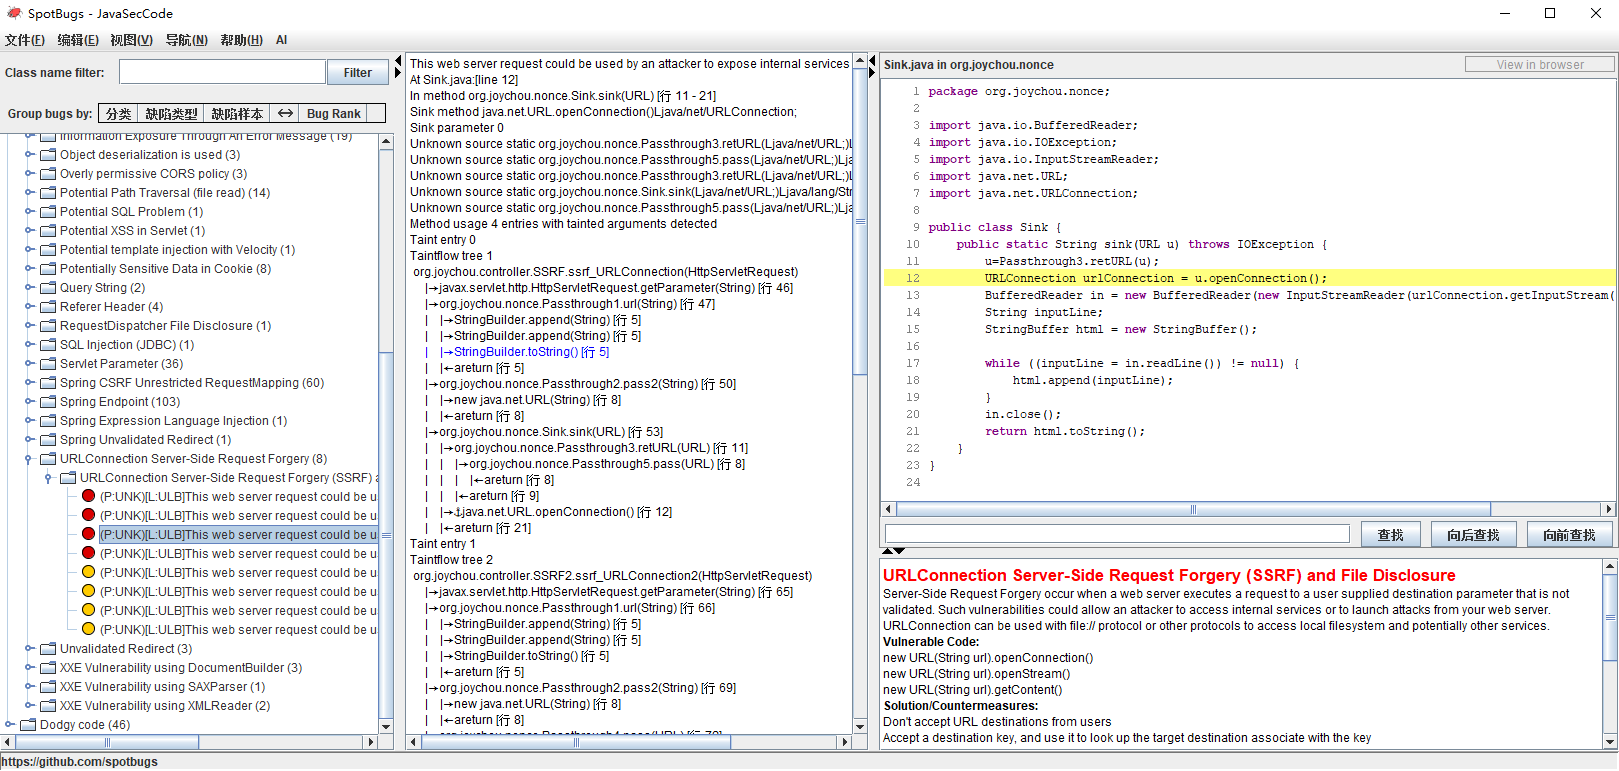
\includegraphics[width=0.8\linewidth]{FIGs/chapter4/taintAnalysis.png}
    \caption{污点分析结果界面}\label{show:taint}
\end{figure} 

图~\ref{show:settingServer} 展示了设置预测服务器的界面,点击上方菜单栏“AI”中的“Setting Remote Server”将会出现该界面,设置预测服务器是进行误报预测的首要步骤,在设置服务器窗口中,用户需要指定服务器的 URL 地址和管理员发放的 token。

% 设置预测服务器
 \begin{figure}[!htbp]
     \centering
     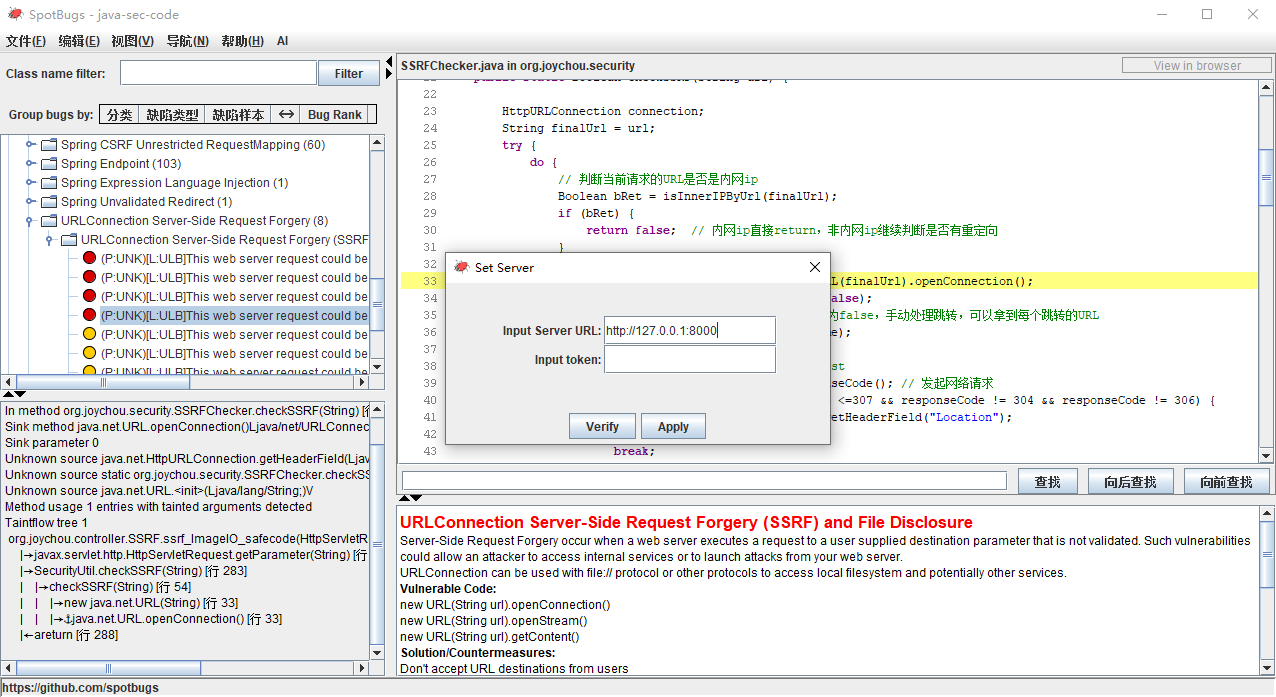
\includegraphics[width=0.8\linewidth]{FIGs/chapter4/settingServer.png}
     \caption{设置预测服务器界面}\label{show:settingServer}
 \end{figure} 

点击上方菜单栏“AI”中的“Slice and Predict”按钮,系统将对污点分析结果进行误报预测,图~\ref{show:predictResult} 展示了预测后一个被预测为误报的漏洞实例,在左上方,可以看到该漏洞实例的叶子节点已经变灰,且预测显示为“[P:FP]”(误报),在左下方,可以看到被预测为清洁函数的污染流已经由有清洁标记标注,这些标记用于向用户解释系统为何将其预测为误报。另外,可以看到图中的代码正是第二章中图~\ref{taintcase2} 中的代码,根据第二章的分析,该代码是为有效的 SSRF 修复代码,而本系统已经能够做出正确的预测,这证明了本系统确实可以根据先前的学习,排除误报。

% 预测结果
\begin{figure}[!htbp]
    \centering
    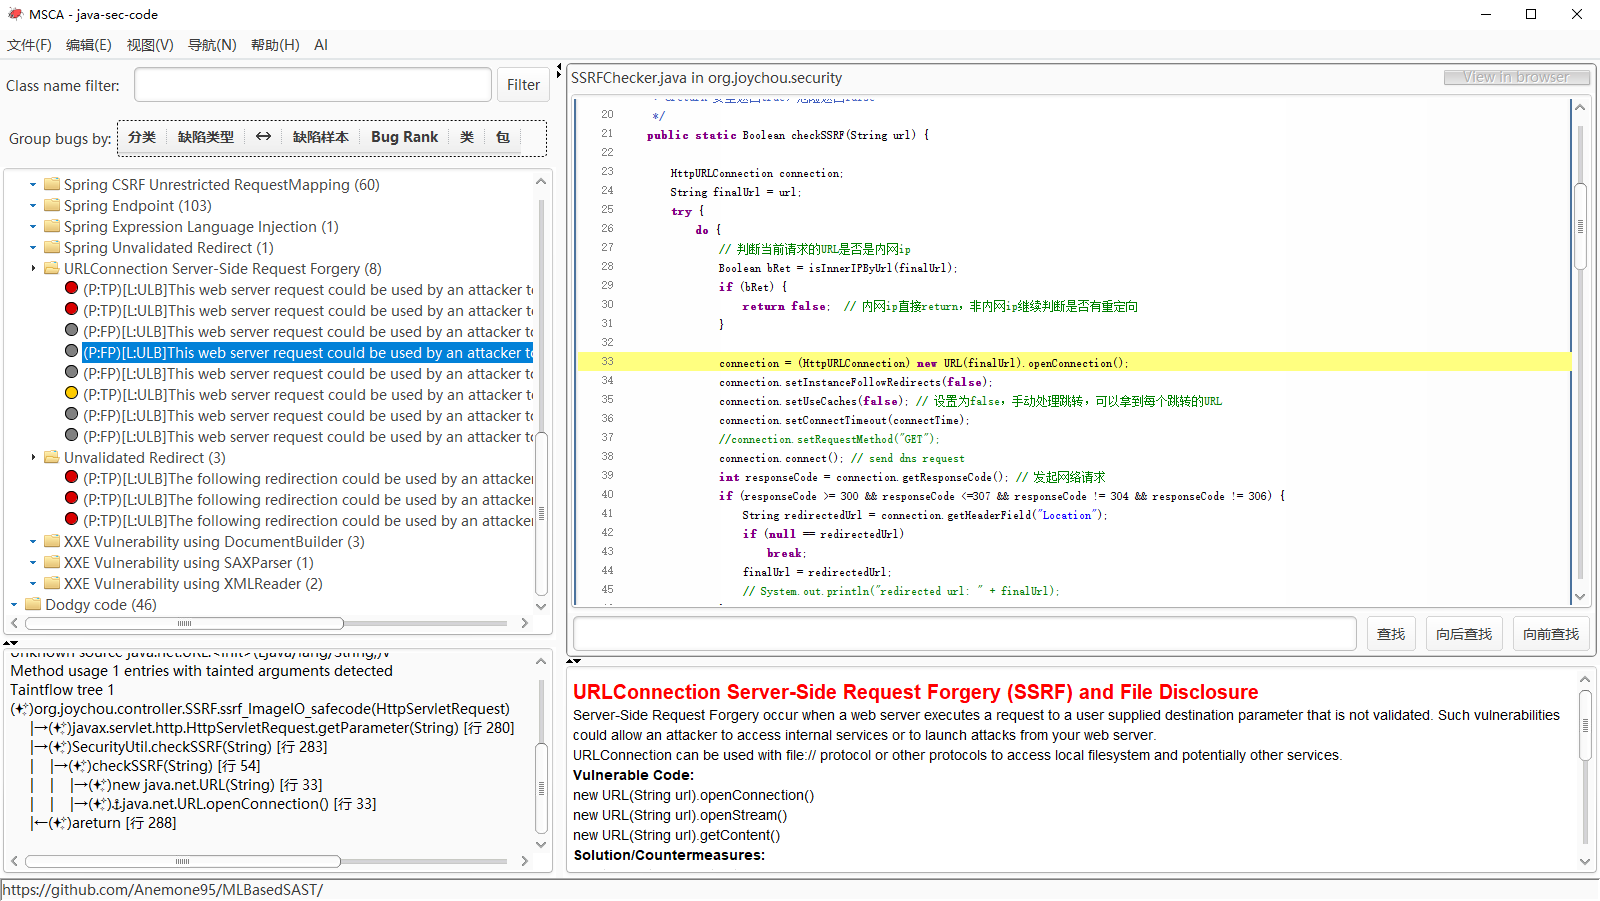
\includegraphics[width=0.8\linewidth]{FIGs/chapter4/predictResult.png}
    \caption{预测结果展示}\label{show:predictResult}
\end{figure}

对于报告中真实存在的漏洞,用户可以对其标记为正报,右击漏洞实例选择“Label as True Positive”即可弹出标记正报的界面,如图~\ref{show:labelTP} 所示,标记正报时用户必须在下拉菜单中选择一棵真实可以利用的污点传播树,点击提交后标记完成,完成后系统会更新左侧漏洞树,将“[L:ULB]”(未标记)转变为“[L:TP]”(标记为正报)。

% 标记正报
\begin{figure}[!htbp]
    \centering
    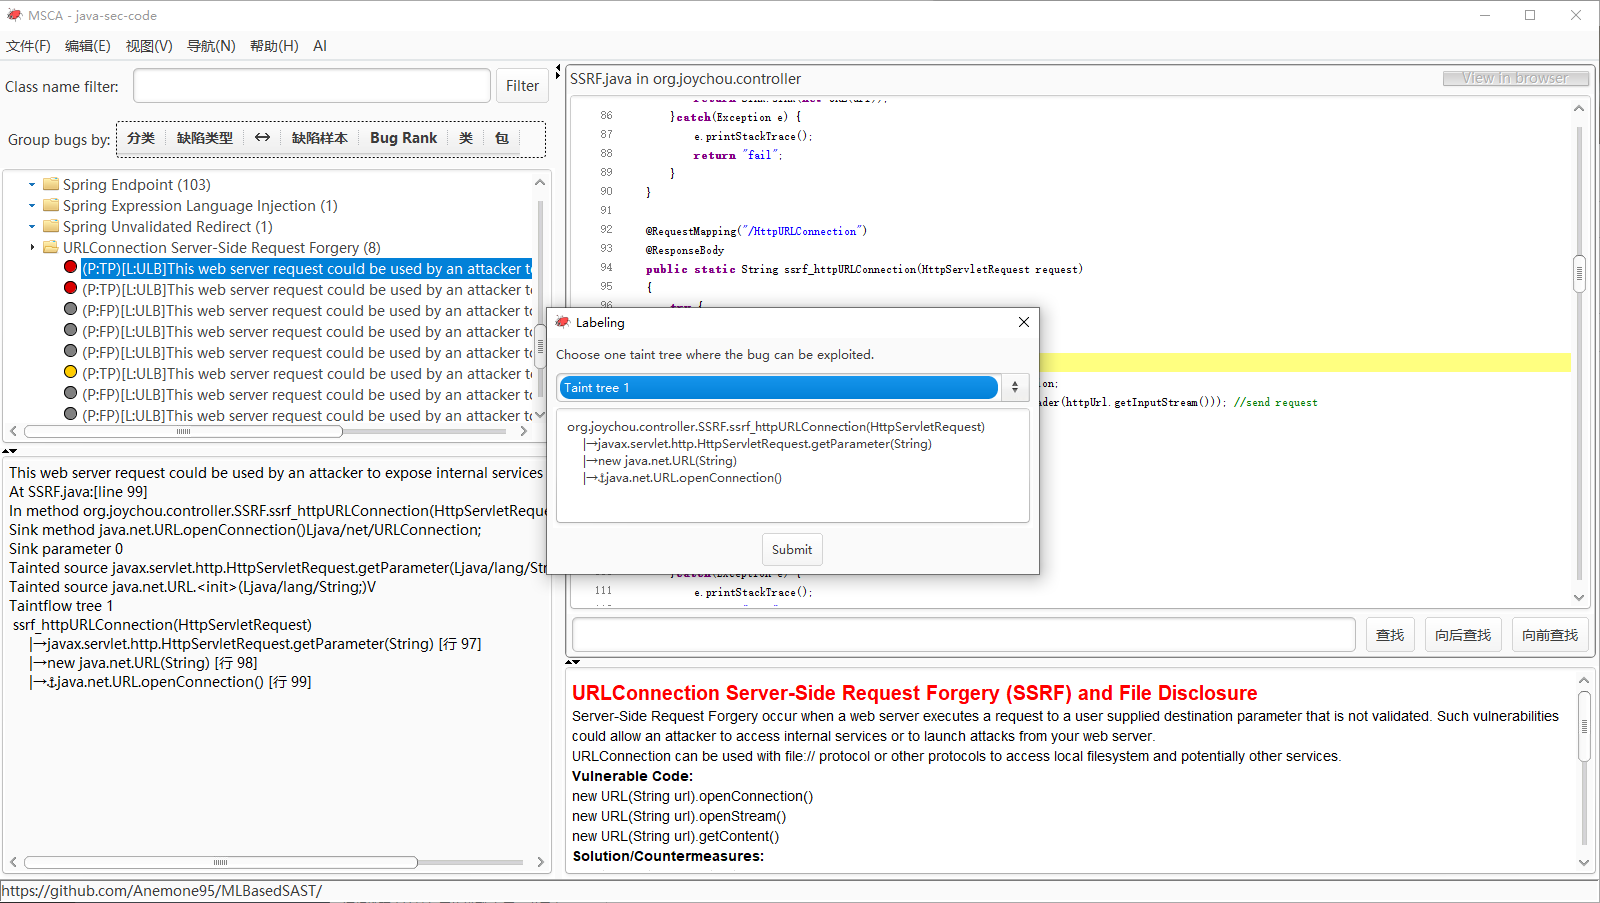
\includegraphics[width=0.8\linewidth]{FIGs/chapter4/labelTP.png}
    \caption{标记正报界面}\label{show:labelTP}
\end{figure}

对于报告中不可利用的正报漏洞,用户可以将其标记为误报,右击漏洞实例选择“Label as False Positive”即可弹出标记误报的界面,如图~\ref{show:labelFP} 所示,标记误报时用户需要在下拉菜单中指定一条污点传播流,同时用户可以在下方看到关于此污染流的切片内容,对误报的标记实际是对安全的污点传播流标记,标记完成后系统会重新计算并更新漏洞树,用户可以多次点击标记,直至该漏洞的标记变为“[L:FP]”(标记为误报)。

% 标记误报
\begin{figure}[!htbp]
    \centering
    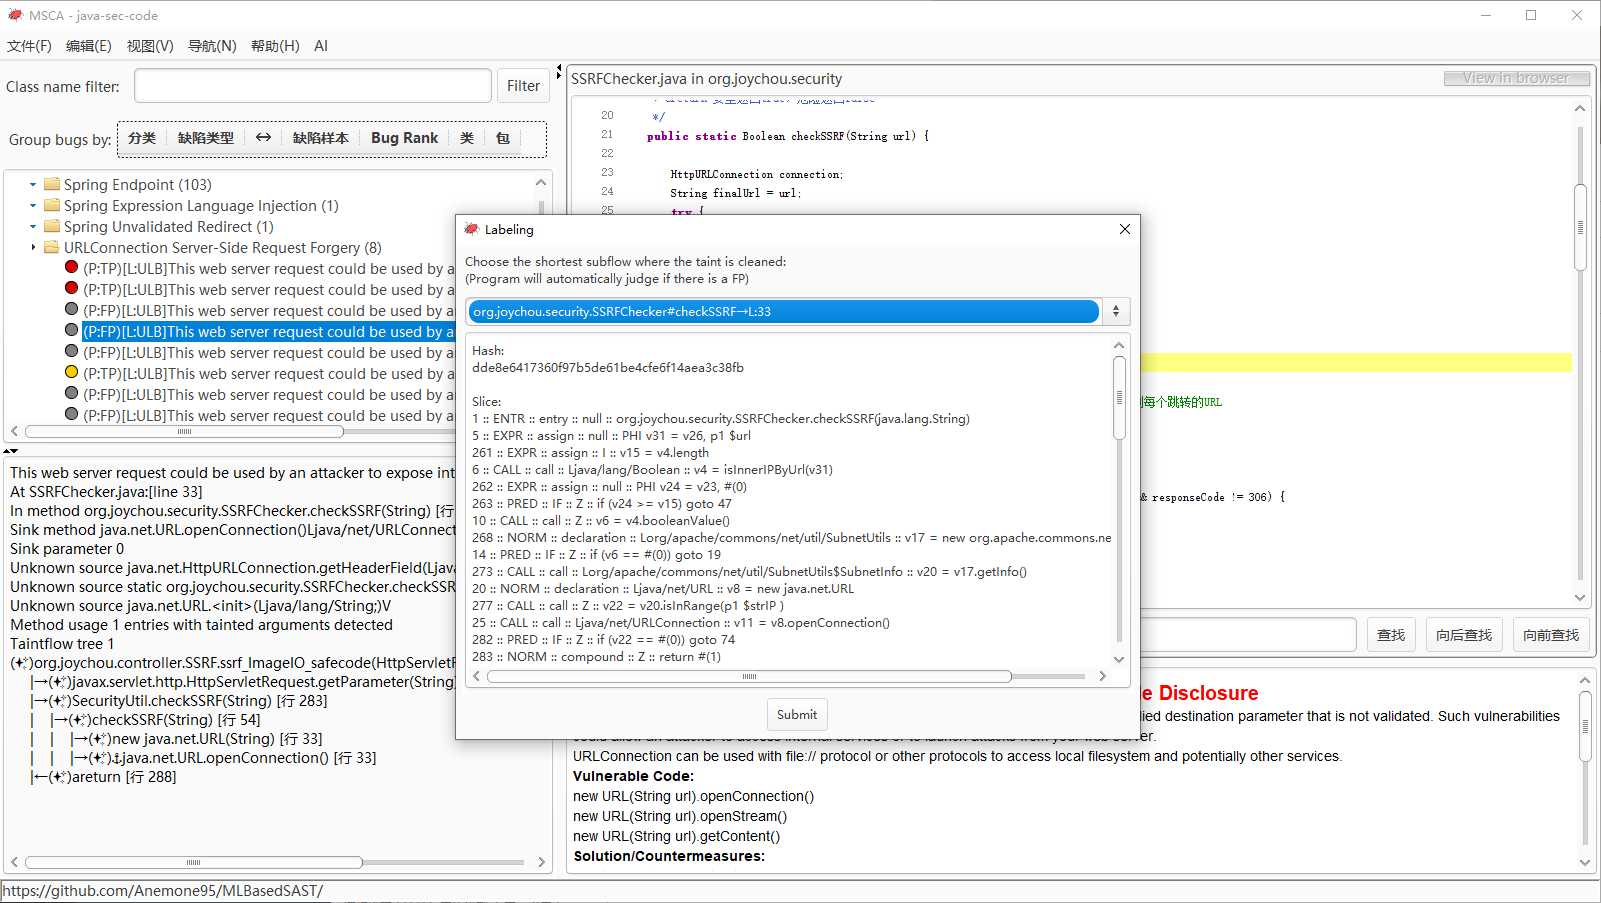
\includegraphics[width=0.8\linewidth]{FIGs/chapter4/labelFP.png}
    \caption{标记误报界面}\label{show:labelFP}
\end{figure}





\chapter{总结与展望}
\section{总结}
为了解决应用安全问题,本文设计了一套基于污点分析、程序切片和 BLSTM 的静态安全扫描系统,旨在从源头出遏制程序漏洞。相较于传统的污点分析类代码扫描系统,本系统对污点传播树进一步分析,通过程序切片和先前标记进行学习,能够有效地排除误报,保证扫描结果准确性,大大降低了系统使用时的人力成本。本文主要工作如下:


\begin{enumerate}
    \item 本文对开源污点传播工具 FindSecBugs 进行改造,使之能在报告中展示污点传播树,友好地向用户展示可能的漏洞利用过程。
    \item 系统对污点传播树进行拆分,将污点传播流和子传播流作为切片单位进行程序切片,系统优化了 Joana 切片过程,使之能够在缺失依赖、异构 Jar 包的情况下切片,并通过限制调用图限制程序切片范围,结合污点传播树的拆分,解决了目前切片资源消耗大导致扫描任务无法及时结束的问题。
    \item 系统根据实际情况对切片后的 SSA 进行泛化处理,进一步保证预测模型的泛化能力。
    \item 系统通过对漏洞的各个污点传播树的传播流及其子传播流进行预测,从而预测漏洞是否为误报。系统采用 BLSTM 模型,该模型在学术界已被多项工作证明其具在漏洞预测领域有较为显著的效果。用户在系统界面中能够得知漏洞预测结果,若为误报,系统能够清晰给出判断依据,即污点在哪一段传播流中无法继续传播,一定程度上弥补了深度学习可解释性差的问题。安全工程师能够轻松地对漏洞、传播树和传播流进行标记,并发起新的学习任务,不断提高预测模型的准确率。
\end{enumerate}

系统被设计为有良好的可拓展性,对于污点分析结果翻译、切片器和预测器,系统都对其高度抽象为接口,方便后期开发者在后期根据实际需要对系统中各个模块所用技术进行更换。

经过测试和实验,结果表明本系统具有较高的健壮性,在 Maven 仓库中前 100 流行度的项目中系统扫描成功率为 100 \%,此外,本系统具有较高准确性,在 OWASP 和 Juliet 的混合数据集中,本系统预测模块能够准确预测安全污点传播流,相较于 FindSecBugs,本系统在 OWASP 数据集上提高了约 20 \% 的准确率,减少了 25.44 \% 的误报。

\section{展望}

本系统是将深度学习在应用于漏洞扫描领域的一次成功探索,实现了传统检测技术与深度学习相结合,对于 Java 代码进行更准确的安全扫描任务,然而在未来,系统在以下方面还有较大的改进空间:

\begin{enumerate}
    \item 系统目前只针对 Java 语言,在未来可以将其方法推广到其他语言的项目中。
    \item 系统只能适用于能用污点分析方法分析的漏洞类型,在未来可以将切片和预测方法推广到其他基础分析的误报排除中。
    \item 系统并不能发现更多漏报,在未来可以使用类似的切片技术和预测方法,结合其他经典漏洞挖掘技术,在消除漏报方面做进一步提升。
    \item 系统在特征表示时,目前实际上是将切片转化为单词序列,再将单词序列进行向量化处理,在未来可以参考程序图特征表示的前沿工作,将切片表示成信息更丰富的特征,进一步提高预测准确性。
    \item 目前由于数据量有限,对于所有污点漏洞均使用一个模型进行预测,带数据量进一步扩大时,可以将针对每一种漏洞单独训练模型。
\end{enumerate}

% 参考文献

\bibliography{reference}
%% addde by lhy
%% 因为overleaf上没有这个参考文献排版文件
% \bibstyle{elsart-num}

\makeatletter
%preamble
\ifNJUT@review%
\else%

%个人简介
\Nchapter{简历与科研成果}
\noindent {\heiti 基本情况}
\vspace{1ex}
\noindent 徐文远,男,汉族,1995~年~8~月出生,江苏省南京市人。
\vspace{2ex}

\noindent {\heiti 教育背景}
\begin{description}[labelindent=0em, leftmargin=8em, style=sameline]
\item[2018.9~2020.6] 南京大学软件学院 \hfill 硕士
\item[2014.9~2018.6] 扬州大学信息工程学院 \hfill 本科
\end{description}
% 发表文章目录

\noindent {\heiti 科研项目}

\begin{enumerate}[label=\arabic*., labelindent=0em, leftmargin=*]
    \item 南京南瑞集团项目:调度自动化软件安全漏洞与风险实验能力提升关键技术研究,2018-2019。
\end{enumerate}

\noindent {\heiti 科研成果}

\begin{enumerate}[label=\arabic*., labelindent=0em, leftmargin=*]
    \item 房春荣、龚爱、\textbf{徐文远}、蒋燕、李玉莹、陈振宇,``一种基于Android源代码的风险等级预测方法'',申请号:201810092876.1,已受理。
\end{enumerate}

\backmatter


\begin{thanks}

\vskip 18pt

首先感谢陈振宇老师,感谢您两年以来对我的谆谆指导,不仅在学术上给我创造了很多机会,更重要的是教会我如何做人,让我如今能以一个研究生的身份走入社会。即使是在疫情严重时期,您也不断地牺牲个人时间通过线上会议和微信了解我们的毕设进展,提出宝贵意见,保证了本文的专业性和技术深度。感谢房春荣老师,在本项目的设计、实验安排等方面提出的宝贵建议和意见。同时感谢实验室黄勇老师在技术上的帮助和指导,是您的严格要求保证了本系统的健壮性。

感谢张双江、李灏宇师兄为本文的行文安排和格式上提供的帮助。感谢同为安全组的蒋燕和史洋洋同学,让我在科研的道路上不再孤单,感谢你们在平时研究和毕业设计过程中对我的帮助,在进展不顺利的时候给我安慰并与我一起出谋划策。

感谢 Koc 教授,是你们团队在学术上的工作为本文提供了理论支持,感谢 WALA 开发者 Manu,Joana 开发者 Simon,感谢你们的建议和意见让本文无依赖切片成为现实。

感谢暑期实习时与我一起工作的同事们,是你们让我了解到了真实安全运营时面临的问题,启发了本文的工作。

感谢父母,谢谢你们在我完成毕设期间对我的理解和支持,给我了一个舒适的工作环境,保证了毕设的顺利完成。


\end{thanks}

\fi%  
\makeatother

\end{document}


